% % Diplomarbeit Vorlage Tex V 000.1

%\documentclass[12pt,pdftex]{article}
\documentclass[12pt,pdftex,a4paper,titlepage]{scrreprt}
%\documentclass[12pt,pdftex,a4paper,titlepage]{article}
\usepackage[latin1]{inputenc}
\usepackage[T1]{fontenc}
\usepackage{ae}
\usepackage[ngerman]{babel}
\usepackage[ngerman]{varioref}
\usepackage{lmodern} %bessere Schriftart
\setlength{\parindent}{0pt} 
\usepackage{setspace} %
%\singlespacing%    Einfacher Zeilenabstand
%\onehalfspacing%    1 1/2 Zeilenabstand (entspricht angeblich den doppelten
% Zeilenabstand in Word)
\doublespacing%    Doppelter Zeilenabstand

\frenchspacing%     Kein doppeltes Leerzeichen nach '.' etc.

% Laden unterschiedlicher Pakete
%\usepackage{algorithmicx}
\usepackage{amsmath}
\usepackage{textcomp}
\usepackage{array}			 					% F�r formatierungen in Tabellen
\usepackage{color}	  		   		 			% Farben
\usepackage{framed}								% Einfache rechteckige Rahmenboxen
\usepackage{makeidx}							% Indexverzeichnis
\usepackage{wallpaper}
\usepackage{url}
\usepackage{pstricks, pst-node, pst-tree}  
\usepackage{floatflt}
\usepackage{listings,color}    					 %% color f�r Farbmarkierungen
\usepackage[a4paper,pdftex,top=2cm,left=3cm,right=2cm,bottom=2.5cm]{geometry}
%\usepackage[a4paper,pdftex,top=2cm,left=3cm,right=2cm,bottom=2.5cm,twoside]{geometry}
%\usepackage{pdfpages} komische fehlermeldung?!?
\usepackage[activate=normal]{pdfcprot}			% optischer Randausgleich
\usepackage{graphicx} 							% EPS grafiken
\usepackage{graphics}
\usepackage{epstopdf}							% eps grafiken in pdftex erlaubt
\usepackage{hyperref}
\usepackage{longtable}
\newcommand{\HRule}{\rule{\linewidth}{0.5mm}}
\usepackage{fancyhdr}
\pagestyle{fancy}
\addtolength{\headwidth}{\marginparsep}
\headheight=15pt
\fancyhf{}
\renewcommand{\sectionmark}[1]{\markright{\thesection\ #1}}
\rhead{\rightmark}
\renewcommand{\headrulewidth}{0.4pt}
% footer
\rfoot{\thepage}

%redefine plain pagestyle - used for chapter pages.
\fancypagestyle{plain}{
  \fancyhf{}
  \rfoot{\thepage}
  \renewcommand{\headrulewidth}{0pt}
}
\usepackage{multirow}

\usepackage{color}															 % f�r Farben im allgemeinen
\usepackage{colortbl}

\usepackage{hhline}
\usepackage{wrapfig}

% --- Farbdefinitionen ----------------------------------------
\definecolor{dunkelgrau}{rgb}{0.8,0.8,0.8}
\definecolor{hellgrau}{rgb}{0.95,0.95,0.95}


 \lstset{
   basicstyle=\small\ttfamily,
   keywordstyle=\bfseries\ttfamily\color{blue},
   stringstyle=\color{green}\ttfamily,
   commentstyle=\scriptsize\color{blue}\rmfamily,
   emph={square}, 
   emphstyle=\color{blue}\texttt,
   emph={[2]root,base},
   emphstyle={[2]\color{yac}\texttt},
   showstringspaces=false,
   flexiblecolumns=true,
   tabsize=2, 
   numbers=left,
   numberstyle=\small,
   numberblanklines=false,
   stepnumber=1,
   numbersep=10pt,
   xleftmargin=10pt,
   language=JAVA
 }
 
% Hyperref Einstellungen
\hypersetup{
 pdfauthor={Georg Wolf},
 pdftitle={Erstellung von Apps zum Einsatz auf Handys und Mobil-PCs zur
 Kommunikation mit Maschinen und Linien}, pdfsubject={Diplomarbeit, FH
 Gummersbach}, pdfkeywords={Diplomarbeit, Smartphone Apps, Android, iOS},
 backref=true,
 pagebackref=true,
 hyperfigures,
 hyperindex,
 colorlinks,
 bookmarksopen,
 bookmarksopenlevel=1,
 bookmarksnumbered,
 pageanchor,
 plainpages=false,
 % Hyperlink Farben:
 urlcolor=black,
 pagecolor=black,
 menucolor=black,
 citecolor=black,
 anchorcolor=black,
 filecolor=black,
 linkcolor=black,
 colorlinks=true, % Links einfaerben oder umranden
}

\setlength{\parindent}{0pt}	% Einr�cktiefe bei Abs�tzen einstellen
\setlength{\parskip}{1.5ex}	% Absatzabstand einstellen

% Mit folgenden Werten kann man die Silbentrennung einstellen (0..10000).
%\hyphenpenalty=10000 
%\exhyphenpenalty=10000
%\hyphenpenalty=10 \exhyphenpenalty=10

\setcounter{secnumdepth}{3}	% Hier stellt man ein bis zu welcher Ordnung �berschriften nummeriert werden (Beginnt bei 0 (Kapitel) und geht bis 5 (Subparagraph)
\setcounter{tocdepth}{3}	% Hier stellt man ein bis zu welcher Ordnung �berschriften ins Inhaltsverzeichnis �bernommen werden (ebenfalls 0 - 5)
%

\setlongtables

\graphicspath{{images/}{/global/images/}{anhang/}}	% Pfade f�r Grafiken angeben

\makeindex

% Anzahl und max. Seitenanteil von Abbildungen und Tabellen einstellen
\setcounter{topnumber}{5}
\setcounter{bottomnumber}{5}
\renewcommand{\bottomfraction}{.9}
\renewcommand{\textfloatsep}{3ex}
\renewcommand{\floatsep}{3ex}

% Nicht empfehlende Einstellungen:
%\sloppy    % Schlampige Absatzformatierung (wie M$ Word)
%\usepackage{wordlike}    % Simuliert M$ Word 



\setcounter{tocdepth}{1} 	%Gliederungstiefe im Inhaltsverzeichnis 
							%1 = nur erste und zweite ordnung

\begin{document}
%\maketitle

\onehalfspacing%    1 1/2 Zeilenabstand (entspricht angeblich den doppelten
% Zeilenabstand in Word)

%Leere Seite am Anfang
\newpage\thispagestyle{empty}~

% Titelblatt
\begin{titlepage}
\ifpdf\pdfbookmark{Titelseite}{title}\fi	% Zum PDF Inhaltsverzeichnis hinzuf�gen
\vspace*{1cm}
  
\includegraphics[scale=0.65]{fh_logo_schmal.eps} 
\thispagestyle{empty}
\begin{center}
  %\vspace{.5cm}
  %\huge{\sc bla}\\
  %\vspace{4cm}
  %\Large{\sc bla}\\
%  \vspace*{1cm}
%   	\textbf{Fachhochschule K�ln - Campus Gummersbach}\\
% 	Fakult�t f�r Informatik und Ingenieurwissenschaften\\
% \vspace*{1cm}
% 	\textbf{Cologne University of Applied Sciences}\\
% 	Faculty of Computer and Engineering Science\\
% \vspace*{1cm}
% 	Studiengang Allgemeine Informatik\\
% \vspace*{1cm}
%\HRule \\[0.4cm]
\vspace{3cm}
  	\Huge{\textbf{Diplomarbeit}\\}
  	\vspace*{3cm}
  	 \large{
  	zur Erlangung des Diplomgrades\\
	Diplom-Informatiker (FH)\\
	in der Fachrichtung Allgemeine Informatik\\}
  \vspace*{2cm}
  %\HRule \\[0.4cm]
%{ \huge  KHS }\\[0.4cm]
	\Large{\textbf{Erstellung von Smartphone Applikationen zur Kommunikation mit
	Fertigungsmaschinen}}\\ \vspace*{2.0cm}
%\HRule \\[1.5cm]

 \begin{tabular}{ll} 
 \large Von: 			& \large Georg Wolf \\
 						& \large Matr-Nr.: 11052530\\
 \large Erstpr�fer: 	& \large Prof. Friedbert Jochum\\
 \large Zweitpr�fer: 	& \large ? (Poborski/Klocke)\\
 \large vorgelegt: 		&\ \today\\
 \end{tabular}
  
  %\vspace*{1cm}
  
  %\vspace{2cm} 
  \end{center} 
\end{titlepage}

%\renewcommand{\abstractname}{Abstract}
%\abstract 
\begin{minipage}[b]{1\linewidth}
\chapter*{\abstractname}\label{zusammenfassung}
\ifpdf\pdfbookmark{\abstractname}{abstract}\fi	% Zum PDF Inhaltsverzeichnis hinzuf�gen
Hier folgt eine kurze Zusammenfassung des Themas (ca. 5~
Zeilen).
\end{minipage}

\begin{minipage}[b]{1\linewidth}
\chapter*{Abstract}
Short description of the thesis (probably 5 lines).
\end{minipage}

\chapter*{Vorwort}\label{vorwort}
\ifpdf\pdfbookmark{Vorwort}{vorwort}\fi % Zum PDF Inhaltsverzeichnis hinzuf�gen

Motivation (warum habe ich mich f�r dieses Thema
entschieden)\ldots

\begin{itemize}
  \item Im Studium WPF Handyprogrammierung mit JavaME
  \item Interesse an Smartphoneprogrammierung
  \item Apps als boomendes Marketinginstrument erkannt
\end{itemize}

\begin{minipage}[b]{1\linewidth}
\chapter*{Danksagung}

%Ich bedanke mich f�r die Unterst�tzung bei\ldots! Ferner m�chte
%ich\ldots danken.

Zuerst m�chte ich mich bei meinen Eltern bedanken, die mich mein ganzes Studium
�ber unterst�tzt haben. Ohne Sie h�tte ich es nicht geschafft �berhaupt noch
einmal zu studieren.\\

%todo: check, ob man den langen titel wirklich so ausschreibt oder irgendwie
% abk�rzt
Ferner danke ich meinem Mentor Herrn Prof. Friedbert Jochum, der mich �ber den
Zeitraum meiner Diplomarbeit betreute und mir immer wieder neue Anregungen und
Aspekte aufzeigte, um meine Abschlussarbeit in die richtige Richtung zu
lenken.\\

Nicht zu vergessen nat�rlich die Firma KHS GmbH, die mir die
M�glichkeit gegeben hat meine Diplomarbeit in Ihrem Hause zu schreiben.
Besonders zu erw�hnen sind hier Herr F�rster, mein direkter Ansprechpartner,
sowie Herr Buchkremer und Frau Kholodenko, die immer ein offenes Ohr f�r mich
hatten. (Fari?)\\

Dank gilt auch meinen geduldigen Korrekturlesern Oliver Pol und Maik
``Sch�pperts'' E. Vielen Danke f�r die investierte M�he, Zeit und Rotstifte.

\end{minipage}

\ifpdf\pdfbookmark{\contentsname}{tableofcontents}\fi%   PDF Bookmark Eintrag fuer das Inhaltsverzeichnis.
{\singlespacing
\tableofcontents
}
%\doublespacing
\onehalfspacing

\newpage
\listoffigures   % Abbildungsverzeichnis
\newpage
\listoftables    % Tabellenverzeichnis
%Abk�rzungsverzeichnis
\newpage
\chapter*{Abk�rzungsverzeichnis}
%\ifpdf\pdfbookmark{\abkuerzungsverzeichnis}{abkuerzungsverzeichnis}\fi

HMI - Human Machine Interaction\\
Visu-Station - Visualisierungs-Station\\
Apps - ist die Abk�rzung von ''Applications''. Gemeint sind zus�tzliche
Anwendungen f�r Smartphones\\
SDK - Software Developers/Development Kit\\
DVM - Dalvik Virtual Machine\\
MVC - Model-View-Controller\\
SSH - \\
Jailbreak - \\
IDE - \\
ADT - \\
MDA - \\
IRDA - \\
XOR - \\
Brute-Force - \\ %ins abk�rzungsverzeichnis? muss aber trotzdem erkl�rt werden
MAC-Adresse - \\
OMG - Object Management Group\\
EAP-TLS - \\
EAP-TTLS - \\
PEAP - \\
LEAP - \\
SIMs - \\
RFC - \\
WEP - \\
WLAN - \\
WPA - Wi-Fi Protected Access \\
TKIP - Temporal Key Integrity Protocol\\
AES - Advanced Encryption Standard\\
MAC - \\
GSM - \\
BTS - \\
GPRS - \\
CI - Corporate Identity \\
GAF - Gesch�ftsvorfall\\
ITU - \\
XMI - XML Meta-Data Interchange\\
DSL - Domain Specific Language\\
MOF - Meta Object Facility\\









\chapter{Einleitung und Aufgabenstellung}
\begin{itemize}
  \item Kontext f�r den/die Leser herstellen
  \item Am besten schreiben, wenn die Arbeit im groben fertig ist
\end{itemize}
	%\section{Motivation}
		
	\section{Zielsetzung und Beschreibung der Aufgabenstellung}
    
    Ziel dieser Arbeit ist es aufzuzeigen, ob die Kommunikation zwischen einer
    Fertigungsmaschine und einem Smartphone sinnvoll ist, und welche konkreten
    Vorteile dies bietet im Vergleich zu einer Feststation mit HMI.
      
    Als L�sungsanbieter f�r Abf�ll- und Verpackungsanlagen stellt KHS
    Fertigungsmaschinen f�r die Industrie her. Die Bedienung dieser Maschinen
    beim Kunden erfolgte in der Vergangenheit direkt an der Maschine �ber das
    Human Machine Interface (sp�ter als HMI bezeichnet).
    
    Auf Grund der steigenden Verbreitung von Smartphones und der damit
    verbundenen M�glichkeiten soll nun im Rahmen dieser Diplomarbeit �berpr�ft
    werden, inwiefern eine Kommunikation zwischen einer Smartphone Applikation
    und einer von KHS hergestellten Fertigungsmaschine sinnvoll sein kann. Es
    werden hier nicht nur die technischen Rahmenbedingungen gekl�rt, sondern
    auch wirtschaftliche Aspekte im Hinblick auf Verbreitung und Marketing
    aufgezeigt.
    
    Dabei sollen verschiedene Modelle von derzeit gebr�uchlichen Smartphones
    untersucht werden im Hinblich auf Einstiegsbeschr�nkungen zur Entwicklung
    und die Komplexit�t eine solche Anwendung zu erstellen. Auch
    Zusatzkosten spielen hier eine Rolle. Es sollen
    m�glichst viele Smartphones bedient werden k�nnen. Dies bedeutet in der
    Entwicklung einen erheblichen Aufwand, da sich die einzelnen mobilen
    Endger�te sehr unterscheiden. �ber den Ansatz der ``Model Driven
    Architecture'' wird ein generisches Konzept f�r eine
    Applikation entwickelt und erl�utert wie sich dieses im Anschluss f�r
    verschiedene Endger�te umsetzen l�sst. M�gliche L�sungsans�tze f�r diese
    Probleme werden konkret aufgezeigt.
    
    Weiterhin relevant stellen sich die Rahmenbedingungen der
    Smartphonehersteller dar. In dieser Arbeit wird dargelegt, welche
    speziellen Restriktionen sich nicht nur allgemein in der Hardware befinden
    (Display, Prozessor, spezielle Funktionen der Ger�te), sondern speziell
    auch vom Hersteller vorgegeben werden. Unter anderem die Voraussetzungen
    f�r die entsprechende Hardware entwickeln zu k�nnen. Bei den meisten
    Open-Source Betriebssystemen steht die Wahl der Entwicklungshardware und
    -umgebung relativ frei. 
    
%     Ein gutes Beispiel ist hier Android, welches dem
%     Entwickler v�llig freie Hand l�sst. Bei der der Entwicklung entstehen
%     nur die tats�chlichen Kosten f�r die Programmierung, da die Entwicklungsumgebung
%     (SDK) kostenfrei von Google zur Verf�gung gestellt wird. Ganz im Gegenteil
%     zum Mitbewerber Apple, bei dem auch die Entwicklungshardware vom selbigen
%     Hersteller eingekauft werden muss. Zwar ist es m�glich, seine Applikationen
%     in Apples eigens daf�r vorgesehenem Simulator zu testen. F�r einen
%     Test auf dem eigentlichen Ger�t jedoch muss der Umweg �ber den Apple App
%     Store gegangen werden. [Koller10]
    
    Ein konkretes Programm soll in Form eines Prototyps erst genau spezifiziert,
    dann mit Hilfe der Modellgetriebenen Softwareentwicklung (kurz MDA)
    ansatzweise auf m�glichst viele mobile Endger�te umsetzbar gemacht werden.  
    
    Es werden verschiedene Erwartungshaltungen formuliert im Hinblick auf die
    unterschiedlichen Eigenschaften der Endger�te. Bei der Softwareerstellung
    muss vermehrt auf diese Restriktionen eingegangen werden. Ein kleines Display
    und diverse andere Eigenschaften der Smartphones m�ssen durch ein
    geeignetes Design des Userinterfaces abgedeckt werden.
   
    Diese Diplomarbeit soll als Grundger�st f�r zuk�nftige Entscheidungen und
    Entwicklungen im Bereich Apps f�r Smartphones dienen und einen konkreten
    Anhaltspunkt dar�ber geben, ob Entwicklung in dieser Sparte �berhaupt
    sinnvoll erscheint.
    
    \section{Das Unternehmen KHS}
		%\begin{itemize}
        	%\item kurz eingehen auf Geschichte KHS (1-2 abs�tze)
        	%\item Standorte und aufgabengebiete/tagesgesch�ft
        %\end{itemize}
        
        %TODO: mehr????
        Diese Diplomarbeit wird als Studie f�r die KHS GmbH erstellt. 
        
        \begin{quote}      
        ``KHS ist L�sungsanbieter technologisch innovativer und
        hochwertiger Abf�ll- und Verpackungsanlagen f�r die Getr�nke- und
        Nahrungsmittelindustrie. Mit mehr als 5.500 Mitarbeitern weltweit
        realisiert der zentral von Dortmund aus gef�hrte Konzern heute einen
        Jahresumsatz von fast einer Milliarde Euro. Neben Produktionsst�tten
        in den USA, Mexiko, Brasilien, Indien und China ist KHS mit mehreren
        Werken in Deutschland vertreten.

		Das Unternehmen ist eine 100-prozentige Tochtergesellschaft der Salzgitter
		AG, einem der f�hrenden Stahl- und Technologie-Konzerne Europas.

		Seit 2008 sind die Unternehmen KHS Corpoplast, KHS Plasmax, KHS Moldtec und
		KHS Asbofill in den Kl�ckner-Konzern integriert. Damit ist die KHS
		insbesondere im Bereich ganzheitlicher PET-L�sungen bestens aufgestellt. Durch
		neue Entwicklungen wie Trockenteil-L�sungen in Modulbauweise, universelle
		F�llsysteme, Hochleistungs-Etikettiertechnik oder moderne Kommunikations- und
		Diagnosetechniken festigt die KHS fortlaufend ihre Position als Innovator im
		Markt.'' [KHS10], letzter Abruf: 21.11.2010
		\end{quote} 
        
		
        
    
% 		\begin{itemize}
%           \item Entwicklung von KHS Apps f�r Handys zur Kommunikation mit
%           Maschinen und Linien der KHS
%         \end{itemize}
        
%         Dazu werden verschiedene Aspekte eruiert hinsichtlich 

% \chapter{Kapitelname}
% 
% \section{�berschrift 1. Ordnung}
% 
% \subsection{�berschrift 2. Ordnung}
% 
% \subsubsection{�berschrift 3. Ordnung}
% 
% \paragraph{�berschrift 4. Ordnung}
% 
% \subparagraph{�berschrift 5. Ordnung}
% 
% \begin{center}
% Zentrierter Text
% \end{center}
% 
% \begin{flushleft}
% Linksseitiger Text
% \end{flushleft}
% 
% \begin{flushright}
% Rechtsseitiger Text
% \end{flushright}
% 
% Verschiedene Schriftformen:
% \\ % ein Zeilenumbruch
% \textit{Kursiver Text}
% \textsl{Schr�g gestellter Text} % Unterschied zu kursiv = ???
% \textbf{Fettgedruckter Text} 
% \textsc{Text in Kapit�lchen} 
% \texttt{Text in Nicht-Proportionalschrift}
% \par % Neuer Absatz (explizite Form)
% \newpage % Neue Seite erzwingen
% 
% Eine Auflistung:
% \begin{itemize}
% \item Eins
% \item Zwei
% \item Drei
% \end{itemize} 
% 
% \bigskip % einen gr��eren Abstand einf�gen
% 
% Eine durchnummerierte Aufz�hlung:
% \begin{enumerate}
% \item Eins
% \item Zwei
% \item Drei
% \end{enumerate} 
% 
% \bigskip % einen gr��eren Abstand einf�gen
% 
% Eine Beschreibungsumgebung:
% \begin{description}
% \item[Zu beschreibender Begriff] Beschreibender Text
% \item[Noch ein zu beschreibender Begriff] Ein langer Text der den Begriff beschreibt wird automatisch einger�ckt wenn er l�nger als eine Zeile ist. Das sieht dann so aus. 
% \end{description} 
% 
% %\begin{list}{Label}{}
% %\item Eins
% %\item Zwei
% %\end{list} 
% 
% \newpage
% \section{Tabellen}
% 
% Es gibt Tabellen die fest im Text verankert sind. Sie erscheinen immer dort und k�nnen keine Tabellebezeichnung und somit keine Nummer bekommen:\\
% 
% \begin{tabular}{ccc}	% eigentliche Tabellenumgebung beginnen: {ccc} = 3 Spalten, zentriert
% \hline			% horizontale Linie
%  Ich bin & ein feste & Tabelle \\ % Spalten mit & trennen und Zeile mit \\ beenden
% \hline\hline		% doppelte horizontale Linie
%  a & b & c \\ 		% n�chste Zeile
% \hline			% horizontale Linie
% \end{tabular} 
% 
% Besser sind aber die gleitenden Tabellen. Man kann angeben wo sie erscheinen sollen: An der Stelle wo man sie hingeschrieben hat, oben an der Seite, unten an der Seite oder auf einer extra Seite nru f�r gleitende Objekte. 
% 
% % Beispiel f�r eine gleitende Tabelle
% \begin{table}	% Gleitende Tabelle beginnen: Position am besten bei: h = here, t = top, b = bottom, p = page (auf eigener Seite) - LaTex versucht die Positionierung in dieser Reihenfolge
% % Die Angabe nur von "h" um die Positionierung an einer Stelle zu erzwingen l��t LaTeX nicht zu, wenn die Tabelle dann an einer unm�glichen Stelle erscheinen w�rde
% \centering \leavevmode	% zentrieren
% \caption{Eine gleitende Tabelle}	% Tabellenbeschrieftung
% \begin{tabular}{ccc}	% eigentliche Tabellenumgebung beginnen: {ccc} = 3 Spalten zentriert
% \hline			% horizontale Linie
%  Name & Vorname & Sonstiges \\ % Spalten mit & trennen und Zeile mit \\ beenden
% \hline\hline		% doppelte horizontale Linie
%   & b & c \\ 		% n�chste Zeile
% \cline{2-3}		% horizontale Linie, nur von Spalte 2 bis 3
%  \raisebox{1.5ex}[-1.5ex]{A} & b & c \\ 	% Text �ber zwei Zeilen: Zeile vorher freilassen, diese Zeile mit \raisebox{h�he}[-h�he]{Text} hochheben (1ex = normale Zeilenh�he)
% \multicolumn{2}{c}{Doppelspaltig} & c \\
% \hline			% horizontale Linie
% \end{tabular} 
% \end{table}
% 
% % Noch ein Beispiel f�r eine gleitende Tabelle
% \begin{table}	% Gleitende Tabelle beginnen
% \centering \leavevmode	% zentrieren
% \caption{Eine andere gleitende Tabelle}	% Tabellenbeschrieftung
% % eigentliche Tabellenumgebung beginnen:
% \begin{tabular}{|l|c|p{0.5cm}|r|}	 % | = vert. Strich, l = links, c = zentriert, p{breite} = feste Breite, r = rechts
% % Also: hier vier Spalten mit vertikalen Linien. Sie sind links, mittig, 0.5cm breit und rechts ausgerichtet.
% \hline			% horizontale Linie
%  Name & Vorname & \# & Sonstiges \\ % Spalten mit & trennen und Zeile mit \\ beenden
% \hline\hline		% doppelte horizontale Linie
%  a & b & 0 & c \\ 		% n�chste Zeile
% \hline			% horizontale Linie
% \end{tabular} 
% \end{table}
% 
% Um eine �berlange Tabelle �ber mehrere Seiten zu erzeugen statt die tabular die longtable Umgebung (Paket longtable) verwenden. Ein Beispiel findet man im Fu�notenabschnitt.
% 
% \newpage	% neue Seite einleiten (Achtung: ggf. schlechter Stil!)
% \section{Bilder}
% 
% \begin{figure}	% Beginn des gleitenden Bildes
%    \centering	% zentrieren
%    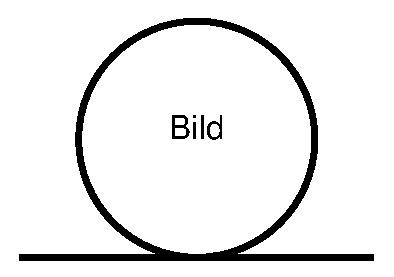
\includegraphics[scale=0.5]{beispiel}% Bild einf�gen. Am besten nur Dateinamen ohne Erweiterung angeben; hier um Faktor 0.5 skaliert
%    \caption{Ein Beispielbild (skaliert)}	% Bildbezeichnung
%    \label{fig:beispiel1}	% Interne Bezeichnung um Bild im Text referenzieren zu k�nnen
% \end{figure}
% 
% \begin{figure}	% Beginn des gleitenden Bildes
%    \centering	% zentrieren
%    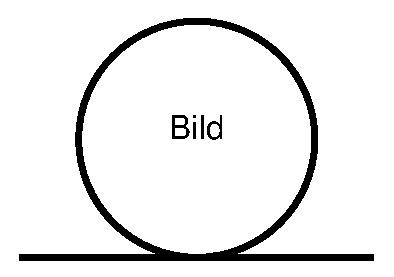
\includegraphics[scale=0.5,angle=45]{beispiel}% Bild einf�gen. Um Faktor 0.5 skaliert und um 45 Grad gegen den Uhrzeigersinn gedreht
%    \caption{Ein gedrehtes Beispielbild}	% Bildbezeichnung
%    \label{fig:beispiel2}	% Interne Bezeichnung um Bild im Text referenzieren zu k�nnen
% \end{figure}
% 
% \begin{figure}	% Beginn des gleitenden Bildes
%    \centering	% zentrieren
%    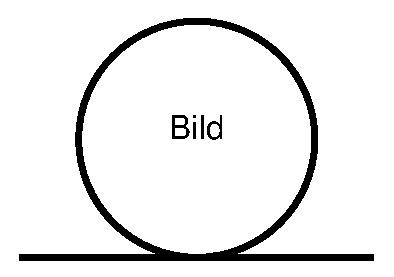
\includegraphics[width=0.6\textwidth]{beispiel}% Bild einf�gen. Auf 60% der Textbreite skalieren
%    \caption{Ein Beispielbild mit 60\% der Textbreite}	% Bildbezeichnung
%    \label{fig:beispiel3}	% Interne Bezeichnung um Bild im Text referenzieren zu k�nnen
% \end{figure}
% 
% \begin{figure}	% Beginn des gleitenden Bildes
%    \centering	% zentrieren
%    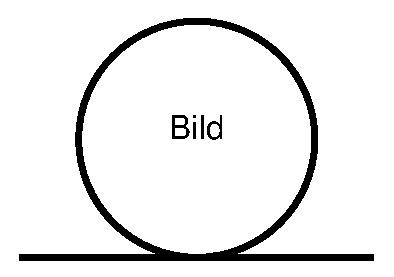
\includegraphics[height=1cm,width=2cm]{beispiel}% Bild einf�gen. H�he auf 1cm und Breite auf 2cm festlegen
%    \caption{Ein Beispielbild, 1cm hoch und 2cm breit}	% Bildbezeichnung
%    \label{fig:beispiel4}	% Interne Bezeichnung um Bild im Text referenzieren zu k�nnen
% \end{figure}
% 
% \begin{figure}	% Beginn des gleitenden Bildes
%    \centering	% zentrieren
%    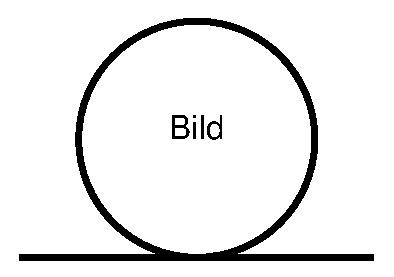
\includegraphics[draft]{beispiel} % Bild einf�gen aber nicht anzeigen, sondern anstatt einen Rahmen mit dem Pfad einblenden (kann auch global mit \usepackage[draft]{graphicx} im Pr�ambel eingestellt werden)
%    \caption{Ein Beispielbild, nur Platzhalter mit Bildpfad dargestellt}	% Bildbezeichnung
%    \label{fig:beispiel5}	% Interne Bezeichnung um Bild im Text referenzieren zu k�nnen
% \end{figure}
% 
% Und so referenziert man ein Bild: Bild \ref{fig:beispiel2} auf Seite \pageref{fig:beispiel2} zeigt ein Beispiel. Geht auch vor dem referenzierten Bild wie man bei Bild \ref{fig:beispiel6} auf \pageref{fig:beispiel6} sieht.
% 
% \begin{figure}	% Beginn des gleitenden Bildes
%    \centering	% zentrieren
%    \framebox{	% Erzeugt Rahmen um das Bild
%    	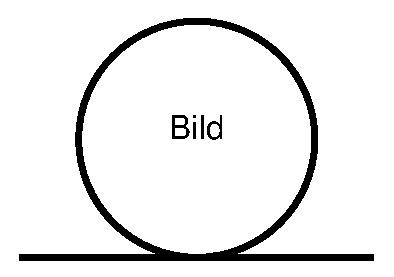
\includegraphics[bb=20 50 110 100,clip]{beispiel} % Bild mit der angegebenen BoundingBox (bb=x1 y1 x2 y2) clippen
%    } % Ende von \framebox{
%    \caption{Ein Ausschnitt des Beispielbildes mit Rahmung}	% Bildbezeichnung
%    \label{fig:beispiel6}	% Interne Bezeichnung um Bild im Text referenzieren zu k�nnen
% \end{figure}
% 
% \clearpage	% neue Seite einleiten, alle Gleitobjekte (Tabellen, Bilder) anzeigen
% \subsection{Zwei Bilder nebeneinander}
% 
% \begin{figure}
%    \centering	% zentrieren
%    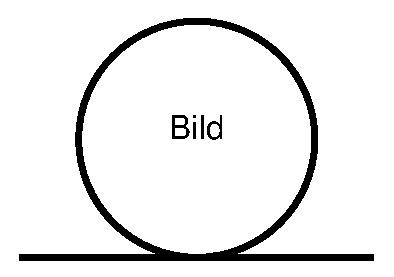
\includegraphics[scale=0.5]{beispiel}	% erstes Bild
%    \quad					% Ein wenig Abstand dazwischen (/qquad w�re ein gr��erer Abstand)
%    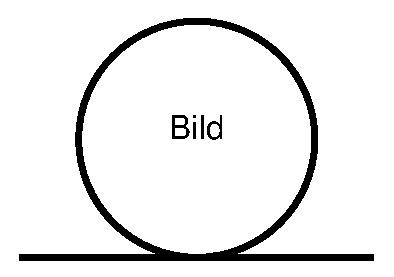
\includegraphics[scale=0.5]{beispiel}	% zweites Bild
%    \caption{Zwei Bilder mit einer gemeinsamen Bildunterschrift}	% Bildbezeichnung
%    \label{fig:beispiel7}	% Interne Bezeichnung um Bild im Text referenzieren zu k�nnen
% \end{figure}
% Sind die Bilder zu gro� um nebeneinader dargestellt zu werden, werden sie untereinander dargestellt:
% 
% \begin{figure}
%    \centering	% zentrieren
%    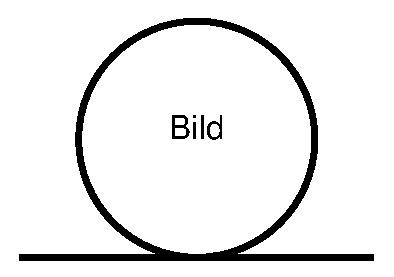
\includegraphics[width=0.6\textwidth]{beispiel}	% erstes Bild (k�nstlich vergr��ert)
%    \quad					% Ein wenig Abstand dazwischen (hier sinnvoll?)
%    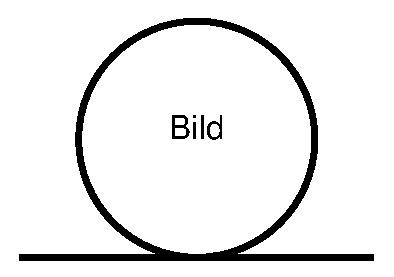
\includegraphics[width=0.6\textwidth]{beispiel}	% zweites Bild (k�nstlich vergr��ert)
%    \caption{Zwei gro�e Bilder mit einer gemeinsamen Bildunterschrift}	% Bildbezeichnung
%    \label{fig:beispiel8}	% Interne Bezeichnung um Bild im Text referenzieren zu k�nnen
% \end{figure}
% 
% Um das zu verhindern kann man eine makebox (oder eine framebox) um die Bilder ziehen. Dann wird aber u.U. in den Rand gezeichnet. Beispiel:
% 
% \begin{figure}
%    \centering	% zentrieren
%    \framebox[\textwidth]{	% framebox (=Rahmen) mit der Breite des Textes erzeugen
%    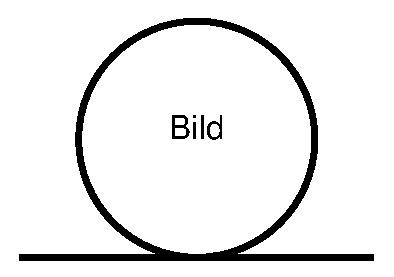
\includegraphics[width=0.6\textwidth]{beispiel}	% erstes Bild (k�nstlich vergr��ert)
%    \quad					% Ein wenig Abstand dazwischen
%    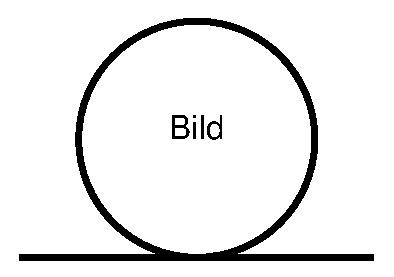
\includegraphics[width=0.6\textwidth]{beispiel}	% zweites Bild (k�nstlich vergr��ert)
%    }
%    \caption{Zwei gro�e Bilder in einer Framebox}	% Bildbezeichnung
%    \label{fig:beispiel9}	% Interne Bezeichnung um Bild im Text referenzieren zu k�nnen
% \end{figure}
% 
% \clearpage
% Hier nun zwei Bilder nebeneinander mit jeweils eigener Bildbeschreibung:
% 
% \begin{figure}
%   \begin{minipage}[t]{0.48\textwidth}	% Minipage erzeugen, [t] = Am oberen Rand ausrichten
%       \centering	% zentrieren
%       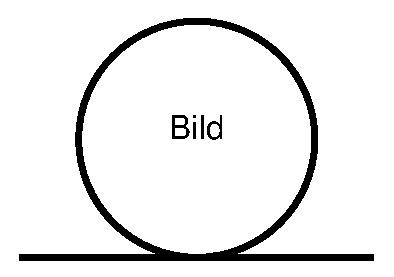
\includegraphics[width=0.48\textwidth]{beispiel}
%       \caption{Linkes Beispielbild (mit einem l�ngeren Text als das rechte Bild)}
%       \label{fig:beispiel10}
%   \end{minipage}% Dies Prozent ist wichtig! (kein horiz. Abst. zw. minipages)
%   \begin{minipage}{0.04\textwidth}
%      \hfill % Damit die getrennte Beschriftung auch Abstand hat
%   \end{minipage}%
%   \begin{minipage}[t]{0.48\textwidth}
%       \centering	% zentrieren
%       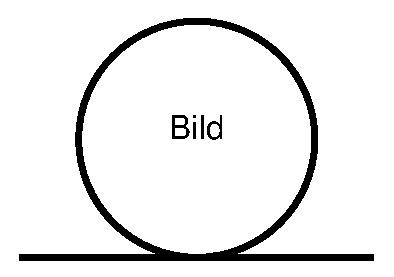
\includegraphics[width=0.48\textwidth]{beispiel}
%       \caption{Rechtes Beispielbild}
%       \label{fig:beispiel11}
%   \end{minipage}
% \end{figure}
% 
% Da die Bilder gleich gro� sind richten wir sie nach oben aus damit sie aufgrund der unterschiedlich langen Beschreibungstexte nicht horizontal verschoben werden. \\
% Anonsten sollte man sie wohl unten ausrichten: (oder zentrieren)
% 
% \begin{figure}
%   \begin{minipage}[b]{0.48\textwidth}
%       \centering	% zentrieren
%       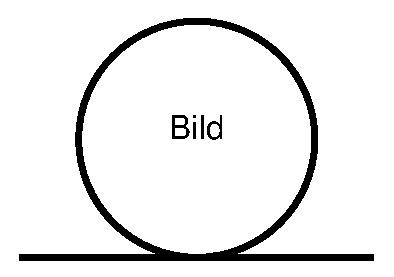
\includegraphics[width=0.48\textwidth]{beispiel}
%       \caption{Linkes Beispielbild (mit einem l�ngeren Text als das rechte Bild)}
%       \label{fig:beispiel12}
%   \end{minipage}% Dies Prozent ist wichtig! (kein horiz. Abst. zw. minipages)
%   \begin{minipage}{0.04\textwidth}
%      \hfill % Damit die getrennte Beschriftung auch Abstand hat
%   \end{minipage}%
%   \begin{minipage}[b]{0.48\textwidth}
%       \centering	% zentrieren
%       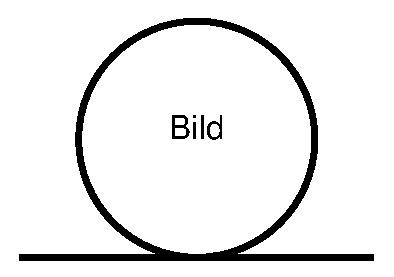
\includegraphics[width=0.48\textwidth,height=9cm]{beispiel}
%       \caption{Rechtes Beispielbild}
%       \label{fig:beispiel13}
%   \end{minipage}
% \end{figure}
% 
% Erw�hnenswert ist hier auch das Paket subfigure, das hier aber nicht besprochen wird.
% 
% \clearpage	% neue Seite einleiten, alle Gleitobjekte (Tabellen, Bilder) anzeigen
% \subsection{Bilder mit \LaTeX\ zeichnen}
% 
% Vektorbilder kann man auch direkt unter \LaTeX\ zeichnen. \\
% \textbf{Achtung!} Alles wird mit Hilfe von (ggf. skalierten) Textzeichen gezeichnet! Z.B. Kreise haben deswegen nicht umbedingt exakt die gew�nschte Gr��e. Die Grundeinheit deswegen am besten in Punkten (bei Schriftarten �blich) und nicht in mm o.�. angeben.
% 
% \setlength{\unitlength}{2mm}	% Einheit festlegen (Angabe in Punkten (pt) w�re besser, s.o.)
% \begin{figure}[h]
%    \centering	% zentrieren
%    \begin{picture}(10,10)	% Bild mit Gr��e (10,10) (Einheit s.o.)
%    	\put(0,0){\line(1,0){10}}	% Linie von (0,0) in Richtung (0,1) mit L�nge 10 ziehen
% 	\put(10,0){\line(0,1){10}}	% Linie von (10,0) in Richtung (0,-1) mit L�nge 10 ziehen
% 	\put(10,10){\line(-1,-1){10}}	% Linie von (0,10) in Richtung (-1,1) mit einer horzontalen L�nge von 10 ziehen
% 	\put(5,5){\circle{2}}	% Kreis bei (5,5) mit Durchmesser 2 ziehen
% 	\put(5,5){\circle*{1}}	% ausgef�llten Kreis bei (5,5) mit Durchmesser 1 ziehen
% 	\multiput(5,-1)(1,0){5}{\line(0,1){2}}	% Ein Objekt (hier Linie) mehrmals zeichnen: hier beginnend bei (5,-1) insgesamt 5 mal zeichnen immer um (1,0) versetzt.
% 	% viele andere Zeichenelemente sind ebenfalls m�glich 
%    \end{picture}
%    \caption{Eine mit \LaTeX\ gezeichnete Graphik}	% Bildbezeichnung
%    \label{fig:beispiel14}	% Interne Bezeichnung um Bild im Text referenzieren zu k�nnen
% \end{figure}
% 
% \clearpage
% \section{Fu�noten}
% 
% Fu�noten\footnote{Dies ist �brigens eine Fu�note} werden direkt an die Stelle geschrieben wo die Fu�notenzahl erscheinen soll. Kein Leerzeichen \footnote{Noch eine Fu�note} vorher machen, sonst erscheint dieses im Text. 
% 
% In Tabellen kann man das aber so leider nicht machen. Da mu� man die Fu�notenmarkierung manuell einf�gen und den Fu�notentext dann nach der Tabelle manuell angeben: \\
% 
% \begin{table}[h]
% \caption{Eine Tabelle mit einer Fu�note}
% \center
% \begin{tabular}{ccc}
% \hline
%  Name & Vorname\footnotemark & Sonstiges \\
% \hline
%  a & b & c \\ 
% \hline
% \end{tabular}
% \end{table}
% \footnotetext{Eine Tabellenfu�note}
% 
% Will man in einer Tabelle mehrere Fu�noten eintragen steht am Schlu� der Tabelle leider der Fu�notenz�hler an der letzen eingetragenen Fu�note. Um den Fu�notentext f�r die anderen Fu�noten angeben zu k�nnen mu� man diesen Z�hler vorher wieder zur�ckdrehen: \\
% 
% \begin{table}[h]
% \caption{Eine Tabelle mit mehreren Fu�noten}
% \center
% \begin{tabular}[c]{ccc}
% \hline
%  Name\footnotemark & Vorname\footnotemark & Sonstiges\footnotemark \\
% \hline
%  a & b & c \\ 
% \hline
% \end{tabular} 
% \end{table}
% 
% \addtocounter{footnote}{-3} % Anzahl der Fu�noten in der letzen Tabelle zur�ck
% \addtocounter{footnote}{1}\footnotetext{Die erste Tabellenfu�note} % Z�hler eins hochz�hlen und Text angeben
% \addtocounter{footnote}{1}\footnotetext{Die zweite Tabellenfu�note} % dito, f�r d�r die n�chste Fu�note
% \addtocounter{footnote}{1}\footnotetext{Die dritte Tabellenfu�note} 
% 
% \par
% \bigskip
% 
% Bei Fu�noten in Formeln mu� man das ebenfalls so machen. $ 1 + 1 =\footnotemark 2 $ 
% \footnotetext{Fu�noten in Formeln? Sind Sie verr�ckt?}
% 
% \bigskip
% 
% \newcounter{fn} % Neuen Z�hler erzeugen
% Um ein und die selbe Fu�note mehrmals im Text erscheinen zu lassen\footnote{Mehrmals erscheinende Fu�note}\setcounter{fn}{\value{footnote}} % Fu�notennummer im Z�hler speichern
% kann man das manuell\footnote{Das ist aber unsicher, da sich die Nummer beim Einf�gen von anderen Fu�noten �ndern kann} so\footnotemark[11] oder besser so\footnotemark[\value{fn}] % Fu�notenmarkierung mit dem gespeicherten Wert einf�gen.
% machen.
% 
% 
% \clearpage	% neue Seite einleiten, alle Gleitobjekte (Tabellen, Bilder) anzeigen
% \section{Mathematische Formeln}
% 
% F�r die Darstellung von Formeln mu� \LaTeX\ in den sog. {\em Mathematischen Modus} wechseln.
% Das geht in einen laufenden Text so: $ \int_a^b ( \exp (a \pi) ) da = \int\limits_a^b e^{a \pi} da $.
% 
% Freistehende Formeln macht man so:
% \begin{equation}
%  \sum\nolimits_{i=0}^{10} A = \sum\limits_{(i)}
%  A % Zeilenumbruch und Leerzeichen unwirksam
% \end{equation} 
% 
% Mehrere Formeln in einer Folge kann man so schreiben:
% 
% \begin{eqnarray}	% Zeilenumbruch wirksam!
%   D := \sqrt[n]{ \sin a \pi } \\
%   B := D^n \quad \Longrightarrow \quad B = \sin a \pi \\
%   E := 1 \nonumber \\	% keine Formelnummer anzeigen
%   \mbox{Eingef�gter Text} \nonumber \\ % Text mit mbox einf�gen
%   F := \frac{D}{B+E} \\
%   j^2 & = & -1  \\ % auch Ausrichtung mit & (wie in einer Tabelle) m�glich
%   \mbox{Sowas ist auch m�glich: $ \int \left( 2 \cdot \mbox{Haha} \right) $} % Mehrfach eingekapselte Umgebung
% \end{eqnarray} 
% 
% Gro�e Klammern macht man so:
% \begin{equation}
%  \left\lbrace \frac{1}{1+\frac{1}{1+\frac{1}{1+\frac{1}{1+\frac{1}{1+A}}}}} \right\rbrace 
% \end{equation} 
% 
% bzw. mit runden Klammern:
% \begin{equation}
%  \left( \frac{1}{1+\frac{1}{1+\frac{1}{1+\frac{1}{1+\frac{1}{1+A}}}}} \right)
% \end{equation} 



\chapter{Apps f�r Smartphones}

In diesem Kapitel 
		
		\section{Handykultur im heutigen Zeitalter}         
        Entwickelt wurde das Mobiltelefon, um auch unterwegs und nicht nur an
        station�ren Punkten Telefonate f�hren zu k�nnen. Doch bald war die
        Telefonfunktion nicht mehr die einzige bzw. relevanteste Funktion am
        Handy. 
        
        \begin{quote}
        ``Zur Erfindung der SMS als ``unbeabsichtigtes Nebenprodukt'' des
        Mobiltelefonierens kam es im Jahr 1992 eher zuf�llig, als einige
        Entwickler der Firma Vodafone sich einige noch �bersch�ssige
        �bertragungskapazit�t des Handy- Signalisierungskanals zunutze machten
        und �ber diesen eine Textnachricht mit dem Wortlaut ``Merry Christmas''
         an das Handy eines Kollegen verschickten.'' [Schmalenbach05], S. 3
%		  Anschlie�end wurde der
%         Versand von Kurzmitteilungen zun�chst ausschlie�lich von den
%         Netzbetreibern als Informationsdienst genutzt, um ihre Kunden �ber
%         eingegangene Nachrichten auf der Sprachmailbox zu informieren, bevor
%         der Short Message Service 1994 der �ffentlichkeit vorgestellt wurde
%         und ab 1996 die ersten SMS-f�higen Mobiltelefone f�r den privaten
%         Gebrauch den Siegeszug der SMS
%         einl�uteten.''
        \end{quote}

		Die Verbreitung des Handy nimmt weltweit immer mehr zu. Die von der ITU
		ver�ffentlichen Zahlen bewegen sich in unglaublichen Dimensionen: Von 6,1
		Billionen weltweit verschickten SMS im Jahr 2010 beziehungsweise von 200.000
		Kurzmitteilungen pro Sekunde ist die Rede. Das Handy wird f�r einen gro�en
		Teil der Weltbev�lkerung immer wichtiger. Die ITU sch�tzt die Zahl der am
		Jahresende 2010 vorhandenen Handyvertr�ge auf �ber 5 Milliarden. Dabei sind
		die Industrienationen f�hrend in der Handynutzung. [ITU10], letzter Abruf:
		30.11.2010
		
		Mobiltelefone haben bereits einen Riesigen Markt abgedeckt und trotzdem
		steigt die Nachfrage nach ihnen weiter an. Sie sind f�r uns Telefon,
		Organizer und/oder Spielekonsole in einem und bieten uns viele verschiedene
		Funktionen an, die vor noch nicht allzu langer Zeit nur auf Desktoprechnern
		ausf�hrbar waren. Im Schnitt werden Handys nach 12 bzw. 24
		Monaten durch ein neues Modell ersetzt (Durchschnittliche Vertragslaufzeiten).
		Die Industrie �berrascht uns immer wieder mit neuen Technologien und
		Innovationen innerhalb k�rzester Zeit. %Doch
		%wohin f�hrt uns dieser rasende Wechsel? evtl. kleiner Ausblick? aber worauf?
		
		Es gibt viele Konzepte von Mobiltelefonen und wie diese in der Zukunft
		aussehen k�nnten. Entw�rfe mit den verschiedensten Materialien sollen Handys
		flexibler machen oder neue Formen von Design aufzeigen(Vgl. Abbildung
		\ref{fig:handy1} und \ref{fig:handy2}).
		
		\begin{figure}
		  \begin{minipage}[t]{0.48\textwidth}	% Minipage erzeugen, [t] = Am oberen Rand ausrichten
		      \centering	% zentrieren
		      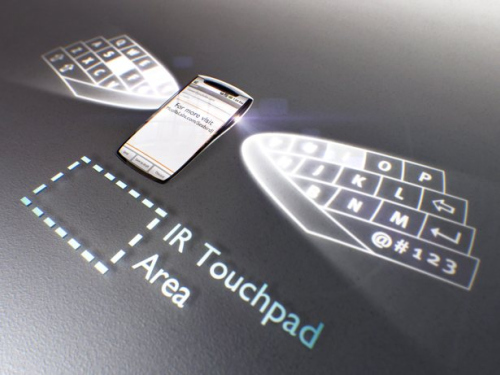
\includegraphics[width=1\textwidth]{handy1}
		      \caption{Concept Phone 1}
		      \label{fig:handy1}
		  \end{minipage}% (kein horiz. Abst. zw. minipages)
		  \begin{minipage}{0.04\textwidth}
		     \hfill % Damit die getrennte Beschriftung auch Abstand hat
		  \end{minipage}%
		  \begin{minipage}[t]{0.48\textwidth}
		      \centering	% zentrieren
		      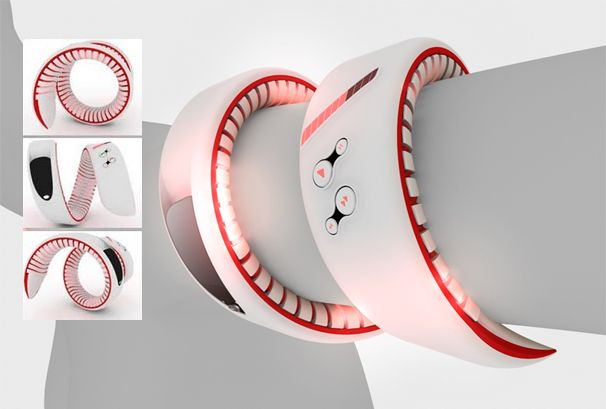
\includegraphics[width=1\textwidth]{handy2}
		      \caption{Concept Phone 2}
		      \label{fig:handy2}
		  \end{minipage}
		\end{figure}
%Quelle angeben?
% http://www.computerworld.com/s/article/9176806/20_crazy_concept_phones?taxonomyId=75&pageNumber=2

		
		Ein Interessanter Ansatz scheint es zum Beispiel zu sein, den Menschen quasi
		auch als ``Hardware'' in das Mobiltelefon zu integrieren (Vgl. Abbildung \ref{fig:handy3}).
		Beim ``Finger Whisper'' beispielsweise erzeugt ein Terminal am Handgelenk aus
		Sprachinformationen Schallwellen, die �ber das Handgelenk weitergegeben.
		Diese Schallwellen k�nnen dann �ber den Zeigefinger ans Ohr gelangen, um so
		wieder zu verst�ndlicher Sprache zu werden. [CHI99]
		
		\begin{figure}
		  %Rand ausrichten 
		  \centering	% zentrieren
		      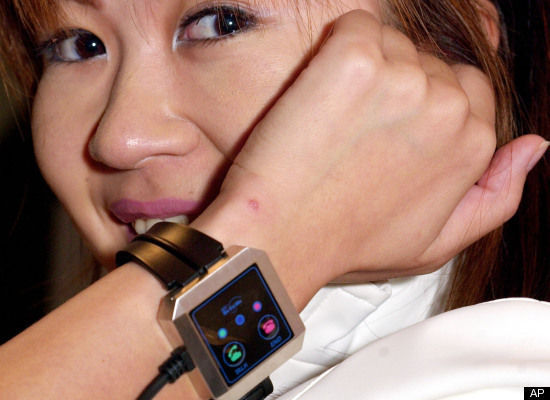
\includegraphics[width=0.48\textwidth]{handy3}
		      \caption{Finger Whisper}
		      \label{fig:handy3}
		\end{figure}
		
		Die KHS m�chte im Rahmen dieser neuen Technologien Anschluss finden, um
		moderne Konzepte in der Firma einzuf�hren und diese f�r die
		Produktion/Weiterentwicklung von Fertigungsmaschinen zu nutzen. Der Erfolg
		von modernen Mobiltelefonen und deren Verbreitung hat gro�es Potenzial, was
		die Wachstumsraten im Verkauf best�tigen. Dieser Markt soll im Rahmen der
		M�glichkeiten genutzt werden, um die KHS Linie entsprechend zu erweitern.
        
	\section{Definition App}
	Es sind viele Definitionen von ``App'' im Internet zu finden. Auch wenn das
	iPhone sehr viel zur Popularit�t von Apps beigetragen hat, hat Apple diese nicht
	erfunden. Nicht umsonst verzeichnet der Apple App Store, die zentrale
	Anlaufstelle f�r Anwendungen f�r das iPhone und den iPod Touch, bereits �ber sieben
	Milliarden Programm-Downloads. [Apple10], letzter Abruf
	30.11.2010

	``App'' steht f�r Application, sprich die Anwendung und
	bedeutet erstmal auch nichts weiter als das. In Kombination von mobilem
	Endger�t (Smartphone) und einer darauf laufenden Anwendung spricht man daher
	vom ``App''.

	Der Nutzen einer solchen l�sst sich wie folgt kurz beschreiben: Eine App soll
	dem Anwender neue Funktionen in Form von Programmen, wie z.B. Spielen oder
	Anwendungen auf seinem mobilen Endger�t zur Verf�gung stellen. Dabei gibt es
	Apps, die rein auf den Spa�-Faktor abzielen, andere wiederum k�nnen dem
	Nutzer schnell wertvolle Informationen bereitstellen wie Ausgehtipps mit
	Restaurant- und Veranstaltungsinformationen, Wetteraussichten, aktuelle
	Wechselkurse oder die g�nstigste Tankstelle. 
	
	Als Marketinginstrument wurden die Apps inzwischen auch von Unternehmen
	gezielt eingesetzt, um ihre Marke erlebbarer zu machen und
	emotional aufzuladen. So gibt es beispielsweise von Pizza Hut eine App, mit dem man sich
	mit wenigen Klicks seine Lieblingspizza zusammenstellen und
	bestellen kann. Der Vorteil: Man kann von unterwegs die Pizza bestellen und
	so Zeit sparen. Mit im App enthalten ist zudem der Pizza Hut Racer, ein
	Autorennen-Spiel - der beim (potentiellen) Kunden f�r jede Menge Spa� sorgen
	soll. So wird der Kunde an die Marke gebunden.
	
	%Konkret f�r die KHS umgesetzt k�nnte das heissen, dass man mit einer neuen
	%Produktlinie Kunden gewinnt und/oder bestehende Kunden an die Firma bindet.
	%TODO: m�glicher Nutzen f�r die KHS /allgemeiner Maschinenbau... hmpf..
	
	
	
	\section{Funktionsumfang und Nutzen seitens der KHS}

		%\section{Konzept f�r die zu entwickelnde/n App/Apps}                                                                                                                                                                                                                                                                                                                                                                
			\subsection{Zielsetzung}
			Nachfolgend werden spezielle Ziele, die die KHS GmbH mit der Erstellung
			einer Smartphone App erreichen m�chete, vorgestellt.
                
            \subsection{Wirtschaftliche/Marketingtechnische Erw�gungen}
			            
            Dank der intuitiven Bedienkonzepte von Smartphones ist es m�glich
            sehr benutzerfreundliche Umbegungen zu schaffen. Jeder, der bereits
            ein Smartphone bedient hat kennt die auf Touchscreens eingesetzten 
           	Techniken, um Symbole zu manipulieren. Somit werden intuitiv
           	Oberfl�chen, die sich an diese Richtlinien der Smartphones halten,
           	vom Benutzer richtig erfasst und angenommen. Eine l�ngere
           	Schulungsma�name, um mit der Bedienung arbeiten zu k�nnen entf�llt
           	logischerweise. [Clark10], S. 11ff
            
            Ebenfalls f�r die Entwicklung auf mobilen Endger�ten spricht, dass
            viele Mitarbeiter von Firmen bzw. Kunden schon ein Smartphone
            besitzen. Somit entstehen keine bzw. nur geringe Zusatzkosten f�r
            die anzuschaffende Applikation beim Kunden. Dies macht den BLA
            unter Kostengesichtspunkten sehr attraktiv, da die Hardware f�r das
            Produkt schon vorhanden ist.
            
            Durch die Unabh�ngigkeit zum Maschinenstandort wird die
            Flexibilit�t mit dem Umgang der Maschine erh�ht. Beispielsweise
            sollen verschiedene Basisfunktionen auch �ber die Smartphone App
            zur Verf�gung gestellt werden. Der Mitarbeiter muss also nicht
            direkt bei der Maschine sein, um diese zu bedienen oder zu warten.
            Dies verschafft dem Kunden einen Zeitvorteil, der eine
            Kostenersparnis nach sich zieht, weil Abl�ufe schneller erledigt
            werden k�nnen.
            
            Eventuell l�sst sich auch die Kommunikation der Mitarbeiter
            untereinander durch Smartphone Applikationen verbessern.
            Vorstellbar w�re hier, dass Nachrichten bzw. Protokolle �ber die
            App ausgetauscht werden k�nnen oder auch direkt die Nummer der
            zust�ndigen Hotline anw�hlbar ist, falls eine R�ckmeldung der
            Maschine das erfordert.
             
			Durch die Unterst�tzung von neuen Technologien, die dem Kunden Zeit- bzw.
			Kostenvorteile bieten werden von KHS hergestellte Maschinen deutschlich
			attraktiver als Maschinen von Mitbewerbern, die nicht �ber die gleiche
			Funktionalit�t verf�gen.
            
           	Solche vergleichsweise einfach zu erstellenden Applikationen mit
           	wenigen Grundfunktionen pro App (evtl. viele Verschiedene; hohe
           	Skalierung) k�nnen beim Kunden neue W�nsche wecken. Die
           	M�glichkeiten sind hier sehr weitreichend. Deshalb k�nnte es durch
           	die Akzeptanz beim Kunden und die rasche Verbreitung von
           	anf�nglichen Apps zu einer neuen Produktlinie bei KHS f�hren, wenn
           	die Nachfrage gro� genug ist.
			
			Corporate Identity (kurz CI) stellt den abgestimmten Einsatz von Verhalten,
			Kommunikation und Erscheinungsbild nach innen und au�en dar. Basis ist
			das Unternehmensleitbild, welches mit Leben gef�llt wird. Die CI ist also die
			Pers�nlichkeit einer Organisation. Smartphone Applikationen haben
			mittlerweile einen relativ hohen Stellenwert in der modernen Gesellschaft
			erreicht. Mit einem gelungenen Einstieg in diesen Bereich w�re eine
			positive Au�enreaktion und dadurch eine Ausweitung des Leitbildes der KHS
			m�glich im Sinne eine Imagegewinns in der �ffentlichkeit.
            

			\subsection{Funktionsumfang}
			Konkrete Funktionen, die f�r Apps denkbar sind sehen wie folgt aus:
			
			\begin{itemize}
              \item Teaching: Bei der Inbetriebnahme einer Fertigungsmaschine
              soll es m�glich sein ein Video zu streamen, welches erkl�rt wie
              die Maschine eingerichtet wird. Weiterhin sollen unterst�tzende
              Videos dem Nutzer durch Abruf erm�glichen, bei einfachen
              Fehlermeldungen der Maschine diese durch Anleitung zu beheben.
              Dazu werden kurze Videoausschnitte gezeigt, die die einzelnen
              Schritte f�r den Benutzer verst�ndlich erkl�ren. Durch Bet�tigung
              eines Buttons wird von Schritt zu Schritt gewechselt.
              \item Messaging: Es soll dem Nutzer der Applikation erm�glicht
              werden einfache Meldungen und/oder Notizen an die Visu-Station zu
              schicken bzw. Meldungen zu empfangen. % und Notizen
              \item Push Notification: Verschiedene Zust�nde der Maschine
              sollen dem Nutzer als Nachricht �bermittelt werden k�nnen. Diese
              werden allerdings nicht vom Nutzer abgerufen sondern von der
              Maschine auf das Ger�t ``gepusht''. Dabei sind Fehlermeldungen
              genauso denkbar wie andere Nachrichten, z.B. wenn eine Maschine
              einen vorher festgelegten Richtwert �berschreitet.
              \item Monitoring: Die Produktion und der Durchlauf der Maschine
              soll am Ger�t live angezeigt werden. M�gliche Datens�tze
              sind hier Auslastung der Maschine, umbauzeiten, Dauer von
              Wartungsarbeiten, etc. % evtl. in Kombination mit vorletztem
              %Punkt -> Anzeige von Einzelaggregaten
              \item Reporting: Aktuelle Statistiken der Produktionsdaten in Form
              von Reports sollen vom Nutzer abrufbar sein. So k�nnen
              Echtzeitdaten beispielsweise in Pr�sentationen oder bei
              Besprechungen verwendet werden (Anzeige auf dem Smartphone oder
              Versand per Email auf Anforderung denkbar).
              \item Control: Es soll durch den Benutzer m�glich sein
              unkritische Funktionen der Maschine zu steuern (m�gliche Fehler
              durch den Benutzer in der Bedienung m�ssen ausgeschlossen werden).
              \item Bug-Reporting: Es soll m�glich sein Maschinenfehler an den
              Server zu schicken, um diese dem Support zur Verf�gung stellen zu
              k�nnen. Dies soll durch eine manuelle Eingabe in einem
              Fehlerberichtsformular m�glich sein. Zus�tzlich denkbar ist es,
              dass mit der Kamera am Smartphone ein Foto des Defekts mit dem
              Bericht mitgesandt wird.
              \item View: Einzelaggregate mit Ihren verschiedenen Stati sollen
              abfragbar sein. Dabei handelt es sich um Aggregate der Maschine,
              die normalerweise nicht am Maschinendisplay auftauchen und f�r
              spezielle Operationen ben�tigt werden (Beispielsweise bei
              Inbetriebnahme oder St�rungsbeseitigung).
              \item Spare Parts Catalogue: In einem �ber Smartphone aufrufbaren
              Ersatzteilkatalog soll es m�glich sein, Teile der verwendeten
              Maschine nachzubestellen. Bei einem Fehler wird von der Maschine
              �berpr�ft, ob ein Maschinenteil defekt ist. Falls dies zutrifft,
              wird dem Benutzer vorgeschlagen, dieses nachzubestellen.
              %(Kamera?)
            \end{itemize}

%			\begin{itemize}
% 	          \item Personenbezogene Aufgabenverteilung (Taskliste)  von einer
% 	          zentralen Taskverwaltung (z.B. Reperaturauftr�ge) anzeigen und
% 	          bearbeiten (in Arbeit, fertig, weiterleiten...). Eventuell Sync
% 	          mit Google Calender m�glich. Aber erstrebenswert?
%	        \end{itemize}

\section{Sicherheit in mobilen Netzen}
            
            \subsection{Sicherheitsprobleme in mobilen LANs und WANs}
            \begin{quote}
            ``Funknetze haben im Gegensatz zu leitungsgebunen Netzen
            zus�tzliche Gef�hrdungspunkte, die zumeist aus den verwendeten
            �bertragungsprotokollen und der nur begrenzt kontrollierbaren
            Ausbreitung der Funkwellen ergeben.'' [Eren06], S. 259
            \end{quote}

			\subsubsection{Bluetooth}
			
			Bluetooth erm�glicht die drahtlose Daten�bertragung und l�sst sich dabei
			leichter konfigurieren als Beispielsweise WLAN. Es wird dabei kein direkter
			Sichtkontakt zwischen den beteiligen Ger�ten ben�tigt (vgl. IRDA).
			
			%\subsubsection{Designschw�chen und Implementierungsschw�chen}
			
			In der Spezifikation von Bluetooth wird kein Verschl�sselungsalgorithmus
			vorgeschrieben, deswegen ist in der Standardkonfiguration vieler Hersteller
			die Verschl�sselung ausgeschaltet. Aber auch wenn diese aktiviert sein
			sollte, heisst dies nicht unbedingt, dass die Verbindung sicher ist.
			Der Verschl�sselungsalgorithmus bei Bluetooth baut auf einer XOR-Verkn�pfung
			von Klartext und Schl�sselstrom auf. Ein Angreifer kann Teile der
			versendeten Nachricht herausfinden, weil der zur Kommunikation benutzte
			TCP/IP-Header eine bekannte Form hat (hinsichtlich Gr��e und Aufbau).
			Als Folge sinken m�gliche Schl�sselkombinationen (Reduktion der
			effektiven Schl�ssell�nge von 128 Bit auf 84 Bit wegen des bekannten
			Headers). ``Brute-Force''-Angriffe werden somit erleichtert.
			
			Ein anderer Ansatzpunkt f�r Angreifer stellt der Zufallszahlengenerator dar.
			Zufallszahlen werden in einigen Sicherheitsfunktionen verwendet. In der
			Spezifikation des Bluetooth-Standards werden keine expliziten Anforderungen
			an diesen gestellt. Da verschiedene Hersteller wirtschaftlich g�nstige
			Algorithmen w�hlen, k�nnen teilweise durch die Bekanntheit dieser
			Algorithmen die Ergebnisse vorhergesagt werden.
			
			Der bei einer Authentifizierung notwendige vierstellige Pin-Code stellt auch
			bei einer 128-Bit Verschl�sselung leider immer noch keine ausreichende
			Sicherheit zur Verf�gung. Im Auslieferungszustand des Ger�ts ist
			dieser meist auf ``0000'' gesetzt. Wenn der Pin-Code vom Angreifer also
			richtig ermittelt werden kann, hat er die M�glichkeit die Kommunikation von
			gepairten Ger�ten ungest�rt zu belauschen.
			
			Alle Sicherheitsdienste bei Bluetooth sind in der Daten�bertragungsschicht
			(Schicht 2 des ISO-OSI-Schichtenmodells) angesiedelt. Somit gibt es keine
			Ende-zu-Ende Sicherheit. Die Verbindung wird zwar verschl�sselt, aber es
			fehlt eine nahtlose und durchgehende Datenverschl�sselung zwischen den
			Endger�ten.
			
			Das OBEX-Protokoll wird vor allem bei Bluetooth-Push-Diensten
			eingesetzt. Auch dieses hat Schw�chen. Der Stack wird vom
			Zulieferer und nicht vom Hersteller implementiert. Somit kann es passieren,
			dass Bluetooh-Ger�te, die den gleichen Stack und das gleiche virtuelle
			Dateisystem besitzen unauthorisierte Zugriffe aufs Filesystem (z.B.
			Telefonbuch) unbeabsichtigt offen legen.
			
% 			Spoofing. Vort�uschen falscher Identit�t. Ger�t A kommuniziert mit B. Ger�t
% 			C mit A und B. B nimmt Identit�t (Link Key) von C an und t�uscht diesen bei
% 			A vor. Kommunikation belauschen? Seite 270...
			
% 			Bluesniping mit Richtantenne. Bluetooth-Ger�te m�ssen normalerweise in
% 			unmittelbarer Reichweite sein (ca. 10 Meter entfernt). Mittels der
% 			Richtantenne lassen sich auch weit entfernte Ger�te  angreifen (bis zu 1
% 			Kilometer).
					
			\subsubsection{GSM}
						
			GSM wurde auf Basis der bereits bestehenden Festnetztechnik entwickelt. Die
			Verschl�sselung der Daten wurde nur als Option definiert, da in einigen
			L�ndern eine Verschl�sselung von staatlicher Seite untersagt ist. Auch wird
			auf den meisten Endger�ten nicht angezeigt, ob eine Verbindung verschl�sselt
			ist oder nicht. Ein weiterer Schwachpunt stellt der Umstand dar, dass Daten
			nur zwischen der BTS und dem Teilnehmer verschl�sselt werden. Das abh�ren
			von diesen Verbindungen ist an den diversen Schnittstellen der BTS zu
			anderen Netzkomponenten ohne gro�en Aufwand m�glich. Der potentielle
			Angreifer verschafft sich physischen Zugang zu einem BTS und kann von dort
			die Kommunikation belauschen bzw. manipulieren.
			
			Ebenfalls eine Schwachstelle ist der Kurznachrichtendienst SMS. Hier werden
			Nachrichten unverschl�sselt �ber den Signalisierungskanal �bertragen. Anhand
			der �bertragungsfrequenz kann so ein Angreifer Nachrichten mitlesen.
			
			\subsubsection{GPRS}
			
			GPRS stellt eine Erweiterung des GSM-Netzes um paketorientierte
			Daten�bertragung dar. Der Einstieg �ber das GPRS-Netz ins Internet wird als
			$G_{i}$-Schnittstelle bezeichnet. W�hrend der Datenkommunikation �ber GPRS
			ist der Teilnehmer anf�llig f�r im Netz verbreitete Gefahren und Angriffe.
			Falls der Datenverkehr unverschl�sselt stattfindet besteht die Gefahr, dass
			Daten durch einen Angreifer abgefangen und missbraucht werden. H�ufig
			rechnen Mobilfunkbetreiber mit solchen Gefahren und platzieren eine Firewall
			an der $G_{i}$-Schnittstelle.
			
			\subsubsection{UMTS}
			
			UMTS stellt eine Erweiterung auf Basis der verbreiteten Technik dar. Damit
			gew�hrleistet ist die Abw�rtskompatibilit�t zu GPRS/GSM. Prizipiell ist diese
			Technologie anf�llig f�r Denial-of-Service- und Impersonationsattacken. Unter
			Impersationsattacken versteht man die Verwendung eines kompromittierten
			Authentisierungsvektors, um sich unter der Identit�t des wahren Teilnehmers
			an das Netz anzumelden.
			
			%TODO: hier weiterschreiben!!!
			
			\subsubsection{HSDPA}
			
			fehlende info... buch zu alt. evtl. auf quelle im internet verweisen.
			
			\subsubsection{LTE}
			Neue Technik!!! noch nicht in Deutschland verf�gbar...
			
			\subsubsection{Wireless LAN}
			
			Die Mit der technischen Spezifikation verbundene Systemoffenheit
			zuverl�ssige und bequeme Einstiegspunkte ins ein Netzwerk zur Verf�gung zu
			stellen enbl��t leider auch abgeschottete private Netzwerke. Im Folgenden
			werden die verschiedenen Methoden der Verschl�sselung f�r Wireless LAN (kurz
			WLAN) erl�utert und konkret auf deren Schwachstellen eingegangen.
			
			\subsubsection{WEP}
			
			Das WEP-Protokoll verwendet zur Absicherung der Verbindung den symmetrischen
			Algoritmus RC4. 
			
			\begin{quote}
           	``Dieser ist ein Stromverschl�sselungsalgorithmus, der den
			Klartext �ber eine XOR-Operation mit einer Folge von Pseudozufallszahlen
			verkn�pft.'' [Eren06], S. 287
			\end{quote}
			
			Der WEP-Key wird entweder mit 40 Bit (WEP 64) oder 104 Bit (WEP 128) erzeugt.
			
			%\subsubsubsection{Schw�chen von WEP}
			
			%Schw�chen von WEP
			
			Schlechte Implementierungen des Initialisierungsvektors (der zusammen mit
			dem WEP-Key dazu benutzt wird die �bertragung zu verschl�sseln) f�hren zu
			Kollisionen in den �bertragenen Daten. Angreifer k�nnen diese Kollisionen
			erkennen und dadurch auf die unverschl�sselte Nachricht schliessen.
			
			Bei WEP fehlt eine gegenseitige Authentisierung. Aufgrund der Einfachheit,
			eine Netzwerkkomponente (insbesondere MAC-Adresse) zu f�lschen entsteht
			damit eine wesentliche Sicherheitsl�cke.
			
			Nach RFC 1024 m�ssen alle IP- und ARP-Pakete stest mit einem ``0xAA'' beginnen.
			Dies kann von einem Angreifer ausgenutzt werden, um den WEP-Schl�ssel zu
			ermitteln. Mit relativ wenig Aufwand wird genug Chiffretext gesammelt. Um
			den Schl�ssel ermitteln zu k�nnen, m�ssen die ersten Bystes des Klartextes
			bekannt sein. Aufgrund der Anforderung nach RFC haben Angreifer also
			leichtes Spiel.
			
			
			
			\subsubsection{WPA}
			
			Der grundlegende Unterschied zu WEP ist die Verwendung von TKIP als
			Verschl�sselungsprotokoll. Prinzipiell l�sst sich WEP mittels Software- und
			Firmware-Updates auf WPA upgraden.
			
			Um die Schwachstellen von WEP auszumerzen implementiert WPA dynamische
			Schl�ssel f�r jedes versendete Paket. Dabei besitzt jeder Benutzer einen
			eigenen Schl�ssel.
			
			WPA ist anf�llig f�r W�rterbuchattacken, da der Preshared Master Key direkt
			aus der Passphrase und der SSID abgeleitet wird. F�r einen solchen Angriff
			reicht ein aufgezeichneter TKIP-Handshake aus. Allerdings ben�tigen die
			anschlie�enden Berechnungen einen aktuellen High-End-PC, da gerade einmal
			ca. 70 Passw�rter pro Sekunde gepr�ft werden k�nnen. Falls also ein
			geeignetes starkes Passwort gew�hlt wurde geht von dieser Attacke eine nur minimale
			Gefahr aus.
			
			\subsubsection{WPA2}
			
			Da der bei WEP und WPA zugrundeliegende Algorithmus RC4 als gebrochen gilt,
			wurde bei WPA2 die AES Verschl�sselung eingesetzt. Dabei bleibt WPA2 noch zu
			WPA abw�rtskompatibel.
			
			Eine ``Brute-Froce''-Attacke ist zwar rein theoretisch denkbar, aber sehr
			unwahrscheinlich, da die Wahrscheinlichkeit f�r eine identische Pr�fsumme
			eines MAC bei ca. 1 : 1 Mio. liegt. Ausserdem wird bei einer Attacke ein 60
			Sekunden andauernder Blackout (Unterbrechen der Verbindung) des Access
			Points verwendet, um etwaige Attacken abzublocken. Allerdings kann eine
			``Denial-of-Service''-Attacke so durchaus erfolgreich sein, wenn es der
			Angreifer nicht auf den Schl�ssel abgesehen hat.
            
            \subsection{Denkbare Angriffsformen auf Mobiltelefone in einer
            Firmeninfrastruktur}
            
            \begin{itemize}
	            \item Aussp�hen von Daten: Der Angreifer verschafft sich
	            Zugang zu relevanten Daten, die auf dem jeweiligen Ger�t
	            gespeichert sind. Dazu geh�ren Kontaktlisten, E-Mails, SMS und
	            andere vertrauliche Dokumente und Dateien.
	            \item Nutzung eigener Dienste und Zug�nge: Wird eine
	            Authentifizierung lediglich beim Einschalten des Ger�ts verlangt,
	            kann das Ger�t im Verlustfall ganz leicht von Kriminellen wie ein
	            Schl�ssel f�r Dienste und Zug�nge genutzt werden. Dadurch k�nnen
	            Sicherheitsmechanismen, die Firmen-, Service- oder Datenstrukturen
	            vor unbefugtem Zugang sch�tzen, ausgehebelt werden.
	            \item Manipulation der Software-Komponenten: Dabei k�nnen Angriffe
	            auf Netzwerke in Verbindung mit der Synchronisation zwischen
	            mobilem Ger�t und dem Firmennetz erfolgen, um Informationen oder
	            Daten direkt zu erhalten. Dar�ber hinaus bietet die Konfiguration
	            von Proxies, die bei der Internetkommunikation genutzt werden, die
	            M�glichkeit des Abh�rens und Aufzeichnens, aber auch der
	            Manipulation (Tracing, Capturing, Logging) der an das Ger�t
	            zur�ckgesendeten Informationen.
	            \item �berwachung: Moderne Smartphones bieten neben
	            Kommunikationsschnittstellen wie GPRS, 3G, WLAN und Bluetooth
	            unl�ngst auch GPS-Module. Damit lassen sich raumbezogene
	            Referenzinformationen ablegen, die das Erstellen eines genauen
	            Bewegungsprofils erm�glichen. Dazu ist eine Manipulation des
	            Ger�ts notwendig, die aber keines Diebstahls bedarf.
            \end{itemize}
            
            \subsection{Sicherheitsmechanismen}
            
            Folgende Mechanismen sollen dazu beitragen, dass Firmenrelevante
            Daten nicht einfach von Dritten ausgesp�ht werden k�nnen.
            
            \subsubsection{WLAN sichern mit Radius}
            Beim WLAN-Einsatz in Unternehmen reicht die simple
            Authentifizierung �ber ein gemeinsames Passwort (Shared Secret)
            mit WPA-PSK nicht: Das Geheimnis ist bei gro�er Verbreitung zu
            schnell keines mehr. Sp�testens wenn ein Kunde vor�bergehend einen
            Zugang bekommen hat, muss man es �ndern. Mit serverseitig
            zugeteilten Passw�rtern erspart sich der Administrator viel Arbeit
            und Nachfragen seiner Nutzer.
            
            F�r solche Einsatzf�lle ist die Spielart WPA Enterprise gedacht,
            bei der die WLAN-Basisstation Verbindungsanfragen von ihren
            Clients �ber das Protokoll IEEE 802.1x mit einem nachgelagerten
            Radius-Server aushandelt. Auf Linux-Systemen ist dazu das
            Open-Source-Paket Freeradius g�ngig. [Radius10], letzter Abruf
            07.12.2010
            
            Mit dem Extensible Authentication
            Protocol (EAP) unterst�tzt es verschiedene kryptografisch
            gesicherte Methoden (EAP-TLS/-TTLS, PEAP, LEAP),
            One-Time-Passworte und SIMs. F�r die Authentifizierung sind
            Username/Passwort-Kombinationen oder Zertifikate gebr�uchlich.

			Damit Daten nicht im Klartext durch die Luft beziehungsweise �ber die
			Leitung zwischen Basisstation und Radius-Server laufen, verschl�sselt
			Freeradius diese. Voraussetzung daf�r ist, dass auf dem Client mindestens ein
			Stammzertifikat (Root CA Certificate) installiert ist, von dem das Zertifikat
			des Radius-Servers abgeleitet ist. Mit dem Stammzertifikat pr�ft der Client
			auch, dass er sich beim richtigen Radius-Server authentifiziert.
			
			\subsubsection{MDM}
			
			\begin{figure}
			  %\begin{minipage}[b]{0.48\textwidth}
			      \centering	% zentrieren
			      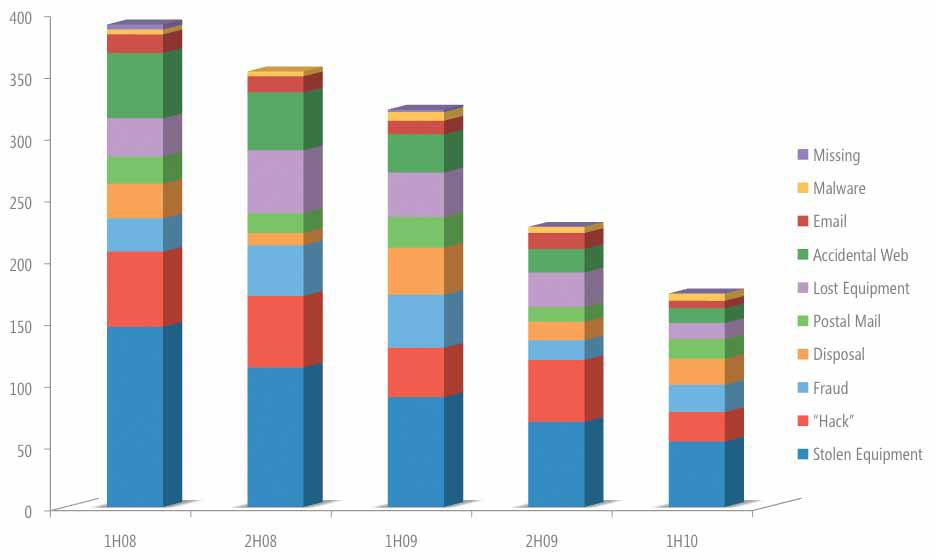
\includegraphics[width=0.8\textwidth]{microsoft_security_trends}
			      \caption{Datenverluste in Unternehmen}
			      \label{fig:microsoft_security_trends}
			\end{figure}
%TODO: Quelle
			
			
			Wie man der Abbildung \ref{fig:microsoft_security_trends} entnehmen kann
			f�hrt der Diebstahl von Endger�ten am h�ufigsten zu Sicherheitseinbr�chen in
			Systemen.
			
			MDM (Mobile Device Management) bezeichnet die M�glichkeit von der Ferne aus
			auf ein Mobiltelefon zuzugreifen und dieses gegebenenfalls zu sperren bzw.
			Daten zu l�schen oder andere Sicherheitsmechanismen auszul�sen.
			
			Die derzeitige Funktionspalette umfasst: 

			\begin{itemize}
              	\item auf dem Ger�t enthaltene Daten sichern und wieder
              	aufspielen (``Backup \& Restore'')
              	\item Software-Updates zentralisiert und drahtlos aufspielen, um
    			Sicherheitsl�cken schnell zu schlie�en (``Update Over The Air'')              
    			\item ein gestohlenes oder verlorenes Ger�t aus der Ferne sperren und
    			seine Daten l�schen (``Remote Lock \& Wipe'') sowie per GPS verfolgen
    			(``Mobile Tracking'')
    			\item einzelnen Nutzern differenzierte Rechte zuteilen - vom
    			Internet-Zugang bis zur Installation von Programmen (``Policy \&
    			Provisioning'')
    			\item  Statistiken erstellen, wie ein Smartphone genutzt wird und welche
    			Kosten anfallen (``Logging \& Accounting'')
            \end{itemize}

			Bei den MDM-L�sungen bekommen die Ger�te eine Identit�t zugewiesen, die mit den
			entsprechenden Zugangsberechtigungen und Funktionseinschr�nkungen verkn�pft ist.
			Im Idealfall bekommt der Nutzer f�r sein Smartphone nur noch ein Passwort, mit
			dem er sich einmalig f�r die Erstkonfiguration anmelden kann. W�hrend der
			normalen Nutzung im Alltag k�nnen die Firmen-Administratoren mittels MDM dann
			zentral Software-Updates verteilen, Ger�te sperren oder durch
			Konfigurations�nderungen schnell auf Sicherheitsl�cken reagieren. Wird das
			Smartphone schlie�lich ausgemustert oder verl�sst der Nutzer das Unternehmen,
			werden mittels MDM Berechtigungen gel�scht, Unternehmensdaten getilgt oder die
			Konfiguration auf ein neues Endger�t �bertragen.
									
			Der Markt f�r MDM-L�sungen ist derzeit noch �bersichtlich. Statistiken �ber
			Marktanteile existieren nicht. Zu den gro�en drei, die immer wieder genannt
			werden, geh�ren jedoch die US-Unternehmen Mobile Iron, Good Technology und
			Sybase. Ihre Produkte unterscheiden sich dabei vor allem im Detail - w�hrend
			Good Technology gro�es Know-how in Sales-Umgebungen verspricht, streicht man bei
			Mobile Iron die Handhabbarkeit unterschiedlicher Smartphone-Plattformen heraus.
			Sybase wirbt wiederum mit einer guten Anbindung an die hausinterne IT. Zumeist
			bezahlen Unternehmen einen Sockelbetrag plus eine Lizenzgeb�hr pro Nutzer. Mit
			insgesamt einigen Tausend Euro pro Jahr m�ssen die Firmen dabei rechnen.
			Anbieter wie Mobile Iron haben f�r Neukunden aber auch Lockofferten von nur vier
			Dollar pro Nutzer und Monat (plus Sockelbetrag) im Angebot.
									
			Was die Sache noch komplizierter macht: In vielen Firmen werden l�ngst nicht
			mehr nur reine Businessger�te wie die Blackberrys des kanadischen Anbieters RIM
			eingesetzt. Apples iPhone beispielsweise hat mittlerweile ebenfalls einen
			Siegeszug in Unternehmen angetreten. Der traditionsreiche IT-Dienstleister
			Unisys etwa, der f�r Firmen und Regierungen auf der ganzen Welt arbeitet,
			benutzt iPhones, um Server zu �berwachen, aber auch f�r h�chst
			sicherheitskritische Anwendungen wie die Steuerung von Systemen zur
			Kamera�berwachung.
									
			Ein weiterer kritischer Punkt sind private Anwendungen auf Firmen-Smartphones.
			Ger�te wie das iPhone laden geradezu dazu ein, neben gesch�ftlichen Apps auch
			Spiele zu installieren oder Multimedia-Content zu konsumieren. Schlie�en l�sst
			sich dieses Sicherheitsloch derzeit nur, indem Firmen das Aufspielen    privater
			Inhalte ganz verbieten.
			% TODO: �berarbeiten/umschreiben... evtl. streichen
            
            \subsection{Entscheidung f�r �bertragungstechnik}
            
            % evtl. bluetooth lt. gespr�ch?
            
          begr�ndung durch schlussvolgerung aus sicherheitsl�cken und
          erl�uterung sicherheitskonzept, damit die schwachstellen der technik
          nicht ausgenutzt oder nur zum teil ausgenutzt werden k�nnen.
           	
          \texttt{YASA} soll m�glichst unabh�ngig vom Standort genutzt werden
          k�nnen. Eine solche Flexibilit�t l�sst sofort einige der
          angesprochenen �bertragungstechniken ausscheiden. Die einzige
          M�glichkeit zu garantieren, dass die Applikation wirklich
          Standortunabh�ngig genutzt werden kann ist die Verwendung
          providerabh�ngigen Netzen. F�r WLAN, Bluetooth \& Co. muss das Ger�t
          immer in Reichweite mit der Empf�ngerstation bleiben, deswegen fallen
          diese weg.
          
          Fallunterscheidung: 
          
          Bei Funktionen, die nahe an der Maschine ausgef�hrt werden (z.B.
          Teaching) ist es denkbar, dass eine der Reichweite nach begrenzte
          Technik gew�hlt werden kann, um das Smartphone mit der
          Fertigungsmaschine zu koppeln.
          
          
          Apps, die unabh�ngig vom Standort funktionieren sollen(z.B.
          Reporting) m�ssen mit einer Verbindungstechnik ausgestattet werden,
          die auf ein WAN zugreifen kann.
          

\section{Gegenargumente ? umformulieren}
	warum keine apps in der industrie einsetzen?
	gefahr?
	bedienfehler?
	robustheit der ger�te?
	
	

\chapter{Grundlagen f�r die folgenden Kapitel}
F�r das Verst�ndnis der nachfolgenden Kapitel werden kurz wichtige Verfahren
benannt und Techniken beschrieben, die Anwendung finden. Weiterhin werden
Hinweise zu weiterf�hrender Literatur gegeben.

\section{MDA}

	In der Vergangenheit der Softwareentwicklung zu beobachten war, dass wenn zu
	erstellende Software-Systeme auf ein nicht mehr zu beherrschendes Ma�
	angewachsen waren, die L�sung darin bestand auf eine h�here semantische Ebene
	zu gehen (Abstraktionssprung der Programmiersprache). Ausgehend von der
	Tatsache, dass Maschinensprachen �ber Assembler, Prozedurale Sprachen durch
	Objektorientierte Sprachen abgel�st wurden l�sst sich schlussfolgern, dass die
	Zukunft des Software-Engineerings in den Modellierungssprachen liegt.
	[Gruhn06], S. 14ff
	
	%TODO: Grafik aus Buch S. 15
	
	\subsection{Begriffskl�rung}
      	\begin{quote}
      	``MDA ist ein Standard der Object Management Group (kurz OMG). Die OMG
      	selbst wurde 1989 gegr�ndet und ist ein offenes Konsortium aus Firmen
      	weltweit. Die OMG erstellt herstellerneutrale Spezifikationen zur
      	Verbesserung der Interoperatibilit�t und Portierbarkeit von
      	Softwaresystemen und ist traditionell eine Plattform f�r Middleware- und
      	Tool-Hersteller zur Synchronisation und Standardisierung ihrer
      	Bet�tigungsfelder.'' [Stahl07], Seite 377
      	\end{quote}

	\subsection{Arbeitsweise}
		MDA arbeitet mit mehreren Schichten:
		
		\begin{itemize}
          \item Computation Independent Model (CIM)\\
          		Das CIM liefert eine Sicht auf das Gesamtsystem unabh�ngig davon,
          		wie es implementiert werden soll. Es enth�lt die Anforderungen des
          		Systems an die Umwelt.
          
          \item Platform Independent Model (PIM)\\
          		Das PIM beschreibt die formale Struktur und die Funktionalit�t des
          		Systems.
          		
          \item Platform Specific Model (PSM)\\
          		Durch Anreicherung des PIM mit plattform-abh�ngigen Informationen
          		entsteht das PSM. 
          		
          \item Code\\   %TODO: check: richtig?
          		Aus dem PSM wird der Quellcode f�r die Zielplattform generiert.
				Meist entsteht dabei noch kein ausf�hrbarer Code, sondern lediglich
				ein Grundger�st, das f�r die weitere h�ndische Implementierung genutzt wird.  
        \end{itemize}
        
        Transformationen bilden die Grundlage f�r die �berf�hrung von einer
        Schicht in eine andere. Dabei unterscheidet man zwischen:
        
        \begin{itemize}
          \item Modell-zu-Modell Transformation
          \item Modell-zu-Code Transformation
        \end{itemize}
        
        Kernidee der MDA ist es also vom unabh�ngigen Modell �ber
        Transformationen bis hin zum eigentlichen Programmcode zu gelangen. 
        
        Ziele der MDA:
        
        \begin{itemize}
          \item Konservierung der Fachlichkeit
          \item Portierbarkeit
          \item Systemintegration und Interoperabilit�t
          \item Effiziente Softwareentwicklung
          \item Dom�nen-Orientierung
        \end{itemize} [Gruhn06], S. 21 ff
        
        Mehr Informationen zur Model Driven Architecture findet man auf der
        Webseite der OMG\footnote{http://www.omg.org} oder als Literatur
        [Gruhn06], in diesen detailiert auf die Softwareerstellung mit Hilfe
        von MDA (auch an Beispielen) eingegangen wird.
        
 %TODO       
    \section{ISO/OSI-Modell}
    
    OSI Model
	Data unit 	Layer 	Function
Host
layers 	Data 	7. Application 	Network process to application
6. Presentation 	Data representation, encryption and decryption, convert machine dependent data to machine independent data
5. Session 	Interhost communication
Segments 	4. Transport 	End-to-end connections and reliability,flow control
Media
layers 	Packet 	3. Network 	Path determination and logical addressing
Frame 	2. Data Link 	Physical addressing
Bit 	1. Physical 	Media, signal and binary transmission

	\begin{table}%[h]
    	\centering \leavevmode %Tabelle zentrieren
        \caption{OSI-Modell}
        \label{tab:iso-osi}
        %\addtocounter{footnote}{+1}
        \begin{tabular}{||c||c||c||}
        	\hline \hline
        	\multicolumn{3}{||c||}{OSI Model}\\
        	\hline \hline
       		Data Unit(Einheit) & Layer & Funktion\\
       		\hline \hline
        \end{tabular}
	\end{table}
			%\addtocounter{footnote} 
			%\footnotetext{[CT10], S. 101}
    
    
    \subsection{Layer}
    
    \subsection{TCP/IP Header}
    
    %TODO: Bild von Header einf�gen. evtl. einzelne begriffe kl�ren. oder
    % kurzen text dazu formulieren
        

\chapter{Systemspezifikation}
% 		\section{Dingschema/Handlungsschema?}
% 		\begin{itemize}
%           \item Kompletten Funktionsumfang ermitteln und dokumentieren
%           \item einzelne Handlungen m�ssen vollst�ndig ausformuliert werden
%           \item Evtl. dann schon eine Vorauswahl treffen, wenn Funktionsumfang
%           zu gro� f�r den Rahmen dieser Arbeit sein sollte und auf Grundlage
%           dessen weiterarbeiten. (Kernfunktionen umsetzen oder evtl. nur
%           Prototypen erzeugen, der nur teilweise funktionsf�hig sein wird)
%         \end{itemize}
      	%\section{Model Driven Architecture}
      	
      	Das folgende Kapitel besch�ftigt sich mit der Systemspezifikation f�r
      	die zu entwicklende Smartphone App. Dabei wird ein Konzept erstellt,
      	dass als Grundlage f�r den modellgetriebenen Ansatz dienen soll. 
      	
      	Da wir uns jetzt bei der konkreten Umsetzung der Software befinden ist
      	es an der Zeit dem Projekt einen Namen zu geben. %Formulierung
      	
      	\begin{quote}
        	\texttt{YASA - Yet Another Smartphone Applicaction}  
        \end{quote}

		Nachfolgend im Text wird mit YASA bezug auf den Prototypen genommen.
		%Formulierung
      	

		\section{Gesch�ftsvorfall f�r die umzusetzende App}    
        Ein realistischer Gesch�ftsvorfall (kurz GF) soll als Grundlage f�r die
        Umsetzung des Prototypen dienen. 
        
        \subsection{Vorgaben}
        
        Es soll gezeigt werden, dass mit MDA die Umsetzung des 
        GF technisch m�glich ist. Ebenso sollen die Grenzen
        der Technologie erforscht werden. Dabei soll gezeigt werden, dass
        folgende Artefakte aus dem Modell generiert werden k�nnen: 
        \begin{itemize}
          \item Persistenz
          \item Fachliche Logik
          \item Arbeitsabl�ufe (Workflow)
          \item Benutzer Frontend
        \end{itemize}
        
        \subsection{Beschreibung des Gesch�ftsvorfalls}
        
        Daf�r wurde eine spezielle Funktion aus Kapitel
        2 ausgew�hlt, die nun umgesetzt werden soll:
        
        \begin{quote}
        ``Spare Parts Catalogue: In einem �ber Smartphone
        aufrufbaren Ersatzteilkatalog soll es m�glich sein, Teile der verwendeten
        Maschine nachzubestellen. Bei einem Fehler wird von der Maschine
        �berpr�ft, ob ein Maschinenteil defekt ist. Falls dies zutrifft,
        wird dem Benutzer vorgeschlagen, dieses nachzubestellen.''
        \end{quote}

%TODO: �berarbeiten!!!!

      	\section{Anwendung auf die Anforderungsdefinition}
      	
      	\begin{figure}[h]%{r}{8cm}
		      \centering	% zentrieren
		      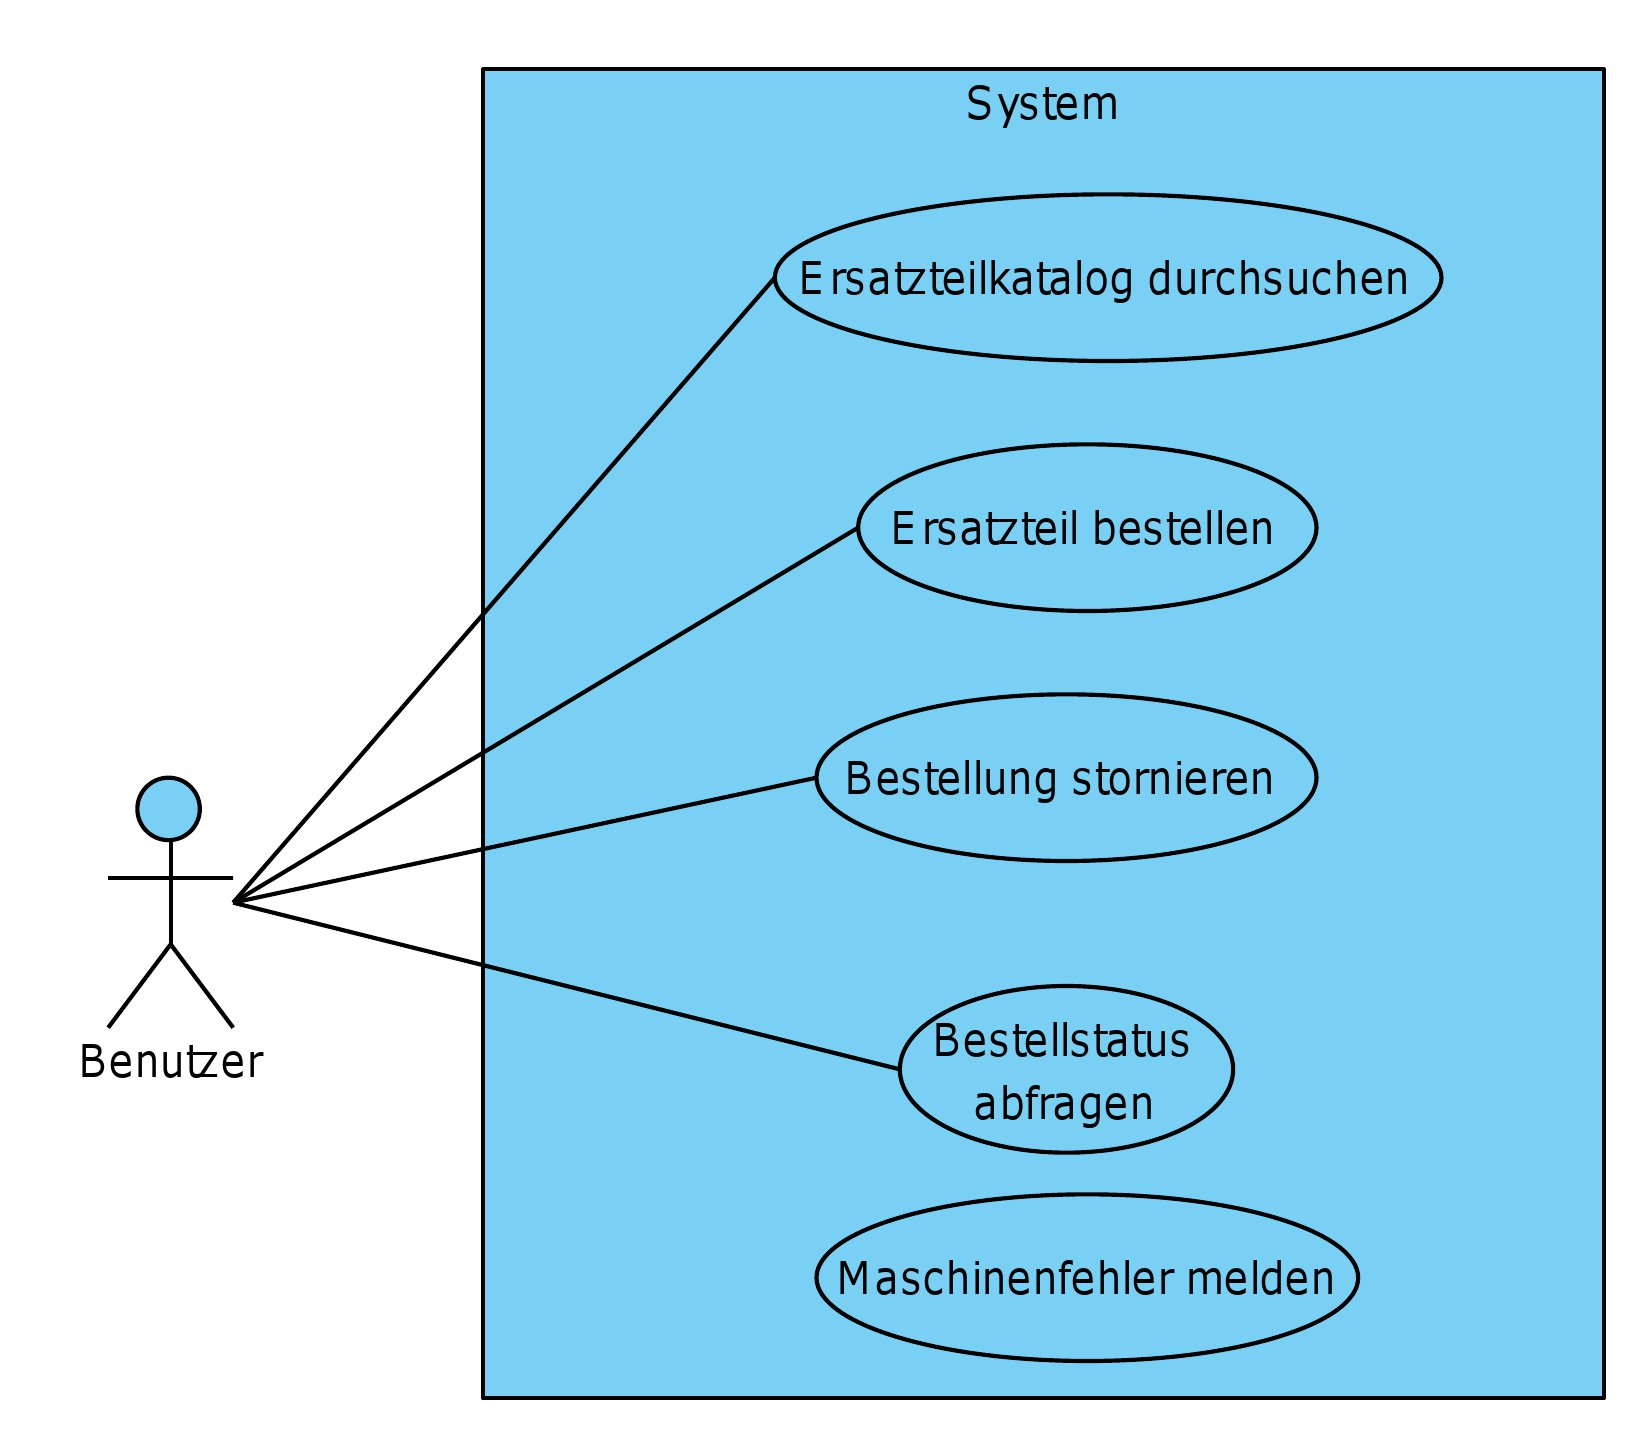
\includegraphics[width=1\textwidth]{Ersatzteilkatalog_use_case}
		      \caption{Gesch�ftsanwendungsf�lle Use-Case-Diagramm}
		      \label{fig:usecase}
		\end{figure}
      	
      	Nach der Kurzbeschreibung des Anwendungsfalls folgt als n�chstes die
      	Dokumentierung der Einzelheiten. Zuerst folgt eine textuelle
      	Beschreibung, die als Grundlage zur Erstellung des CIM dient. 
      	
      	Der Prototyp ``Spare Parts Catalogue'' soll folgende Funktionen
      	unterst�tzen:
      	
      	\begin{itemize}
            \item Ersatzteilkatalog durchsuchen
            \item Ersatzteil bestellen
            \item Bestellung stornieren
            \item Bestellstatus abfragen
            \item Maschinenfehler melden
          \end{itemize}
      	

      	\subsection{Erstellen eines Computation Independent Models}

		Die Funktionen von YASA lassen sich im Detail wie folgt beschreiben:
		%\begin{minipage}[!t]{0.4\textwidth}
		%\begin{table}[b]
	        	%\centering \leavevmode %Tabelle zentrieren
		        %\caption{}
		        %\label{tab:cross-platform}
		        %\addtocounter{footnote}{+1}
		        \newcolumntype{A}{%
				>{\columncolor{hellgrau}}p}
				\newcolumntype{B}{%
				>{\columncolor{hellgrau}}p}
				%\color{black}
				\arrayrulecolor{white}
				%TODO: \arrayrulewidth{3pt} irgendwie klappt das nicht... !
		        \begin{longtable}{||A{5cm}||B{10cm}||}
                %\centering \leavevmode
                %\hhline{|t:==:t|}
                \hline \hline
                \rowcolor{dunkelgrau}
                Funktion	 		&	Ersatzteilkatalog durchsuchen\\
                \hline \hline
                Kurzbeschreibung 	&	Ein Kunde m�chte den Ersatzteilkatalog
                						durchbl�ttern bzw. durchsuchen\\
                \hline \hline
                Akteur 				&	Benutzer\\
                \hline \hline
                Vorbedingungen		&	Kundendaten bekannt\\
                \hline \hline
				Teilhandlungen		&	Suchbegriff eingeben\\
                                    &   Ersatzteile bl�ttern\\
                                    &   Ersatzteil ausw�hlen (Detail
                                             ansehen)\\
                \hline \hline
				Nachbedingungen		&	-\\
				%\hhline{|t:==:t|}
				\hline \hline
				%\end{tabular}
				
				%\newline

		        %\begin{tabular}{||A{5cm}||B{10cm}||}
                \hline \hline
                \rowcolor{dunkelgrau}
                Funktion	 		&	Ersatzteil bestellen\\
                \hline \hline
                Kurzbeschreibung 	&	Ein Kunde m�chte ein Ersatzteil bestellen,
                						dessen Bezeichnung und Funktion ihm bereits 
                						bekannt ist\\ 
                \hline \hline 
                Akteur 				&	Benutzer\\
                \hline \hline
                Vorbedingungen		&	Ersatzteilkatalog
                						durchsuchen/ Maschinenfehler melden\\ 
                \hline \hline
				Teilhandlungen		&	Bestellvorgang einleiten\\
									&	Bestelldetails anzeigen\\
                                    &   Bestellung abschicken\\
                \hline \hline
				Nachbedingungen		&	Bestellung wurde erfolgreich �bermittelt\\
				\hline \hline
				%\end{tabular}

		        %\begin{tabular}{||A{5cm}||B{10cm}||}
                \hline \hline
                \rowcolor{dunkelgrau}
                Funktion	 		&	Bestellung stornieren\\
                \hline \hline
                Kurzbeschreibung 	&	Ein Kunde m�chte eine bereits ausgef�hrte
                						Bestellung stornieren\\ 
                \hline \hline 
                Akteur 				&	Benutzer\\ 
                \hline \hline
                Vorbedingungen		&	Ersatzteil wurde bestellt\\ 
                \hline \hline
				Teilhandlungen		&	Bestelldetails anzeigen\\
                                    &   Bestellung stornieren\\
                \hline \hline
				Nachbedingung bei Erfolg		&	Bestellung wurde erfolgreich storniert\\
				\hline \hline
				Nachbedingung bei Misserfolg	&	Bestellung konnte nicht storniert werden
													(evtl. wurde Bestellung schon versandt) \\
				\hline \hline
				%\end{tabular}

		        %\begin{tabular}{||A{5cm}||B{10cm}||}
                \hline \hline
                \rowcolor{dunkelgrau}
                Funktion	 		&	Bestellstatus abfragen\\
                \hline \hline
                Kurzbeschreibung 	&	Ein Kunde m�chte den Status seiner
                Bestellung abfragen 
                						(in Bearbeitung, versandt, nicht lieferbar, etc.)\\ 
                \hline \hline 
                Akteur 				&	Benutzer\\
                \hline \hline
                Vorbedingungen		&	Ersatzteil wurde bestellt\\ 
                \hline \hline
				Teilhandlungen		&	Bestelldetails anzeigen\\
									&	Bestellstatus anzeigen\\
                \hline \hline
				Nachbedingungen		&	-\\
				\hline \hline
				%\end{tabular}

		        %\begin{tabular}{||A{5cm}||B{10cm}||}
                \hline \hline
                \rowcolor{dunkelgrau}
                Funktion	 		&	Maschinenfehler melden\\
                \hline \hline
                Kurzbeschreibung 	&	Die Fertigungsmaschine hat einen Fehler
                festgestellt 
                					 	und kann nicht fortfahren. Eine Systemanalyse
                stellt fest, 
                						dass ein Teil der Maschine kaputt ist und sendet
                dem Benutzer eine Fehlermeldung \\ 
                \hline \hline 
                Akteur 				&   System\\ 
                \hline \hline
                Vorbedingungen 		&	Fehler im System\\
                				 	&	Fehler kann ermittelt werden\\
                \hline \hline
				Teilhandlungen		&	Systemmeldung mit Fehler erstellen\\
									&	passendes Ersatzteil ermitteln\\
									&	Systemmeldung an Benutzer senden\\
                \hline \hline
				Nachbedingungen		&	Nutzer wurde �ber Systemfehler informiert und kann
										Ersatzteil bestellen\\ 
				\hline \hline
				\end{longtable}
		%\end{table}
		%\end{minipage}

		Als n�chstes werden nun diese textuellen Beschreibungen m�glichst genau in
		Diagramme umgewandelt. Zur Erfassung dieser auf grober Detailstufe wird als
		Darstellung das Aktivit�tsdiagramm verwendet.
		
		\begin{figure}[h]
		      \centering	% zentrieren
		      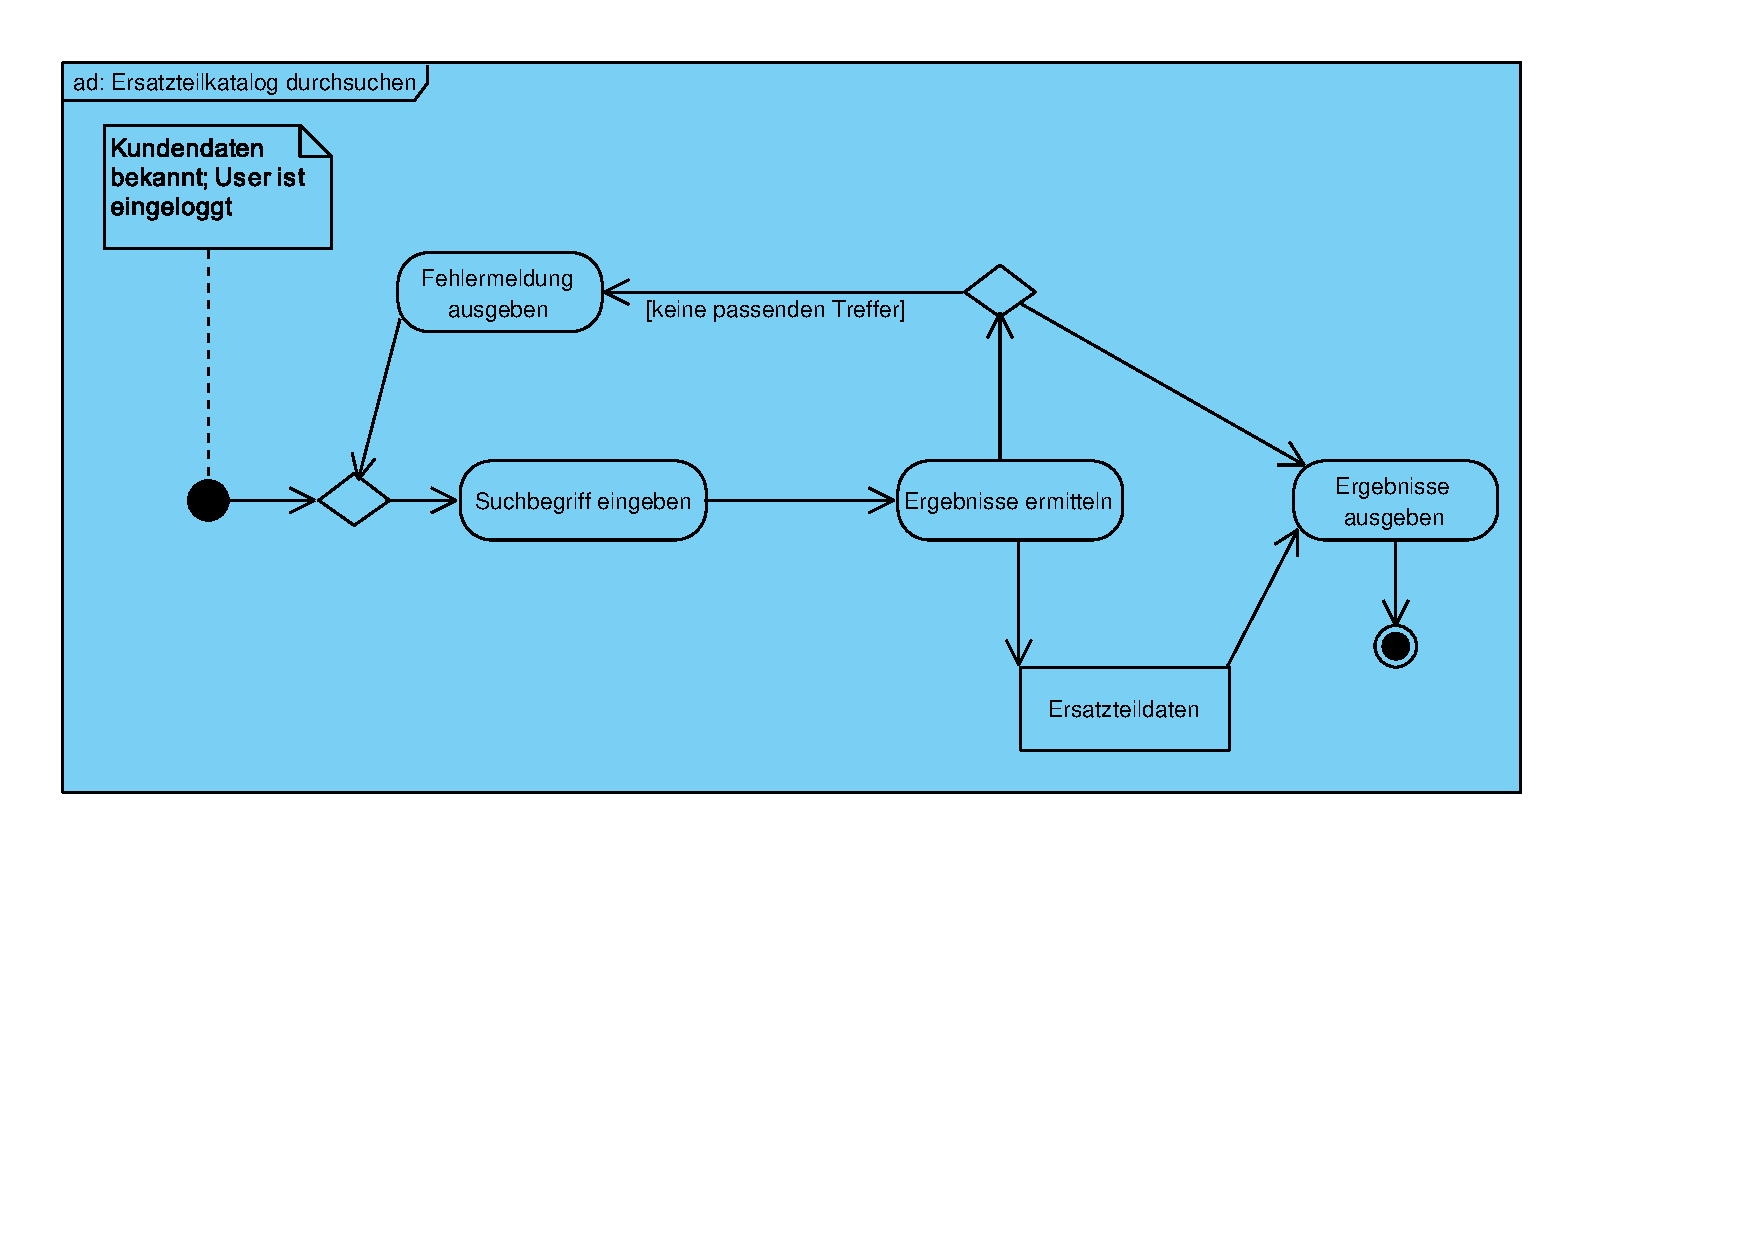
\includegraphics[width=1\textwidth]{activity_durchsuchen}
		      \caption{Aktivit�tsdiagramm Ersatzteilkatalog durchsuchen}
		      \label{fig:activity_durchsuchen}
		\end{figure}		

      	\subsection{PIM}
      	
      	Um die entworfenen Funktionen weiter umzusetzen und ein Platform
      	Independent Model zu generieren wird nun die Plattformunabh�ngige
      	Basisarchitektur festgelegt.
      	
      	Diese l�sst sich wie folgt darstellen:
      	
      	\begin{table}[h]
        	\centering \leavevmode %Tabelle zentrieren
        	\caption{Architektur von YASA-Anwendungen}
		    \label{tab:yasa-architecture}
% 	        \newcolumntype{A}{%
% 			>{\columncolor{hellgrau}}c}
 			\arrayrulecolor{black}
	      	\begin{tabular}{||c||}	          
	          \hline \hline  
	          	Pr�sentation / View \\
	          \hline  \hline
	          	Dialogfluss \\
	          \hline  \hline
	          	Gesch�ftslogik/Services \\
	          \hline  \hline
	          	Persistenz \\
	          \hline  \hline   	  
	        \end{tabular}
		\end{table}

		Als oberste Schicht im Diagramm \ref{tab:yasa-architecture} finden wir die
		Pr�sentationsschicht. Diese ist zust�ndig f�r die Darstellung des Inhalts auf
		dem jeweiligen Smartphone in einer f�r den Benutzer verst�ndliche Art und
		Weise. Darunter befindet sich der Dialogfluss. Hier werden Kontrollfl�sse der
		Anwendung definiert. Es folgt die Gesch�ftslogik des Systems, die in Form von
		Services zur Verf�gung gestellt werden. Sollen Daten im Rahmen der
		Gesch�ftslogik dauerhaft gespeichert und abrufbar sein, k�mmert sich die
		Persistenzschicht darum. 
		
		Die festgelegten Schichten k�nnen durch folgende UML-Profile modelliert
		werden:

		\begin{itemize}
          \item Pr�sentation (View): Metamodell zur Modellierung der auf dem
          Smartphone darzustellenden Oberfl�che in Form von Dialogmasken.
          Interaktionsm�glichkeiten des Nutzers mit der Oberfl�che und den
          enthaltenen Schaltfl�chen wird hier festgelegt.
          \item Dialogfluss (Pageflow Profile): Profil zur Modellierung von
          verzweigten Dialogfl�ssen
          \item Persistenz (Persistence Profile): Modellierung des persistenten
          Charakters von Entit�tsklassen
        \end{itemize}
        
        
        \subsubsection{Modellierung PIM}
        
        \begin{figure}[h]
		      \centering	% zentrieren
		      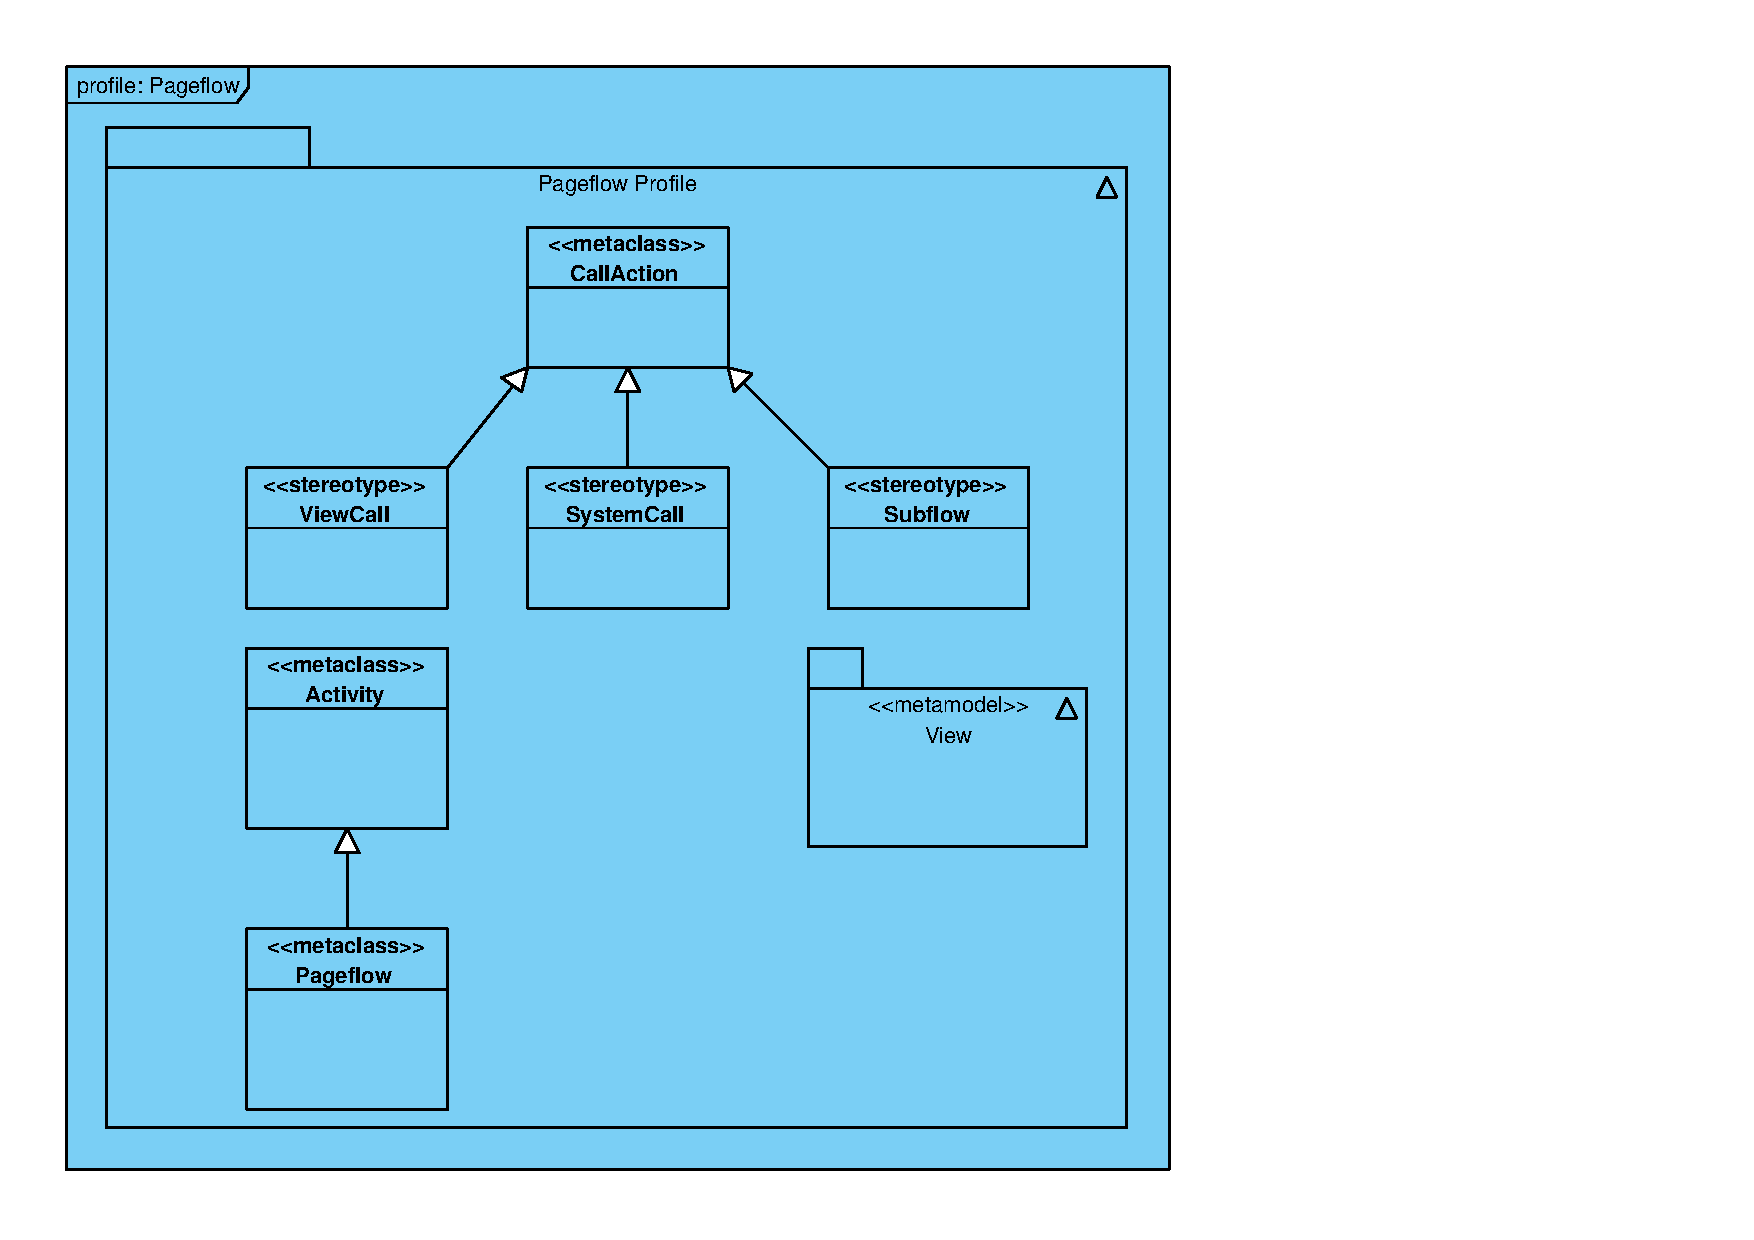
\includegraphics[width=1\textwidth]{profile_pageflow}
		      \caption{Definition von Pageflow Profile}
		      \label{fig:profile_pageflow}
		\end{figure}	

		\begin{figure}[h]
		      \centering	% zentrieren
		      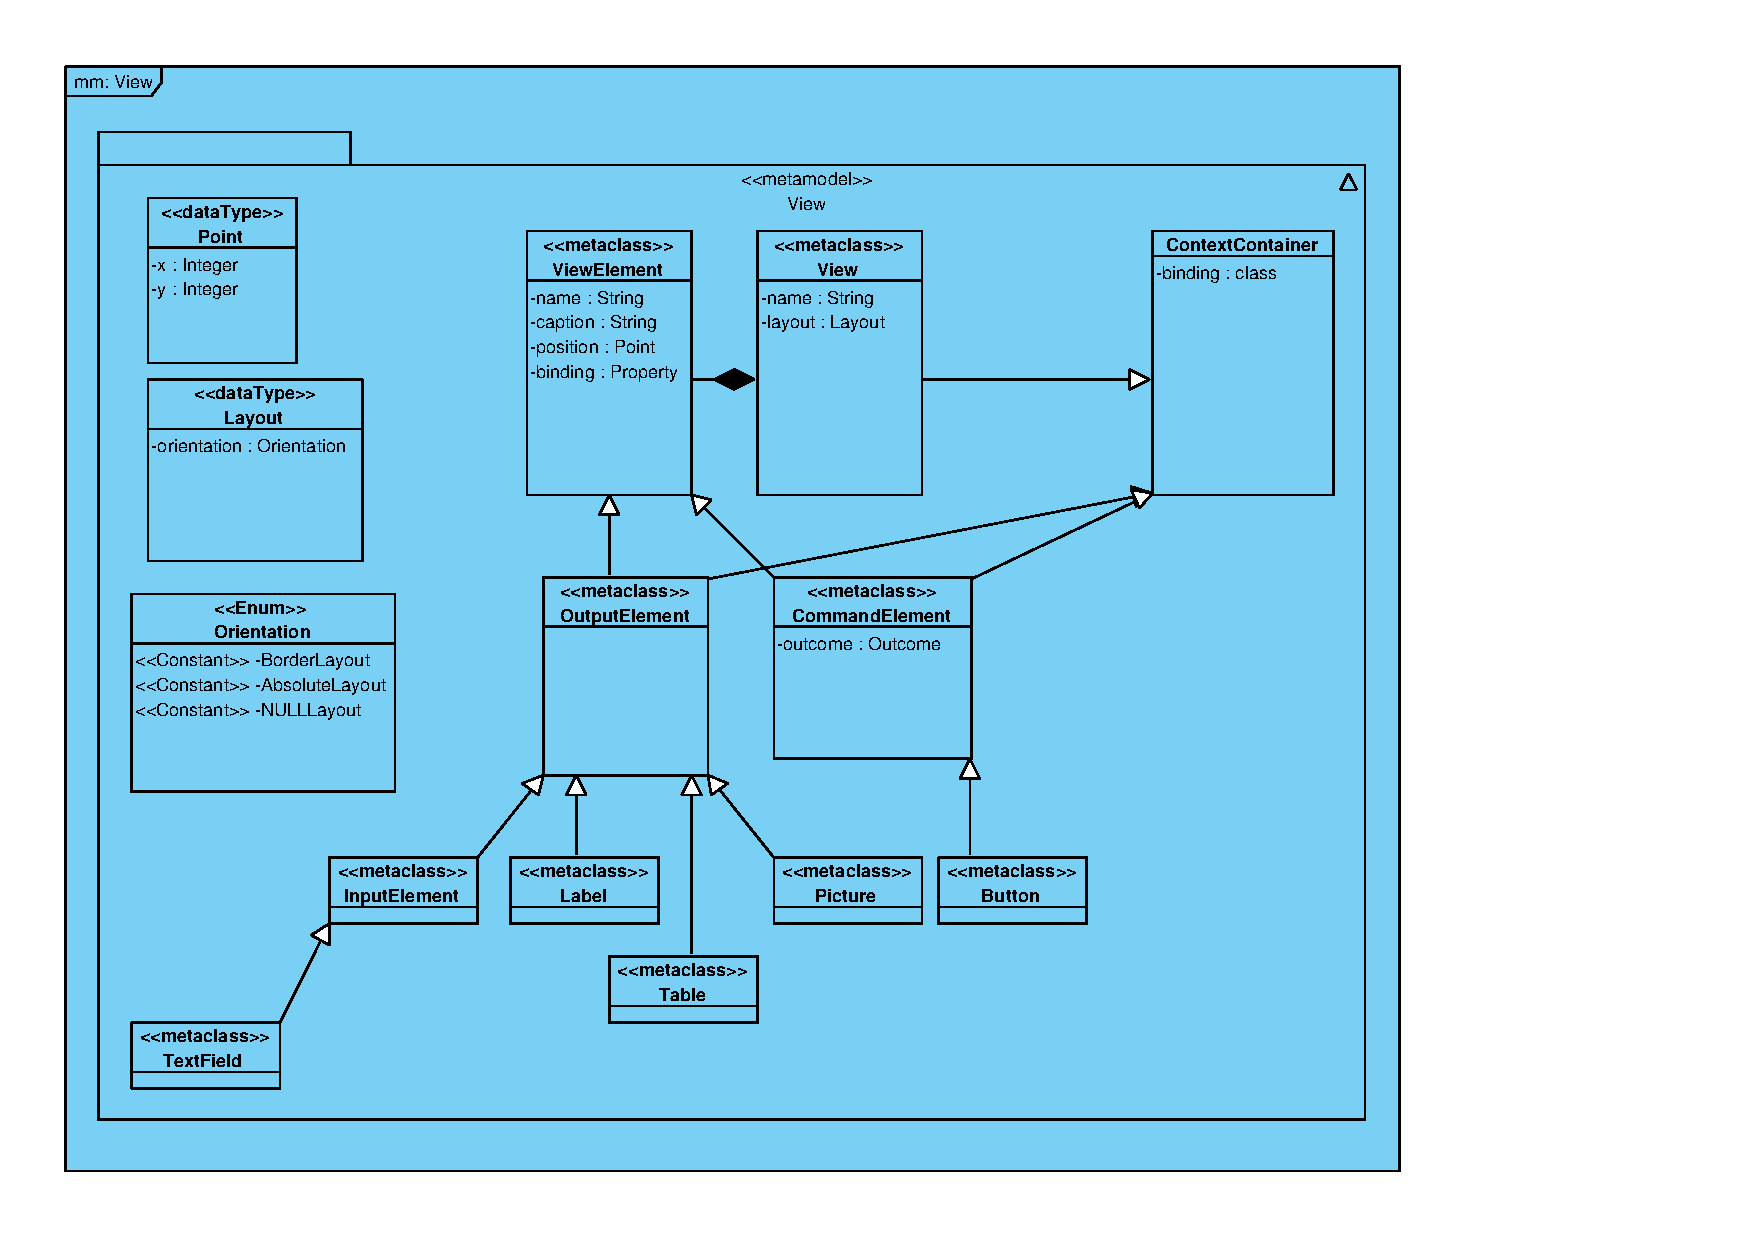
\includegraphics[width=1\textwidth]{profile_view}
		      \caption{Definition des Metamodells View}
		      \label{fig:profile_view}
		\end{figure}	
        
        Als Basisdiagramm soll uns das Aktivit�tsdiagramm dienen, welches durch
        weitere Elemente erweitert wurde. Zum einen w�re dies das Metamodell
        View, das die Konstrukte zur Modellierung der Dialogmasken enth�lt
        (siehe Abbildung \ref{fig:profile_pageflow}). Zum anderen...
        
        Als n�chstes zu definieren ist das View Metamodell. Hier wird festgelegt,
        welche Elemente zur Dartellung verwendet werden und wie der Benutzer die
        dargestellten Elemente manipulieren darf (Abbildung
        \ref{fig:profile_view}). Basiselement ist der \texttt{View}. Ihm werden
        beliebig viele View-Elemente zugeordnet. Weiterhin im Modell enthalten
        sind \texttt{OutputElemente} f�r die �bergebenden Modelldaten in
        grafischer Form und den \texttt{InputElementen}, die Werte des
        Pageflow-Kontextes durch Benutzereingaben aktualisieren. Daneben gibt es
        \texttt{CommandElemente}, an die ein \texttt{Outcome} geh�ngt werden
        kann(Kontrollflusssteuerung). Die Mitgeschickten Nutzdaten werden durch
        ein Element des Typs \texttt{ContextContainer} angehangen.
        
        
        Nach der Definition der verschiedenen Modelle lassen sich diese auf
        unsere Spezifikation anwenden. Im konkreten Fall ``Ersatzteilkatalog
        durchsuchen'' k�nnen wir den in Abbildung
        \ref{fig:ad_Ersatzteilkatalog_durchsuchen} dargestellten Dialogfluss
        generieren.
        
        \begin{figure}[h]
		      \centering	% zentrieren
		      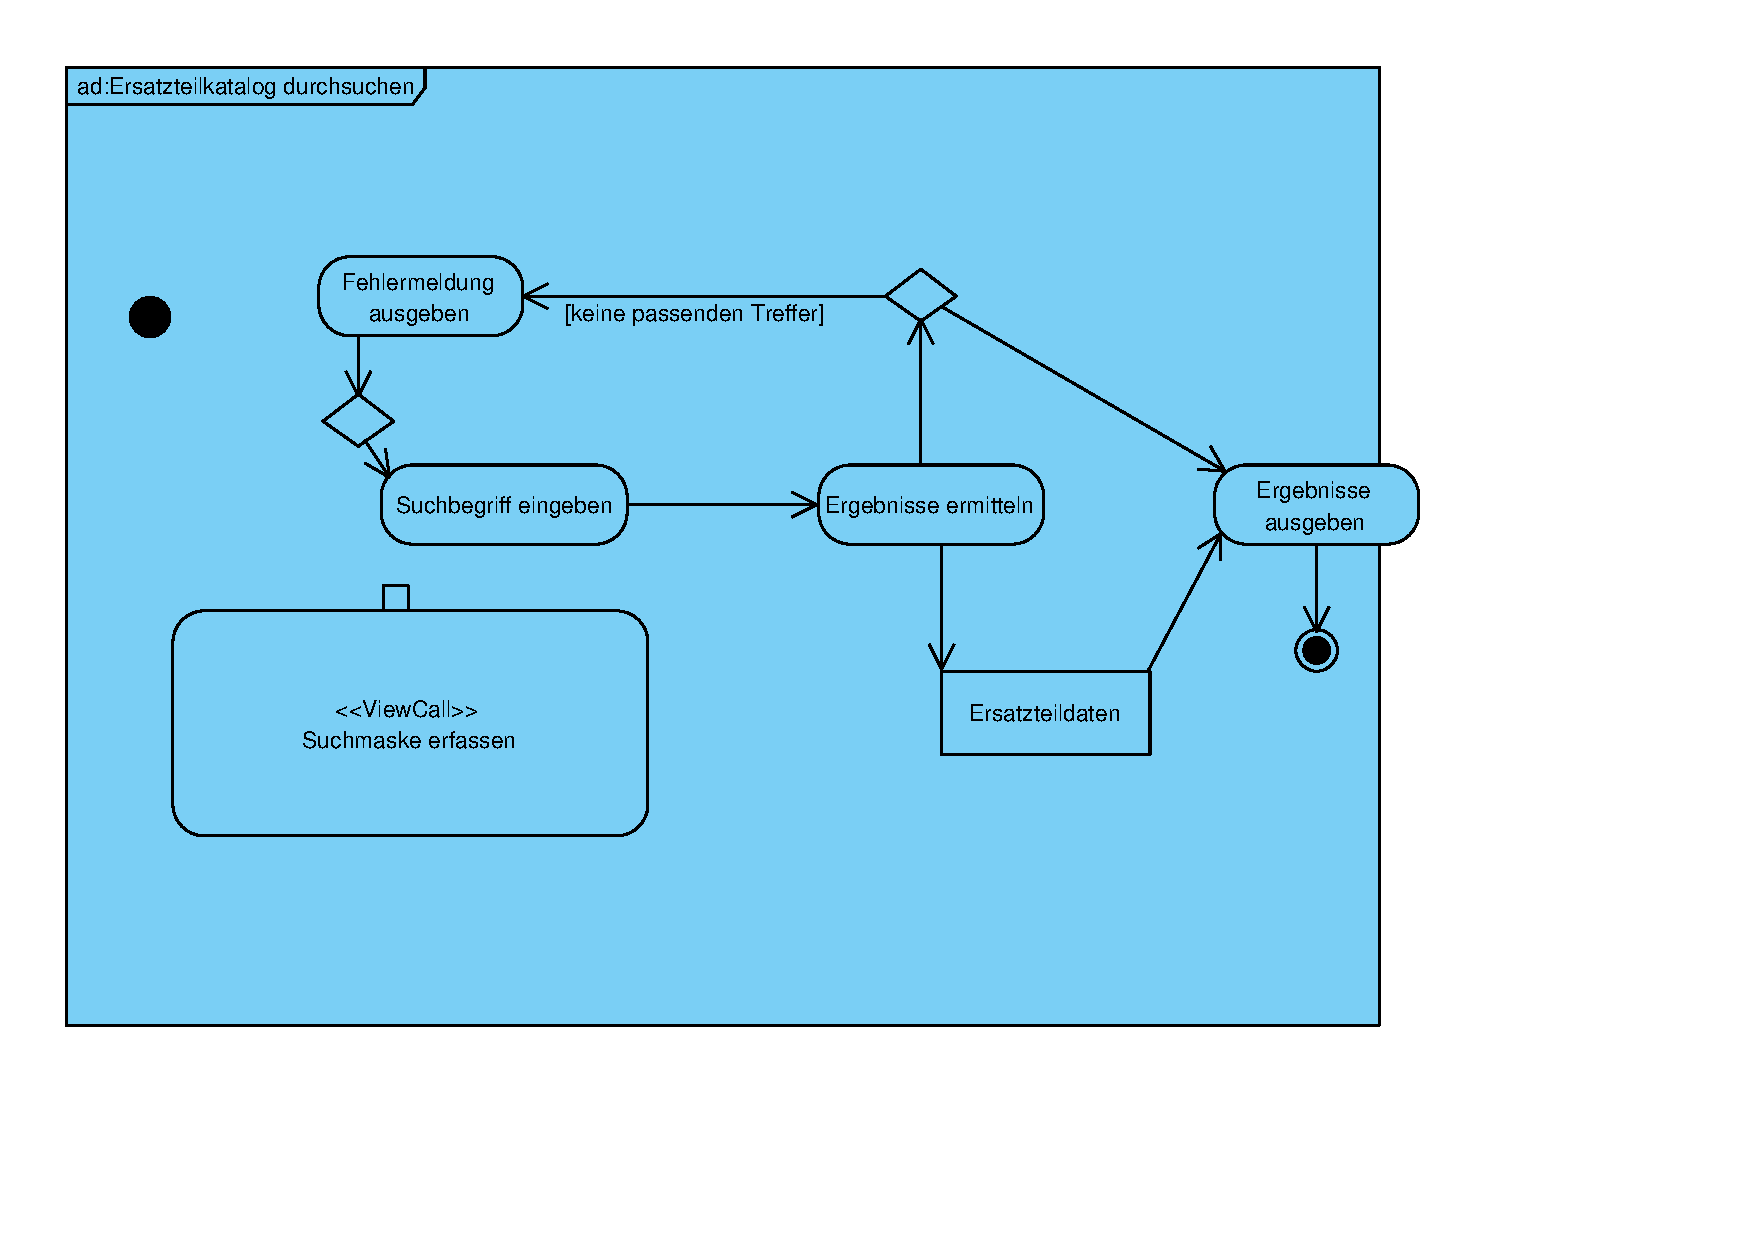
\includegraphics[width=1\textwidth]{ad_Ersatzteilkatalog_durchsuchen}
		      \caption{Dialogfluss ``Ersatzteilkatalog durchsuchen''}
		      \label{fig:ad_Ersatzteilkatalog_durchsuchen}
		\end{figure}	

		Bla fluss erkl�ren...
		
		%TODO: Skizze im Anhang einf�gen?
		Zur Beschreibung des Dialogflusses geh�ren ausserdem weitere Details, um die
		gestellten Anforderungen vollst�ndig abzubilden. (evtl. Verweis
		Entwurfsskizze). So muss jeder von einem \texttt{ViewCall} aufgerufene
		\texttt{View} weiter detailliert und mit dem entsprechenden Datenmodell
		verbunden werden (Abbildung \ref{fig:view_Ersatzteilkatalog_durchsuchen}).
        
        
        \begin{figure}[h]
		      \centering	% zentrieren
		      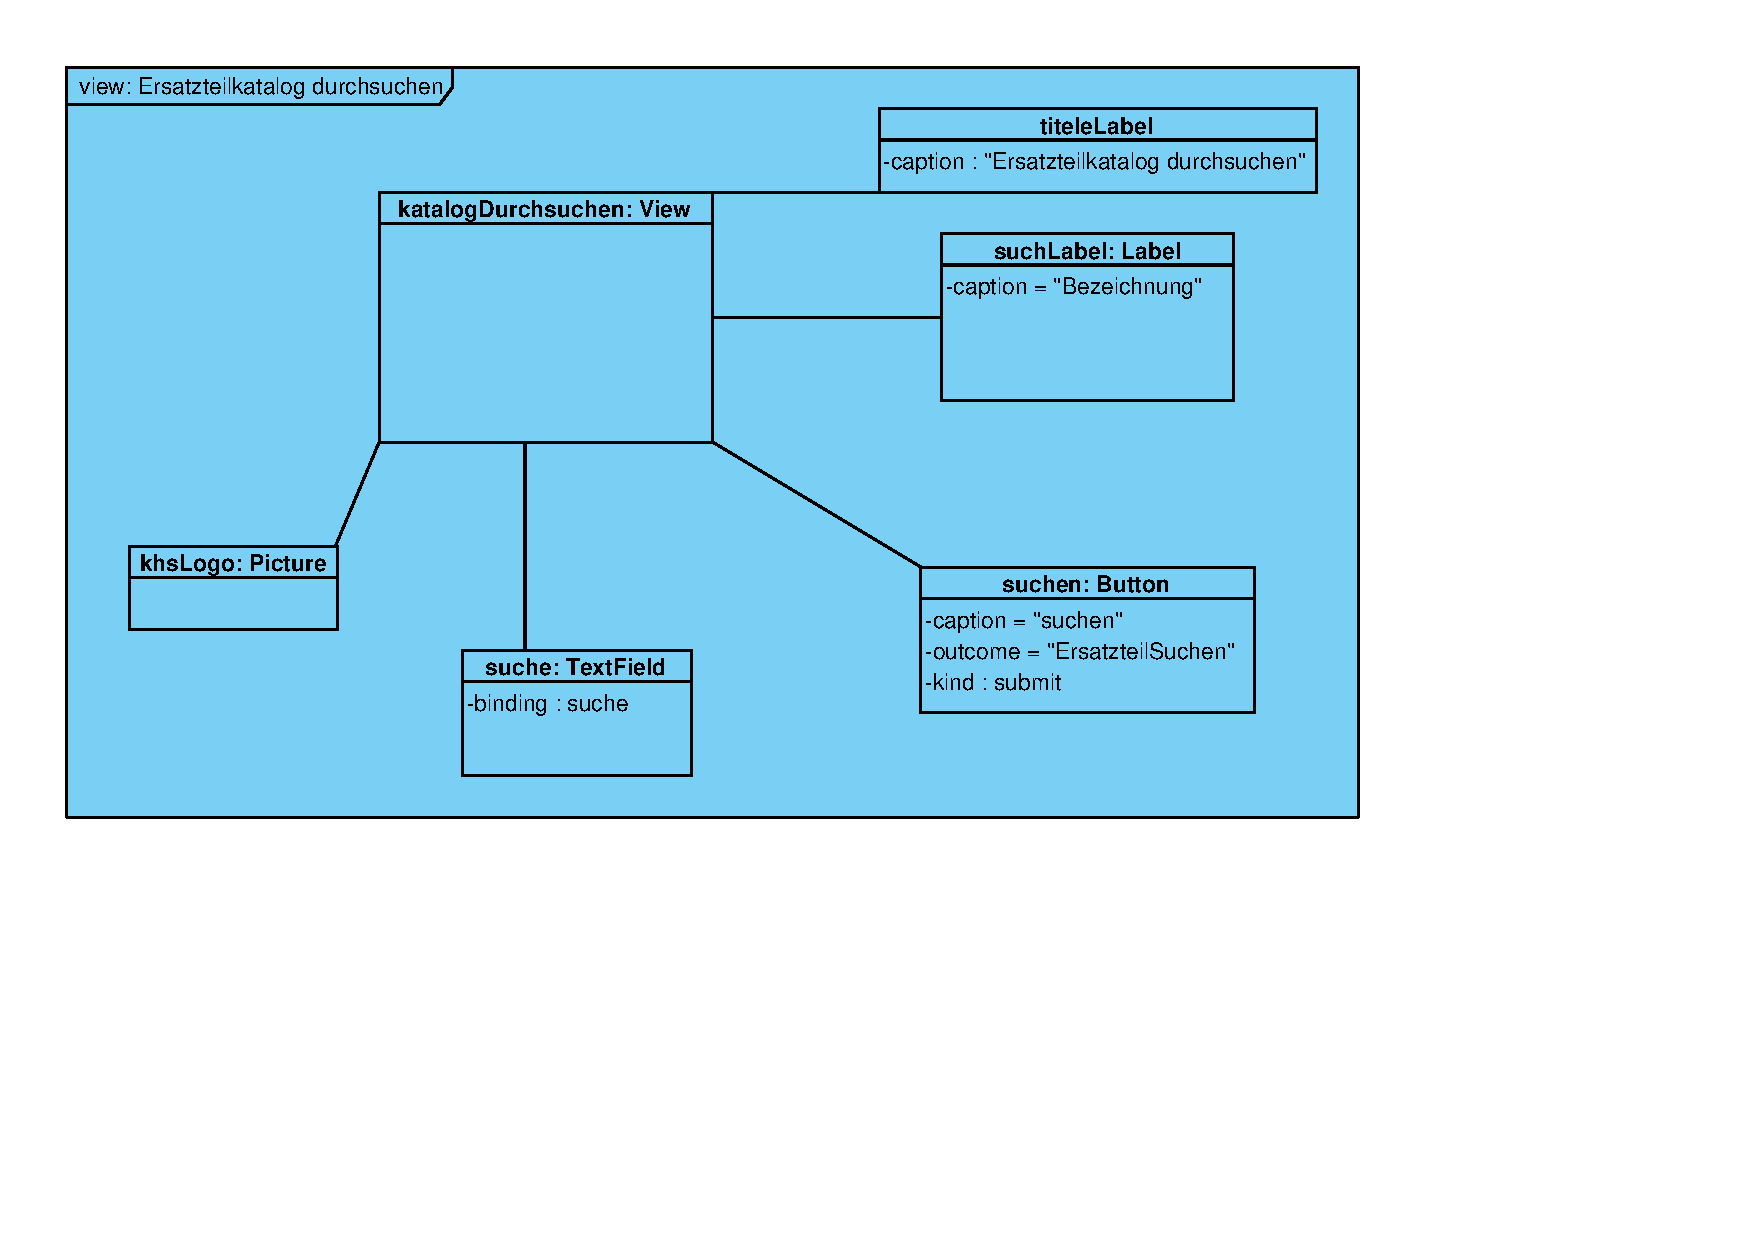
\includegraphics[width=1\textwidth]{view_Ersatzteilkatalog_durchsuchen}
		      \caption{Anwendung des View-Metamodells}
		      \label{fig:view_Ersatzteilkatalog_durchsuchen}
		\end{figure}	

      %TODO: Klassendiagramm erstellen f�r Persistenz. Aber was/wie?    
      
      \subsection{Vorhandene Modellierungs-/Transformationstools auf dem
      Markt}
          
          
      
      Verzichtet werden soll auf die Verwendung kommerziell-, propriet�rer
      Software zugunsten offener Standard und frei verf�gbarer
      Open-Source Technologien. Dabei sind auch �berlegungen zu den
      unterschiedlichen Lizenzen anzustellen.
      
      
%           \begin{itemize}
%             \item Die Transformationen erzeugen dabei aus den Elementen des
%             Quellmodells die Elemente des Zielmodells. �blicherweise laufen
%             die Transformationen von der abstrakteren zur konkreteren Schicht
%             (CIM -> PIM -> PSM -> Code)
%             \item Ist hier wirklich eine komplette Transformation n�tig? Dann
%             m�ssen mit OAW komplett alle Cartridges erstellt werden
%             \item Ansonsten Acceleo f�r Model-zu-Code Transformation; Daf�r
%             muss nur 1 Template je umzusetzendes Betriebssystem geschrieben
%             werden und die Templates k�nnen aus vorhandenem Beispielcode
%             generiert werden (sehr schnelle Erstellung von Templates m�glich)
%             %\item Evtl. AndroMDA (wird allerdings seit 2006 nicht mehr
%             %weiterentwickelt...)
%           \end{itemize}
      
      
      \subsubsection{OAW}
      \subsubsection{Acceleo}
      \subsection{Wahl der zu benutzenden Tools}
      
      Visual Paradigm
      
      

\chapter{Sicherheit in mobilen Netzen}
            
            \section{Sicherheitsprobleme in mobilen LANs und WANs}
            \begin{quote}
            ``Funknetze haben im Gegensatz zu leitungsgebunen Netzen
            zus�tzliche Gef�hrdungspunkte, die zumeist aus den verwendeten
            �bertragungsprotokollen und der nur begrenzt kontrollierbaren
            Ausbreitung der Funkwellen ergeben.'' [Eren06], S. 259
            \end{quote}

			\subsection{Bluetooth}
			
			Bluetooth erm�glicht die drahtlose Daten�bertragung und l�sst sich dabei
			leichter konfigurieren als Beispielsweise WLAN. Es wird dabei kein direkter
			Sichtkontakt zwischen den beteiligen Ger�ten ben�tigt (vgl. IRDA).
			
			%\subsubsection{Designschw�chen und Implementierungsschw�chen}
			
			In der Spezifikation von Bluetooth wird kein Verschl�sselungsalgorithmus
			vorgeschrieben, deswegen ist in der Standardkonfiguration vieler Hersteller
			die Verschl�sselung ausgeschaltet. Aber auch wenn diese aktiviert sein
			sollte, heisst dies nicht unbedingt, dass die Verbindung sicher ist.
			Der Verschl�sselungsalgorithmus bei Bluetooth baut auf einer XOR-Verkn�pfung
			von Klartext und Schl�sselstrom auf. Ein Angreifer kann Teile der
			versendeten Nachricht herausfinden, weil der zur Kommunikation benutzte
			TCP/IP-Header eine bekannte Form hat (hinsichtlich Gr��e und Aufbau).
			Als Folge sinken m�gliche Schl�sselkombinationen (Reduktion der
			effektiven Schl�ssell�nge von 128 Bit auf 84 Bit wegen des bekannten
			Headers). ``Brute-Force''-Angriffe werden somit erleichtert.
			
			Ein anderer Ansatzpunkt f�r Angreifer stellt der Zufallszahlengenerator dar.
			Zufallszahlen werden in einigen Sicherheitsfunktionen verwendet. In der
			Spezifikation des Bluetooth-Standards werden keine expliziten Anforderungen
			an diesen gestellt. Da verschiedene Hersteller wirtschaftlich g�nstige
			Algorithmen w�hlen, k�nnen teilweise durch die Bekanntheit dieser
			Algorithmen die Ergebnisse vorhergesagt werden.
			
			Der bei einer Authentifizierung notwendige vierstellige Pin-Code stellt auch
			bei einer 128-Bit Verschl�sselung leider immer noch keine ausreichende
			Sicherheit zur Verf�gung. Im Auslieferungszustand des Ger�ts ist
			dieser meist auf ``0000'' gesetzt. Wenn der Pin-Code vom Angreifer also
			richtig ermittelt werden kann, hat er die M�glichkeit die Kommunikation von
			gepairten Ger�ten ungest�rt zu belauschen.
			
			Alle Sicherheitsdienste bei Bluetooth sind in der Daten�bertragungsschicht
			(Schicht 2 des ISO-OSI-Schichtenmodells) angesiedelt. Somit gibt es keine
			Ende-zu-Ende Sicherheit. Die Verbindung wird zwar verschl�sselt, aber es
			fehlt eine nahtlose und durchgehende Datenverschl�sselung zwischen den
			Endger�ten.
			
			Das OBEX-Protokoll wird vor allem bei Bluetooth-Push-Diensten
			eingesetzt. Auch dieses hat Schw�chen. Der Stack wird vom
			Zulieferer und nicht vom Hersteller implementiert. Somit kann es passieren,
			dass Bluetooh-Ger�te, die den gleichen Stack und das gleiche virtuelle
			Dateisystem besitzen unauthorisierte Zugriffe aufs Filesystem (z.B.
			Telefonbuch) unbeabsichtigt offen legen.
			
% 			Spoofing. Vort�uschen falscher Identit�t. Ger�t A kommuniziert mit B. Ger�t
% 			C mit A und B. B nimmt Identit�t (Link Key) von C an und t�uscht diesen bei
% 			A vor. Kommunikation belauschen? Seite 270...
			
% 			Bluesniping mit Richtantenne. Bluetooth-Ger�te m�ssen normalerweise in
% 			unmittelbarer Reichweite sein (ca. 10 Meter entfernt). Mittels der
% 			Richtantenne lassen sich auch weit entfernte Ger�te  angreifen (bis zu 1
% 			Kilometer).
					
			\subsection{GSM}
						
			GSM wurde auf Basis der bereits bestehenden Festnetztechnik entwickelt. Die
			Verschl�sselung der Daten wurde nur als Option definiert, da in einigen
			L�ndern eine Verschl�sselung von staatlicher Seite untersagt ist. Auch wird
			auf den meisten Endger�ten nicht angezeigt, ob eine Verbindung verschl�sselt
			ist oder nicht. Ein weiterer Schwachpunt stellt der Umstand dar, dass Daten
			nur zwischen der BTS und dem Teilnehmer verschl�sselt werden. Das abh�ren
			von diesen Verbindungen ist an den diversen Schnittstellen der BTS zu
			anderen Netzkomponenten ohne gro�en Aufwand m�glich. Der potentielle
			Angreifer verschafft sich physischen Zugang zu einem BTS und kann von dort
			die Kommunikation belauschen bzw. manipulieren.
			
			Ebenfalls eine Schwachstelle ist der Kurznachrichtendienst SMS. Hier werden
			Nachrichten unverschl�sselt �ber den Signalisierungskanal �bertragen. Anhand
			der �bertragungsfrequenz kann so ein Angreifer Nachrichten mitlesen.
			
			\subsection{GPRS}
			
			GPRS stellt eine Erweiterung des GSM-Netzes um paketorientierte
			Daten�bertragung dar. Der Einstieg �ber das GPRS-Netz ins Internet wird als
			$G_{i}$-Schnittstelle bezeichnet. W�hrend der Datenkommunikation �ber GPRS
			ist der Teilnehmer anf�llig f�r im Netz verbreitete Gefahren und Angriffe.
			Falls der Datenverkehr unverschl�sselt stattfindet besteht die Gefahr, dass
			Daten durch einen Angreifer abgefangen und missbraucht werden. H�ufig
			rechnen Mobilfunkbetreiber mit solchen Gefahren und platzieren eine Firewall
			an der $G_{i}$-Schnittstelle.
			
			\subsection{UMTS}
			
			UMTS stellt eine Erweiterung auf Basis der verbreiteten Technik dar. Damit
			gew�hrleistet ist die Abw�rtskompatibilit�t zu GPRS/GSM. Prizipiell ist diese
			Technologie anf�llig f�r Denial-of-Service- und Impersonationsattacken. Unter
			Impersationsattacken versteht man die Verwendung eines kompromittierten
			Authentisierungsvektors, um sich unter der Identit�t des wahren Teilnehmers
			an das Netz anzumelden.
			
			%TODO: hier weiterschreiben!!!
			
			\subsection{HSDPA}
			
			fehlende info... buch zu alt. evtl. auf quelle im internet verweisen.
			
			\subsection{LTE}
			Neue Technik!!! noch nicht in Deutschland verf�gbar...
			
			\subsection{Wireless LAN}
			
			Die Mit der technischen Spezifikation verbundene Systemoffenheit
			zuverl�ssige und bequeme Einstiegspunkte ins ein Netzwerk zur Verf�gung zu
			stellen enbl��t leider auch abgeschottete private Netzwerke. Im Folgenden
			werden die verschiedenen Methoden der Verschl�sselung f�r Wireless LAN (kurz
			WLAN) erl�utert und konkret auf deren Schwachstellen eingegangen.
			
			\subsubsection{WEP}
			
			Das WEP-Protokoll verwendet zur Absicherung der Verbindung den symmetrischen
			Algoritmus RC4. 
			
			\begin{quote}
           	``Dieser ist ein Stromverschl�sselungsalgorithmus, der den
			Klartext �ber eine XOR-Operation mit einer Folge von Pseudozufallszahlen
			verkn�pft.'' [Eren06], S. 287
			\end{quote}
			
			Der WEP-Key wird entweder mit 40 Bit (WEP 64) oder 104 Bit (WEP 128) erzeugt.
			
			%\subsubsubsection{Schw�chen von WEP}
			
			%Schw�chen von WEP
			
			Schlechte Implementierungen des Initialisierungsvektors (der zusammen mit
			dem WEP-Key dazu benutzt wird die �bertragung zu verschl�sseln) f�hren zu
			Kollisionen in den �bertragenen Daten. Angreifer k�nnen diese Kollisionen
			erkennen und dadurch auf die unverschl�sselte Nachricht schliessen.
			
			Bei WEP fehlt eine gegenseitige Authentisierung. Aufgrund der Einfachheit,
			eine Netzwerkkomponente (insbesondere MAC-Adresse) zu f�lschen entsteht
			damit eine wesentliche Sicherheitsl�cke.
			
			Nach RFC 1024 m�ssen alle IP- und ARP-Pakete stest mit einem ``0xAA'' beginnen.
			Dies kann von einem Angreifer ausgenutzt werden, um den WEP-Schl�ssel zu
			ermitteln. Mit relativ wenig Aufwand wird genug Chiffretext gesammelt. Um
			den Schl�ssel ermitteln zu k�nnen, m�ssen die ersten Bystes des Klartextes
			bekannt sein. Aufgrund der Anforderung nach RFC haben Angreifer also
			leichtes Spiel.
			
			
			
			\subsubsection{WPA}
			
			Der grundlegende Unterschied zu WEP ist die Verwendung von TKIP als
			Verschl�sselungsprotokoll. Prinzipiell l�sst sich WEP mittels Software- und
			Firmware-Updates auf WPA upgraden.
			
			Um die Schwachstellen von WEP auszumerzen implementiert WPA dynamische
			Schl�ssel f�r jedes versendete Paket. Dabei besitzt jeder Benutzer einen
			eigenen Schl�ssel.
			
			WPA ist anf�llig f�r W�rterbuchattacken, da der Preshared Master Key direkt
			aus der Passphrase und der SSID abgeleitet wird. F�r einen solchen Angriff
			reicht ein aufgezeichneter TKIP-Handshake aus. Allerdings ben�tigen die
			anschlie�enden Berechnungen einen aktuellen High-End-PC, da gerade einmal
			ca. 70 Passw�rter pro Sekunde gepr�ft werden k�nnen. Falls also ein
			geeignetes starkes Passwort gew�hlt wurde geht von dieser Attacke eine nur minimale
			Gefahr aus.
			
			\subsubsection{WPA2}
			
			Da der bei WEP und WPA zugrundeliegende Algorithmus RC4 als gebrochen gilt,
			wurde bei WPA2 die AES Verschl�sselung eingesetzt. Dabei bleibt WPA2 noch zu
			WPA abw�rtskompatibel.
			
			Eine ``Brute-Froce''-Attacke ist zwar rein theoretisch denkbar, aber sehr
			unwahrscheinlich, da die Wahrscheinlichkeit f�r eine identische Pr�fsumme
			eines MAC bei ca. 1 : 1 Mio. liegt. Ausserdem wird bei einer Attacke ein 60
			Sekunden andauernder Blackout (Unterbrechen der Verbindung) des Access
			Points verwendet, um etwaige Attacken abzublocken. Allerdings kann eine
			``Denial-of-Service''-Attacke so durchaus erfolgreich sein, wenn es der
			Angreifer nicht auf den Schl�ssel abgesehen hat.
            
            \section{Denkbare Angriffsformen auf Mobiltelefone in einer
            Firmeninfrastruktur}
            
            \begin{itemize}
	            \item Aussp�hen von Daten: Der Angreifer verschafft sich
	            Zugang zu relevanten Daten, die auf dem jeweiligen Ger�t
	            gespeichert sind. Dazu geh�ren Kontaktlisten, E-Mails, SMS und
	            andere vertrauliche Dokumente und Dateien.
	            \item Nutzung eigener Dienste und Zug�nge: Wird eine
	            Authentifizierung lediglich beim Einschalten des Ger�ts verlangt,
	            kann das Ger�t im Verlustfall ganz leicht von Kriminellen wie ein
	            Schl�ssel f�r Dienste und Zug�nge genutzt werden. Dadurch k�nnen
	            Sicherheitsmechanismen, die Firmen-, Service- oder Datenstrukturen
	            vor unbefugtem Zugang sch�tzen, ausgehebelt werden.
	            \item Manipulation der Software-Komponenten: Dabei k�nnen Angriffe
	            auf Netzwerke in Verbindung mit der Synchronisation zwischen
	            mobilem Ger�t und dem Firmennetz erfolgen, um Informationen oder
	            Daten direkt zu erhalten. Dar�ber hinaus bietet die Konfiguration
	            von Proxies, die bei der Internetkommunikation genutzt werden, die
	            M�glichkeit des Abh�rens und Aufzeichnens, aber auch der
	            Manipulation (Tracing, Capturing, Logging) der an das Ger�t
	            zur�ckgesendeten Informationen.
	            \item �berwachung: Moderne Smartphones bieten neben
	            Kommunikationsschnittstellen wie GPRS, 3G, WLAN und Bluetooth
	            unl�ngst auch GPS-Module. Damit lassen sich raumbezogene
	            Referenzinformationen ablegen, die das Erstellen eines genauen
	            Bewegungsprofils erm�glichen. Dazu ist eine Manipulation des
	            Ger�ts notwendig, die aber keines Diebstahls bedarf.
            \end{itemize}
            
            \section{Sicherheitsmechanismen}
            
            Folgende Mechanismen sollen dazu beitragen, dass Firmenrelevante
            Daten nicht einfach von Dritten ausgesp�ht werden k�nnen.
            
            \subsection{WLAN sichern mit Radius}
            Beim WLAN-Einsatz in Unternehmen reicht die simple
            Authentifizierung �ber ein gemeinsames Passwort (Shared Secret)
            mit WPA-PSK nicht: Das Geheimnis ist bei gro�er Verbreitung zu
            schnell keines mehr. Sp�testens wenn ein Kunde vor�bergehend einen
            Zugang bekommen hat, muss man es �ndern. Mit serverseitig
            zugeteilten Passw�rtern erspart sich der Administrator viel Arbeit
            und Nachfragen seiner Nutzer.
            
            F�r solche Einsatzf�lle ist die Spielart WPA Enterprise gedacht,
            bei der die WLAN-Basisstation Verbindungsanfragen von ihren
            Clients �ber das Protokoll IEEE 802.1x mit einem nachgelagerten
            Radius-Server aushandelt. Auf Linux-Systemen ist dazu das
            Open-Source-Paket Freeradius g�ngig. [Radius10], letzter Abruf
            07.12.2010
            
            Mit dem Extensible Authentication
            Protocol (EAP) unterst�tzt es verschiedene kryptografisch
            gesicherte Methoden (EAP-TLS/-TTLS, PEAP, LEAP),
            One-Time-Passworte und SIMs. F�r die Authentifizierung sind
            Username/Passwort-Kombinationen oder Zertifikate gebr�uchlich.

			Damit Daten nicht im Klartext durch die Luft beziehungsweise �ber die
			Leitung zwischen Basisstation und Radius-Server laufen, verschl�sselt
			Freeradius diese. Voraussetzung daf�r ist, dass auf dem Client mindestens ein
			Stammzertifikat (Root CA Certificate) installiert ist, von dem das Zertifikat
			des Radius-Servers abgeleitet ist. Mit dem Stammzertifikat pr�ft der Client
			auch, dass er sich beim richtigen Radius-Server authentifiziert.
			
			\subsection{MDM}
			
			\begin{figure}
			  %\begin{minipage}[b]{0.48\textwidth}
			      \centering	% zentrieren
			      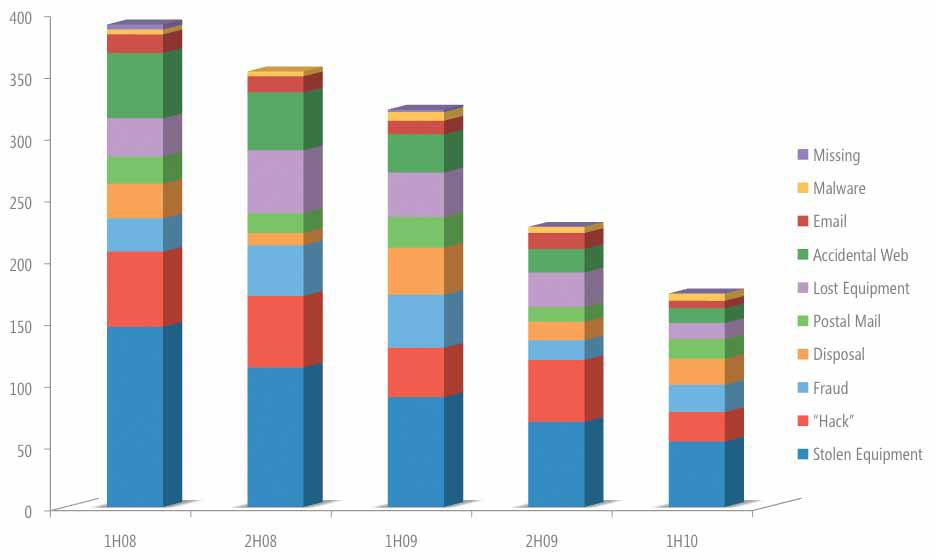
\includegraphics[width=0.8\textwidth]{microsoft_security_trends}
			      \caption{Datenverluste in Unternehmen}
			      \label{fig:microsoft_security_trends}
			\end{figure}
%TODO: Quelle
			
			
			Wie man der Abbildung \ref{fig:microsoft_security_trends} entnehmen kann
			f�hrt der Diebstahl von Endger�ten am h�ufigsten zu Sicherheitseinbr�chen in
			Systemen.
			
			MDM (Mobile Device Management) bezeichnet die M�glichkeit von der Ferne aus
			auf ein Mobiltelefon zuzugreifen und dieses gegebenenfalls zu sperren bzw.
			Daten zu l�schen oder andere Sicherheitsmechanismen auszul�sen.
			
			Die derzeitige Funktionspalette umfasst: 

			\begin{itemize}
              	\item auf dem Ger�t enthaltene Daten sichern und wieder
              	aufspielen (``Backup \& Restore'')
              	\item Software-Updates zentralisiert und drahtlos aufspielen, um
    			Sicherheitsl�cken schnell zu schlie�en (``Update Over The Air'')              
    			\item ein gestohlenes oder verlorenes Ger�t aus der Ferne sperren und
    			seine Daten l�schen (``Remote Lock \& Wipe'') sowie per GPS verfolgen
    			(``Mobile Tracking'')
    			\item einzelnen Nutzern differenzierte Rechte zuteilen - vom
    			Internet-Zugang bis zur Installation von Programmen (``Policy \&
    			Provisioning'')
    			\item  Statistiken erstellen, wie ein Smartphone genutzt wird und welche
    			Kosten anfallen (``Logging \& Accounting'')
            \end{itemize}

			Bei den MDM-L�sungen bekommen die Ger�te eine Identit�t zugewiesen, die mit den
			entsprechenden Zugangsberechtigungen und Funktionseinschr�nkungen verkn�pft ist.
			Im Idealfall bekommt der Nutzer f�r sein Smartphone nur noch ein Passwort, mit
			dem er sich einmalig f�r die Erstkonfiguration anmelden kann. W�hrend der
			normalen Nutzung im Alltag k�nnen die Firmen-Administratoren mittels MDM dann
			zentral Software-Updates verteilen, Ger�te sperren oder durch
			Konfigurations�nderungen schnell auf Sicherheitsl�cken reagieren. Wird das
			Smartphone schlie�lich ausgemustert oder verl�sst der Nutzer das Unternehmen,
			werden mittels MDM Berechtigungen gel�scht, Unternehmensdaten getilgt oder die
			Konfiguration auf ein neues Endger�t �bertragen.
									
			Der Markt f�r MDM-L�sungen ist derzeit noch �bersichtlich. Statistiken �ber
			Marktanteile existieren nicht. Zu den gro�en drei, die immer wieder genannt
			werden, geh�ren jedoch die US-Unternehmen Mobile Iron, Good Technology und
			Sybase. Ihre Produkte unterscheiden sich dabei vor allem im Detail - w�hrend
			Good Technology gro�es Know-how in Sales-Umgebungen verspricht, streicht man bei
			Mobile Iron die Handhabbarkeit unterschiedlicher Smartphone-Plattformen heraus.
			Sybase wirbt wiederum mit einer guten Anbindung an die hausinterne IT. Zumeist
			bezahlen Unternehmen einen Sockelbetrag plus eine Lizenzgeb�hr pro Nutzer. Mit
			insgesamt einigen Tausend Euro pro Jahr m�ssen die Firmen dabei rechnen.
			Anbieter wie Mobile Iron haben f�r Neukunden aber auch Lockofferten von nur vier
			Dollar pro Nutzer und Monat (plus Sockelbetrag) im Angebot.
									
			Was die Sache noch komplizierter macht: In vielen Firmen werden l�ngst nicht
			mehr nur reine Businessger�te wie die Blackberrys des kanadischen Anbieters RIM
			eingesetzt. Apples iPhone beispielsweise hat mittlerweile ebenfalls einen
			Siegeszug in Unternehmen angetreten. Der traditionsreiche IT-Dienstleister
			Unisys etwa, der f�r Firmen und Regierungen auf der ganzen Welt arbeitet,
			benutzt iPhones, um Server zu �berwachen, aber auch f�r h�chst
			sicherheitskritische Anwendungen wie die Steuerung von Systemen zur
			Kamera�berwachung.
									
			Ein weiterer kritischer Punkt sind private Anwendungen auf Firmen-Smartphones.
			Ger�te wie das iPhone laden geradezu dazu ein, neben gesch�ftlichen Apps auch
			Spiele zu installieren oder Multimedia-Content zu konsumieren. Schlie�en l�sst
			sich dieses Sicherheitsloch derzeit nur, indem Firmen das Aufspielen    privater
			Inhalte ganz verbieten.
			% TODO: �berarbeiten/umschreiben... evtl. streichen
            
            \section{Entscheidung f�r �bertragungstechnik}
            
            % evtl. bluetooth lt. gespr�ch?
            
          begr�ndung durch schlussvolgerung aus sicherheitsl�cken und
          erl�uterung sicherheitskonzept, damit die schwachstellen der technik
          nicht ausgenutzt oder nur zum teil ausgenutzt werden k�nnen.
           	
          \texttt{YASA} soll m�glichst unabh�ngig vom Standort genutzt werden
          k�nnen. Eine solche Flexibilit�t l�sst sofort einige der
          angesprochenen �bertragungstechniken ausscheiden. Die einzige
          M�glichkeit zu garantieren, dass die Applikation wirklich
          Standortunabh�ngig genutzt werden kann ist die Verwendung
          providerabh�ngigen Netzen. F�r WLAN, Bluetooth \& Co. muss das Ger�t
          immer in Reichweite mit der Empf�ngerstation bleiben, deswegen fallen
          diese weg.
          
          

           	
           	
           	
           	
           	
           	
           	
           	

           	


\chapter{Mobile Betriebssysteme und Entwicklungsvoraussetzungen}
		Der Smartphonemarkt ist relativ gro� und un�bersichtlich. Im Nachfolgenden
		werden verschiedene Betriebssysteme angesprochen und verglichen, um eine
		Ausgangsbasis zu schaffen. Dabei wird verst�rkt auf die derzeitigen
		Marktf�hrer eingegangen (vgl. Abbildung \ref{fig:SP-marktA}). %auf Seite
		%\pageref{fig:SP-marktA}). 
		
		Wie man der Grafik entnehmen kann sind dies vor Allem das von Nokia
		verbreitete Symbian, Google's Android und iOS von Apple. Symbian
		bleibt zwar laut Statistik wieterhin unangefochtener Marktf�hrer,
		befindet sich allerdings auf dem absteigenden Ast. Android und iOS
		bauen ihren Marktanteil immer weiter aus und werden Symbian so wohl
		bald vom Thron stossten. 
		
% 		Weiterhin werden zur Vollst�ndigkeit noch andere Betriebssysteme erw�hnt, die
% 		sich im Moment im Umlauf befinden. Allerdings ...
		
		%TODO Grafik: eventuell direkt als Tabelle neu basteln, damit die Grafik
		% nicht schlechte skaliert...
		\begin{figure}
		  %\begin{minipage}[b]{0.48\textwidth}
		      \centering	% zentrieren
		      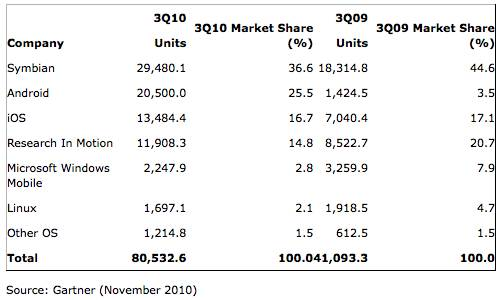
\includegraphics[width=0.8\textwidth]{MA_smartphones}
		      \caption{Smartphone - Marktanteile}
		      \label{fig:SP-marktA}
		  %\end{minipage}% Dies Prozent ist wichtig! (kein horiz. Abst. zw. minipages
		\end{figure}
		
		\section{iOS}
		\begin{itemize}
          \item Grundlagen und Bedienung
          %\item Voraussetzungen f�r die Entwicklung
          %\item -> speziell AppStore
          %\item Jailbreak ansprechen
          %\item Alternative Entwicklung ohne die MAC XCode Tools aufzeigen
          \item Hinweis auf Legalit�t/Schwierigkeit
        \end{itemize}
        
	        \subsection{Architektur}
	        Apple �berl�sst dem Entwickler beim iPhone nicht direkten Zugriff auf
	        die Hardware, sondern �ber diverse Layer (Tabelle
	        \ref{tab:iphonearch}), die zwischen Hardware und der Applikation vermitteln sollen. Diese Layer beschreiben das iOS. [Koller10]
	        
	        \begin{table}%[h]
	        	\centering \leavevmode %Tabelle zentrieren
		        \caption{Die Architektur des iPhone OS}
		        \label{tab:iphonearch}
		        %\addtocounter{footnote}{+1}
		        \begin{tabular}{||c||}
		        \hline
		        \hline
		        \texttt{Eigene (native) Anwendungen}\\
		        \hline
		        \hline
		        \texttt{Cocoa Touch}\\
		        NSFFoundation, UIKit\\
		        \hline
		        \hline
		        \texttt{Media}\\
		        (Quartz, Core Animation, Open GL, Core Audio, ...)\\
		        \hline
		        \hline
		        \texttt{Core Services}\\
		        (Core Location, Adress Book, SQLite, CFNetwork, ...)\\
		        \hline
		        \hline
		        \texttt{Core OS}\\
		        (I/O, Threads, Sockets, Bonjour, Key Chain, ...)\\
		        \hline
		        \hline
		        \end{tabular}
			\end{table}

	        \subsection{iOS Komponenten}
	        
	        Der ``Cocoa Touch Layer'' beinhaltet die am h�ufigsten von 
	        Entwicklern genutzten Frameworks zum Programmieren des iPhones. Er
	        basiert auf der Standard Mac OSX Cocoa API und wurde an die
	        Bed�rfnisse des iPhones angepasst. Die wichtigsten Komponenten hieraus
	        sind das ``UIKit Framework'' (Zust�ndig z.B. f�r das erstellen des
	        Userinterfaces), der ``Push Nocification Service'' (Nachrichten werden
	        eventgesteuert an den Benutzer weitergegeben), das ``Message UI
	        Framework'' und das ``Address Book UI Framework''.
	        
	        Eine Schicht unter Cocoa befindet sich der ``Media Layer''. Dieser ist
	        daf�r zust�ndig, dass das iPhone mit Audio-, Videodaten und
	        (3D-)Grafik umgehen kann.
	        
	        Mit dem ``Core Service Layer'' hat man beispielsweise die M�glichkeit
	        auf die im System integrierte mySQL Datenbank zuzugreifen. Weiterhin
	        l�sst sich zum Beispiel mit dem ``Data Framework'' das MVC Prinzip f�r
	        Applikationen umsetzen.
	        
	        Der ``Core OS Layer'' liegt direkt auf der Hardware auf. Hier werden
	        einige Dienste zur verf�gung gestellt, wie zum Beispiel der
	        Netzwerkzugriff (low level), der Zugriff auf externe Ger�te oder
	        Betriebssystemspezifische Dinge wie Speichermanagement oder wie mit
	        Threads umzugehen ist.       
	        
	        \subsection{Sicherheit}
	        
	        Entwickelt wird f�r das iPhone in Objective C. Der Quellcode wird in
	        Machinensprache �bersetzt und l�uft ohne zus�tzliche Laufzeitumgebung.
	        Apples Sicherheitskonzept sieht eine Isolierung der Apps und Prozesse
	        mittels einer Mandatory Access Control vor.
	        
	        In der Vergangenheit stellte sich immer wieder heraus, dass trotz
	        Sandboxing Apps zumindest lesend auf Konfigurationsdateien zugreifen
	        k�nnen. Das liegt unter Anderem auch an den Mac OS X �hnlichen
	        Zugriffsregeln auf Basis von Regular Espressions. Es werden
	        Zugriffsrechte generisch definiert und nicht auf einzelne Apps
	        abgestimmt. 
	        
	        Allerdings existiert neben dem Softwareseitigen Sandboxing und dem
	        Code Signing ausserdem ein hardwareseitiger Schutz. Der ARM-Prozessor
	        des iPhones unterst�tzt eine Datenausf�hrungsverhinderung (DEP). Diese
	        soll die Auswirkungen von Buffer Overflows und Heap Overflows
	        limitieren. [CT10\_2], Seite 80ff
	        
	        \subsection{Entwicklung}
	        Bei Apple muss zur Entwicklung ein Ger�t aus dem eigenen Hause
	        verwendet werden. Die XCode Tools, so wie sich die Entwicklungsumgebung
	        nennt, sind nicht f�r Windows oder Linux erh�ltlich. Somit scheiden
	        alle anderen Betriebssysteme erst einmal aus. Allerdings kann man sich
	        nach der Registrierung als ``Apple Developer'' auf der Apple
	        Entwicklerhomepage das iPhone SDK kostenlos herunterladen.
	        [AppleDev10], letzter Abruf: 30.11.2010
	        
	        Daf�r erh�lt man mit dem iPhone SDK f�r die Xcode Tools eine
	        komfortable Entwicklungsumgebung und einen iPhone Simulator zum Testen
	        der selbstgeschriebenen Apps.
	        
	        Um eine Eigenentwicklung allerdings tats�chlich auf dem Zielger�t
	        laufen zu lassen, muss man sich bei Apple als Entwickler einkaufen.
	        Dies ist in verschiedenen Variationen m�glich (vgl. Tabelle
	        \ref{tab:appledevcosts}).
	        
	        Die f�r das iPhone eingesetzte Programmiersprache ist Objective C. Was
	        in etwa der normalen Sprache C entprischt mit der Erweiterung auch
	        objektorientiert programmieren zu k�nnen. Erlaubt wird allerdings auch
	        normales C und C++.
	        
	        %\addtocounter{footnote}{1}
	        \begin{table}%[h]
	        	\centering \leavevmode %Tabelle zentrieren
		        \caption{Apple Developer Programs}\footnotemark
		        \label{tab:appledevcosts}
		        %\addtocounter{footnote}{+1}
		        \begin{tabular}{|l|r|}
		        \hline
		        Apple Programmname & Kosten/Jahr\\
		        \hline
		        \hline
		        iOS Developer Program - Individual & 99 \$ \\
		        \hline
		        iOS Developer Program - Company & 99 \$ \\
		        \hline
		        iOS Enterprise Program & 299 \$ \\
		        \hline
		        iOS Developer University Program & kostenlos\\
		        \hline
		        \end{tabular}
			\end{table}
			%\addtocounter{footnote}{-1}
			\footnotetext{http://developer.apple.com/programs, letzter Abruf
				24.11.2009}
	        
	        \subsection*{Jailbreak/Hackint0sh}
	        
	        %TODO: hacker ersetzen durch ??
	        Da Apple sehr restriktiv mit den Entwicklungsvoraussetzungen ist,
	        haben sich ``Hacker'' zusammengetan und einen Weg gefunden, wie man
	        diese Voraussetzungen umgehen kann.
	        
	        Die erste Voraussetzung ist ein iPhone/iPad, dass ``geJailbreakt''
	        wurde. (siehe Anhang) %TODO: Anhang
	        Mittels eines SSH-Zugangs lassen sich nun auch Programme, die sich
	        nicht im AppStore befinden auf das Ger�t laden.
	        
	        Aber nicht nur das Zielger�t f�r die App muss freigeschaltet werden.
	        Prinzipiell sieht Apple vor, dass man nur mit hauseigener Hardware
	        (z.B. Macbook) mit dem Betriebssystem SnowLeopard entwickeln kann.
	        Da die neuesten Macbooks mittlerweile mit Intel Prozessoren best�ckt
	        werden, haben dies einige findige Hacker ausgenutzt und es geschafft
	        das Betriebssystem auch auf herk�mmlichen PC's mit Intel und sogar AMD
	        Prozessoren lauff�hig zu machen. (siehe Anhang).
	    	        
	        
		\section{Android}
		\begin{itemize}
          \item Keine fest vorgeschriebene Hardware (SDK lauff�hig unter
          Mac/Linux/Windows)
          \item Entwicklungsumgebung frei w�hlbar (Eclipse, m�glicherweise auch
          Netbeans bzw. einfacher Texteditor\ldots)
          \item Android Market muss nicht zwingend benutzt werden (Developer
          Tools auf dem Ger�t muss daf�r aktiviert sein). Es kann von jeder
          Quelle aus eine Anwendung auf das Ger�t installiert werden.
          \item Anwendung einfach auf dem Handy installierbar oder auf dem
          Simulator zu Testen.
        \end{itemize}
        
        Seit dem 12. November 2007 ist eine Vorabversion des Android-SDK von
        Google verf�gbar. Diese wurde sehr positiv von den Entwicklern
        angenommen und wird seitdem kontinuierlich erweitert und geupdatet. 
        
        Androidunterst�tzte Ger�te sind vor allem im Mobilfunkbereich sehr
        gefragt. Allerdings gibt es auch viele Entwicklungen im Home
        Entertainment, sowie f�r Netbooks, Tablet-PC's oder f�r
        Festnetztelefone.
        
	        \subsection{Architektur} 
	        
	        Den Kern von Android bildet ein Linux-Kernel, der speziell auf geringen
	        Energieverbrauch und effizientes Speichermanagement ausgelegt wurde
	        (vgl. Restriktionen Smartphones <-> Desktop PC's).
	        
	        Die Android-Laufzeitumgebung stellt die Dalvik Virtual Machine (im
	        Folgenden DVM genannt) dar. Sie bildet das Herzst�ck der Plattform.
	        Android l�sst sich komfortabel und komplett in Java programmieren.
	        Allerdings sollte man nicht den Fehler machen und meinen es handle sich
	        bei der DVM um die regul�re Java Virtual Machine.
	        
	        \begin{figure}
			  %\begin{minipage}[b]{0.48\textwidth}
			      \centering	% zentrieren
			      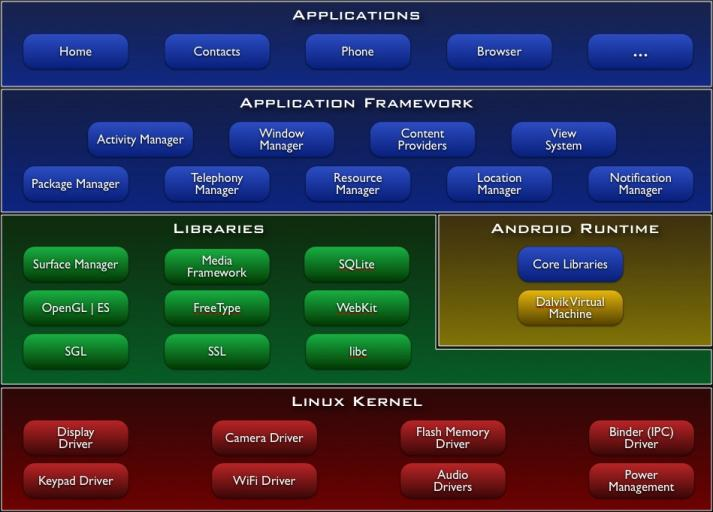
\includegraphics[width=0.8\textwidth]{android_systemarchitektur}
			      \caption{Die Android-Systemarchitektur}
			      \label{fig:android-system}
	% ''What is android?'' zuletzt besucht - 11.2010. [Online].
	% Available: http://code.google.com/android/what-is-android.html
			\end{figure}
	
	        \begin{quote}
	        ``Die DVM und JVM sind grob gesehen sehr �hnlich, wobei sie sich aber in
	        zwei Hinsichten grundlegend unterscheiden: Die DVM ist nicht als
	        Stack-Maschine, sondern als Register-Maschine realisiert, und die
	        L�ngen der Opcodes betragen bei der DVM zwei anstatt nur einem Byte.
	        Eine auf Register basierte virtuelle Maschine holt ihre Bytecodes und
	        Operanden aus (virtuellen) Registern. Dazu ist es nat�rlich
	        erforderlich, dass die Operanden in Abh�ngigkeit des Opcodes in
	        bestimmte Register geschrieben und von dort gelesen werden und nicht
	        generell vom Stack geholt werden, wie es in einer Standard JVM
	        geschieht." [Fokus09] 
	        \end{quote}
	
			Der Vorteil daraus ist schnell ersichtlich. Bei den Registern handelt es sich
			n�mlich quasi um Zwischenspeicher direkt im Mikroprozessor, die die
			Berechnungen �ber mehrere Zwischenergebnisse stark beschleunigen. 
			
			Da die Java-VM und der original Java-Bytecode lizenzrechtlich gesch�tzt sind,
			bediente sich Google eines Tricks, diese aussen vorlassen zu k�nnen. Die DVM
			wird nicht explizit als Java-VM dargestellt und verarbeitet keinen
			Java-Bytecode, sondern Android-eigenen Dex-Bytecode, der nicht unter die
			Sun-Lizenz f�llt. Es wird also gewohnterweise in Java programmiert und mit
			Hilfe des Java-Compilers von Sun Bytecode in Form von .class-Dateien erzeugt.
			Das Android eigene dx-Tool liefert aus dieser Quelle den Dex-Bytecode,
			der in eine f�r Android-Ger�te ausf�hrbare .apk-Datei (sprich fertig
			ausf�hrbare Anwendung) gepackt wird. Da die Programmierschnittstelle der Java
			SE von SUN bisher noch nicht patentrechtlich gesch�tzt ist, werden hier somit
			keine Rechte verletzt.
			
			\subsection{Android-Komponenten}
			
			Android stellt eine moderne Plattform f�r komponentenbasierte
			Anwendungsentwicklung dar. Hintergrund hiervon ist, dass f�r jede neue
			Applikation, die entwickelt werden soll das Rad nicht neu erfunden werden
			muss. Komplette Anwendungen oder Teile dieser sollen auch in neu
			entwickelten Anwendungen benutzbar sein. Erkl�ren l�sst sich dies an einem
			Beispiel: 
			
			Vorinstalliert auf einem Standard Android-Ger�t findet man Anwendungen wie
			``Kontakte'' oder ``Telefon''. In diesen Anwendungen sind beispielsweise
			Telefonnummern und Kontaktdaten gespeichert. M�chte man nun die Daten aus den
			Anwendungen benutzen kann man �ber die Datenbank der entsprechenden App
			(vorhandene Berechtigung vorausgesetzt) direkt auf die ben�tigten Werte
			zugreifen.
			
			Sauber gliedern sich die einzelnen Android-Komponenten gem�� dem in der
			Programmierung als Standard geltenden Model-View-Controller-Prinzips. %TODO:
			%ref anhang!
		
			\textbf{``Activity''} �bernimmt hier die Funktion des Views.
			Oberfl�chenelemente anzeigen, auslesen von Eingabefeldern und Benutzereingaben werden von den
			Activities behandelt. Man spricht hier von allen sichtbaren Bestandteilen
			einer Anwendung.
			
			F�r die Hintergrundprozesse ist im Android-Ger�t der \textbf{``Service''}
			zust�ndig. Analog zum Model-View-Controller-Prinzip w�rde man hier vom Controller
			sprechen. Wichtig sind diese Services zum Beispiel, wenn Prozesse
			weiterlaufen sollen, obwohl die Anwendungen vom Benutzer schon geschlossen
			wurden (Beispiel Musik Player).
			
			Das Model ist im Allgemeinen f�r die Verwaltung der darzustellenden Daten
			zust�ndig. Bei der Datenpersistenz in Android spricht man von
			\textbf{``Content Provider''}. �ber Berechtigungen k�nnen seine Daten
			bestimmten Anwendungen zur Verf�gung gestellt werden.
			
			Zus�tzlich zu den Standardkomponenten im MVC haben wir bei Android
			noch den \textbf{``Broadcast Receiver''}. Dieser empf�ngt Systemmeldungen z.B.
			�ber St�rungen des Netzwerks. Anwendungen haben so die M�glichkeit, auf einen
			ge�nderten Systemzustand zu reagieren.
	
			
			\subsection{Sicherheit}
			
			Das Sandbox-Prinzip: 
			\begin{quote}
	        ``Android f�hrt Anwendungen in der Sandbox aus. Eine Sandbox ist eine
	        eingeschr�nkte Laufzeitumgebung, in der bestimmte Funktionen verboten
	        sind.'' [BeckerPant10], S. 27
	        \end{quote}
	
			Eine Android-Anwendung besitzt aus der Sandbox heraus folgende Eigenschaften:
			\begin{itemize}
	          \item eigener Prozess
	          \item f�r einen eigenen Betriebssystem-User
	          \item eigene DVM
	          \item eigener Bereich im Hauptspeicher (Heap)
	          \item eigener Bereich im Dateisystem
	        \end{itemize}
			 
	        Wird eine Anwendung gestartet, l�uft sie unter dem Userkonto in einem
	        eigenen Prozess. Programme sind in Linux gegen den Zugriff von au�en
	        gesch�tzt, und dadurch kann auch kein unerlaubter Zugriff auf den
	        Speicher der DVM erfolgen, die in diesem Prozess l�uft.
	        
	        \subsection{Entwicklung}
            
            Prinzipiell ist man bei Android weder an Hardware noch Software zum
            entwickeln gebunden. Empfohlen wird allerdings die Eclipse IDE mit
            dem ADT Plugin.[ANDEV10], letzter Abruf 01.12.2010\\ Das Android
            SDK kann dann entweder von Hand �ber die Konsole zum erzeugen
            eines Projekts benutzt werden oder eben komfortabel �ber die IDE.
            Anwendungen f�r die Androidplattform werden ausnahmslos in Java
            geschrieben.
            
            %TODO: aufgeh�rt, morgen weiterschreiben!

            
		\section{Windows Phone 7}
		Relativ neu auf dem Markt ist das Windows Phone 7 (Verkaufsstart in
		Deutschland: 3. November 2010). [Heise10], letzter Abruf 30.11.2010\\ 
		Damit will Microsoft sein leicht angestaubtes Mobilbetriebssystem auf den
		neuesten Stand bringen und zu iOS und Android aufholen. Erste Testberichte
		zeigen, dass Windows Phone 7 bis jetzt ein zweischneidiges Schwert ist.
		
		Microsoft ist es gelungen eine einfach zu bedienende Oberfl�che zu
		erstellen, die sich von iOS und Apple abhebt. Den signifikanten Unterschied
		stellen die ``Live Tiles'' dar. Diese sind in verschiednen Gr��en auf dem
		Home Bildschirm darstellbarer Inhalt, der quasi live mit Informationen
		aktualisiert wird.
		
		Ausserdem stellt Microsoft klare Anforderungen an die Hardware f�r sein
		Betriebssystem. Windows Phone 7 ben�tigt einen Prozessor mit mindestens 1
		GHZ Taktfrequenz und einen internen Speicher von 8 GB. Dementsprechend
		fl�ssig und ohne Verz�gerung laufen auch die meisten Anwendungen auf den
		Ger�ten, die den hohen Auflagen gen�gen.
		
		Programmiert wird hier in Silverlight beziehungsweise XNA. Silverlight ist
		aus dem WPF (Windows Presentation Framework) heraus entstanden und auf
		verschiedenen Plattformen und Browsern lauff�hig. Das XNA Game Studio wurde
		in der Vergangenheit f�r die Entwicklung von Spielen auf dem PC bzw. der
		XBOX 360 benutzt. 
		
		Zumindest die Entwicklung mit dem XNA Game Studio ist kostenlos und wird als Add
		On f�r das Visual Studio 2010 Express verwendet. Als Entwicklungsplattform ist
		Microsoft also �hnlich strikt wie Apple angesiedelt und l�sst dies nur auf dem
		eigenen Betriebssystem zu.
						
		\section{Symbian}
		
		%evtl. noch Meego bzw. Maemo
		
		Entwickelt wird auf Symbian mit dem Qt SDK, welches f�r Windows,
		Linux oder Mac OS X verf�gbar ist. Alternativ l�sst sich auch der
		Eclipse-Ableger Carbide verwenden. Programmiert wird in C++. In Nokias Ovi
		Store kann die eigene Applikation vertrieben werden. Entwickler k�nnen sich
		in diesem f�r einmalig 50 Euro anmelden.
		
		Wie bereits erw�hnt befindet sich das Betriebssystem Symbian auf dem
		absteigenden Ast. Der Ansatz von Nokia das Betriebssystem seit dem 24. Juni
		2008 unter der Open-Source-Lizenz zu ver�ffentlichen f�hrte leider nicht mehr
		dazu, dass es wesentlich popul�rer wurde. Zu lange haben Nokia \& Co.
		gewartet.
		
		Nur noch bis zum 17. Dezember 2010 werden die Internetsites von Symbian mit
		Hilfen, Artikeln, FAQs, Tipps, Tricks und Historie online sein. Damit
		beendet Nokia seine Web-Pr�senz f�r die Open Source-Entwicklung. Die Daten
		sollen, so die Symbian Foundation, aber auch weiterhin erh�ltlich sein. Das
		ist offiziell das sichtbare Ende der Symbian-Unabh�ngigkeit und der Neustart
		unter der �gide des Mutterkonzerns Nokia. Nokia gab bekannt, dass ``aufgrund der
		Marktentwicklung die Weiterf�hrung des Projekts nicht mehr sinnvoll'' sei.
		[Symbian10], letzter Aufruf: 02.12.2010
		
		In Zukunft sollen Mobiltelefone von Nokia mit MeeGo angetrieben werden, einem
		offenen Linux-System, das seine Wurzeln einerseits in Nokias Maemo und
		andererseits in dem von Intel initiierten Moblin hat. [CT10], Seite 93
			
		\section{BlackBerry OS}
		
		F�r Blackberrys gibt es vergleichsweise wenige Apps. Dies liegt sicher daran,
		dass diese Ger�te h�ufig dienstlich genutzt werden und viele Firmen die
		Installation von Dritt-Anwendungen einschr�nken und/oder verbieten.
		
		Research In Motion (kurz RIM) setzt auf das im Vergleich zu aktuellen
		Java-Versionen abgespeckte Java ME. Dies entspricht ungef�hr dem Stand von
		Java SE 1.3, allerdings mit zus�tzlichen Bibliotheken f�r die Entwicklung
		von Software bei Mobiltelefonen.
		
		Empfohlen wird die Entwicklung mit Eclipse und einem entsprechenden Plug-in.
		Testen l�sst sich die selbstgeschriebene Applikation mit einem Simulator f�r
		fast jedes Ger�t von RIM. Allerdings ist der Zugriff auf viele APIs nur mit
		einer digitalen Signatur m�gliche. Diese l�sst sich RIM einmalig mit 20 \$
		finanzieren. M�chte man seine selbstgeschriebene Applikation im RIM eigenen
		Appstore vertreiben werden noch einmal 200 \$ f�llig.
		
		\section{HP webOS}
		
		Palm setzt mit seinem Betriebssystem auf Webstandards. Apps werden mit
		JavaScript, HTML5 und CSS geschrieben. Auch hier findet das MVC Prinzip
		einzug. Views werden als normale HTML-Dateien erstellt (mit Palm-propriet�ren
		Attributen und Styles). Controller werden mit Hilfe von JavaScript-Klassen
		dargestellt mit definierten Einstiegspunkten und Callbacks. F�r die
		Persistenzschicht zum dauerhaften Speichern der Daten stehen HTML5-konforme
		APIs und SQLite-Datenbanken zur Verf�gung.
		
		Das WebOS-SDK iust f�r Windows, Mac OS X und Linux verf�gbar. Zus�tzlich
		bietet Palm ein Eclipse-Plug-in zum einfachen Packen und starten der
		Anwendung aus der IDE sowie der freien Virtualisierungssoftware VirtualBox
		basierenden Emulator. Alternativ kann mittels ``Ares'' im Webbrowser
		entwickelt werden. Dieser besteht aus einer Projekt-Verwaltung, einem
		JavaScript-Editor und einem WYSIWYG-Editor.
		
		Fertige Anwendungen werden nicht signiert und liegen im Quellcode vor. Dies
		ist nicht ganz unkritisch, da diese leicht entpackt und ver�ndert werden
		k�nnen, zum Beispiel zum aushebeln von Sicherheitsmechanismen, indem einfach
		die spezielle JavaScript-Zeile auskommentiert wird.
		
		Die zuvor festgelegte Geb�hr in h�he von 99 \$ zur Teilnahme am
		Entwicklerprogramm hat Palm ausgesetzt. Von daher entstehen im Moment keine
		zus�tzlichen Kosten bei der Entwicklung bzw. beim Publishing im Market.
		
		\section{WebApp}
		
		%TODO: Holperdistolper und unvollst�ndig
		Eine schnell umzusetzende Applikation f�r alle verf�gbaren Betriebssysteme
		im Mobilbereich w�re eine Browserbasierte L�sung. Diese kann nat�rlich f�r
		mobile Ger�te im Hinblick auf Darstellung und Benutzbarkeit optimiert werden.
		
		Die Entwicklung w�rde sehr schnell von statten gehen, da die benutzte Technik
		weit verbreitet ist und g�ngige Browser im Mobilbereich die Standards der
		Webprogrammierung unterst�tzen.
		
		Leider ist es dabei aber nicht m�glich auf die ger�tespezifischen
		Eigenschaften zuzugreifen. Es gibt zwar Ans�tze wie beispielsweise Sencha
		Touch, in der sich das Userinterface den entsprechenden Ger�ten anpassen
		l�sst, aber Kamera, GPS \& Co. sind aus Sicherheitsgr�nden nicht �ber ein
		Webinterface ansprechbar (Einzig Lokalisierungsdienste wie Google bieten hier
		eine Ausnahme). So ist die Entwicklung einer WebApp doch relativ beschr�nkt und nur
		f�r Anwendungen zu benutzen, die nicht auf die Hardware des Ger�ts zugreifen m�ssen. 
		
		Eine gute Kombination aus WebApp und nativen Apps bieten Cross-Platform
		Development Tools, welche im Folgenden beschrieben werden.
		
					
		\section{Cross-Platform Development Tools}
            
            Unter Cross-Platform development versteht man im Allgemeinen ein
            Framework, das es erm�glicht Applikationen auf mehreren Endger�ten zu
            deployen. Im Vordergrund steht nicht die Performance der Anwendung,
            sondern die Kompatibilit�t mit verschiedenen Betriebssystemen und deren ``look
            and feel'' so nahe wie m�glich zu kommen. [CT10], S. 96
            
            Zur Zeit befinden sich die Frameworks
            PhoneGap\footnote{http://www.phonegap.com},
            Titanium\footnote{http://www.appcelerator.com/} und
            Rhodes\footnote{http://rhomobile.com/} (evtl. + Sencha Touch) sich
            auf dem Markt. All diese basieren auf Webtechniken und zielen
            speziell auf Webentwickler ab, da diese ihre F�higkeiten direkt
            f�r die Smartphone Apps Welt benutzen k�nnen (Vgl. Tabelle \ref{tab:cross-platform}).
            
            PhoneGap und Titanium werden mit Hilfe von HTML, CSS und JavaScript
            programmiert. Beide benutzen JavaScript APIs, um auf die nativen
            Ger�tefunktionen des Smartphones zugreifen zu k�nnen
            (Beispielsweise GPS, Accelerometer, Sound). Im Gegensatz dazu wird
            in Rhodes mit Ruby gearbeitet. Es bietet eine komplette
            Serverumgebung auf dem Ger�t und dadurch Zugriff auf die nativen
            Funktionen.
            
            PhoneGap und Titanium greifen �ber bestimmte JavaScript APIs auf
            die Funktionen der Smartphones zu. Die Logik (HTML, CSS,
            Javascript) wird allerdings in einem Browserfenster angezeigt.
            Durch die JavaScript APIs hat die ``Web App'' sozusagen Zugriff auf
            alle interessanten Funktionen des Handys, wie zum Beispiel die
            Geolocation, das Accelerometer, die Kamera, Kontakte, Datenbank
            oder das File System.
			
			Prinzipiell kann jede Funktion, die das Smartphone SDK anbietet in die
			Javascript Welt �berf�hrt werden. Eine normale Web App, die im mobilen
			Browser des Handys l�uft k�nnte zum Beispiel nicht auf diese Funktionen
			zugreifen (Sicherheitsaspekt).
			
			Auf der Titanium Webseite wird damit geworben, dass daf�r entwickelte
			Anwendungen in native Anwendungen f�r das zu entwickelnde System kompiliert
			werden k�nnen. Man darf das allerdings nicht falsch verstehen. Titanium kann
			kein HTML, CSS oder JavaScript in nativ geschriebene Anwendungen umwandeln.
			Diese werden einfach als Ressourcen zu der ausf�hrbaren App hinzugef�gt. Am
			besten stellt man es sich so vor, wie ein eingebettetes Bild. Wenn die App
			ausgef�hrt wird, werden diese Ressourcen in den ``UIWebView'' geladen und als
			JavaScript ausgef�hrt.
	
			Genau so wird es auch in PhoneGap gemacht. Hinsichtlich Architektur sind
			sich beide Frameworks sehr �hnlich. Ein wesentlicher Unterschied ist, dass
			PhoneGap nicht die nativen Userinterfacekomponenten in JavaScript zur
			Verf�gung stellt. Das ``Look and Feel'' muss mittels CSS selbst aufbereitet
			werden. Im Gegensatz dazu bietet Titanium eine starke UI API, die mittels
			JavaScript dazu benutzt werden kann alle m�glichen Arten von nativen UI
			Kontrollen zu erzeugen. Im direkten Vergleich sehen deswegen Titanium Apps
			eher wie direkt f�r das Smartphone geschriebene Apps aus. Allerdings
			unterst�tzt PhoneGap mehr verschiedene Betriebssysteme als Titanium. Die
			PhoneGap APIs sind allgemeiner gefasst und k�nnen so auf vielen
			verschiedenen Systemen wie z.B. iPhone, Android, Blackberry oder Symbian
			laufen. Titanium konzentriert sich auf das iPhone und den Android Markt.
								
			Mit Hilfe des Rhodes Frameworks wird es Entwicklern gestattet native Apps zu
			erstellen mit der M�glichkeit HTML Templates zu erstellen und in Ruby zu
			programmieren. Apps, die mit Rhodes entwickelt werden haben die Performance
			und die F�lle von Apps, die nativ f�r das entsprechende System geschrieben
			wurden mit dem Vorteil, dass das Interface in HTML verfasst wird. Ausserdem
			sehr positiv f�llt auf, dass Rhodes das MVC Prinzip verwendet und somit
			Logik und Anzeige strikt getrennt sind.
			
			Entwickler mit Railserfahrung werden sicherlich schneller mit Rhodes
			zurechtkommen. Das Framework hat �brigens auch Grenzen. Diese manifestieren
			sich vor allem darin, dass es keinerlei Integration von Audio oder Video in
			den einzelnen Apps gibt. Rhodes bietet auch an, dass man Funktionen aus den
			nativen APIs des Systems aufrufen kann, wenn diese nicht im Framework
			unterst�tzt werden sollten. Jedoch sollte man sich nicht darauf verlassen,
			dass diese dann fl�ssig ablaufen.

			Worin sich jedoch alle Produkte voneinander abheben ist die
			Entwicklerlizenz. PhoneGap ist Open-Source und kann frei genutzt werden.
			Titanium befindet sich noch im Betastadium, wird aber in Zukunft ein
			kommerzielles Produkt werden. Rhodes ist bereits kommerziell und kostet 500
			\$ pro Projekt. Die Summe muss vor Beginn der Entwicklung bezahlt werden.
			
	        \begin{table}%[h]
	        	\centering \leavevmode %Tabelle zentrieren
		        \caption{JavaScript-Frameworks f�r mobile
		        Apps}\footnotemark
		        \label{tab:cross-platform}
		        %\addtocounter{footnote}{+1}
		        \begin{tabular}{|l|l|l|l|}
		        \hline
		        Name & PhoneGap & Titanium Developer & Rhodes\\
		        \hline
		        \hline
		        App-Typ & quasi-nativ & quasi-nativ & (quasi-)nativ\\
		        \hline
		        Hersteller & Nitobi & Appcelerator & Rhomobile\\
		        \hline
		        Betriebssysteme & alle(Eclipse) & Windows, Linux, Mac OSX & Windows,
		        Mac OSX\\
		        \hline
		        Lizenz & MIT & Apache & MIT\\
		        \hline
		        Programmiersprache & JavaScript & JavaScript & Ruby\\
		        \hline
		        Plattformen & & &\\
		        \hline
		        \hline
		        Android & $\surd$  & $\surd$  & $\surd$ \\
		        \hline
		        iPhone & $\surd$ & $\surd$ & $\surd$\\
		        \hline
		        WebOS & $\surd$ & x & x\\
		        \hline
		        Symbian & $\surd$ & x & $\surd$\\
		        \hline
		        Blackberry & $\surd$ & $\surd$(nur Pro-Version) & $\surd$\\
		        \hline
		        Windows Mobile & $\surd$ & x & $\surd$\\
		        \hline
		        \end{tabular}
			\end{table}
			%\addtocounter{footnote} 
			\footnotetext{[CT10], S. 101}
			
% 		\subsection{atvise}		
% 		\begin{itemize}
%           \item Web-basierte L�sung. 1 Server f�r alle Ger�te mit Browser
%           \item Wirbt f�r Mobile Endger�te (speziell auch iPhone)
%           \item Darstellungsfehler im Safari beim surfen auf der LiveDemo mit
%           dem iPhone
%           \item iPhone Safari st�rzt bei animierter Darstellung ab?!?
%         \end{itemize}


\chapter{Implementierung und Test}%Softwareerstellung}
		\section{Wahl des Betriebssystems}
		\begin{itemize}
          \item tja\ldots Entweder nur eins ausw�hlen oder Android und iOS und
          Win7 Mobile (oder Webinterface\ldots) -> ZU VIEL ARBEIT?
          \item Wahrscheinlich muss die Entwicklung f�r iOS ausgeschlossen
          werden, weil die entsprechende Entwicklungshardware fehlt. ODER:
          JAILBREAK -> Eclipse -> TESTEN LIVE AUF DEM GER�T OHNE SIMULATOR
          (zumindest theoretisch auf diese M�glichkeit eingehen).
          \item gibt es evtl. freie iphone emulatoren? ->derzeitige Recherche->
          NEIN
          \item Entwicklungsumgebung f�r Android und Win7 Mobile ist kostenlos.
          \item Annahne: Wahrscheinlich f�llt die Wahl auf Android, da hier
          auch direkt auf einem Ger�t getestet werden kann und nicht nur auf
          dem Simulator. Zu demonstrationszwecken ist dies wohl sinnvoller. 
        \end{itemize}
        \section{Codegenerierung}
        
        \subsection{Vorhandene Tools auf dem Markt}

      Verzichtet werden soll auf die Verwendung kommerziell-, propriet�rer
      Software zugunsten offener Standards und frei verf�gbarer
      Open-Source Technologien. Dabei sind auch �berlegungen zu den
      unterschiedlichen Lizenzen anzustellen.
      
      Deswegen werden im Folgenden erst grafische Tools zur Modellierung der
      Diagramme untersucht und anschlie�end Transformationstools, die f�r die
      �berf�hrung der einzelnen Modelle und schliesslich f�r den entstehenden
      Quellcode verantwortlich sind.
      
 	  \subsubsection{Visual Paradigm}
      
      Visual Paradigm ist sehr leicht und intuitiv zu erlernen. Die meisten
      Funktionen findet man auf anhieb, ohne auch nur einen Blick in die
      Dokumentation werfen zu m�ssen. Allerdings macht das arbeiten mit Visual
      Paradigm in Kombination mit einem Transformationstool nicht
      viel Sinn, da beim Export der Diagramme in XML Files Informationen verloren
      gehen. Beim Import in Acceleo beispielsweise fehlen die Namen bzw.
      Bezeichnungen der Diagramme so wie Zusammenh�nge der einzelnen
      Diagrammarten, die jedoch vorher definiert wurden. Damit ist Visual
      Paradigm f�r den Zweck der Codegenerierung relativ unbrauchbar.

      \subsubsection{MagicDraw}

      Ein erster Versuch ein einfaches Klassendiagramm zu implementieren und in
      Code umzuwandeln klappte erstaunlicherweise recht gut. Allerdings ist die
      Bedienung von MagicDraw wesentlich komplexer und un�bersichtlicher als bei
      Visual Paradigm. Die Einarbeitungszeit ist bei dieser Komplexit�t
      exponentiell gr��er. Daher verz�gerte sich die Erstellung der Diagramme
      sehr. Was in Visual Paradigm in Stunden machbar war, dauerte hier
      einen ganzen Tag. Schlechte Navigation, un�bersichtliche Men�s und
      unzureichende Dokumentation zur Software, aber daf�r volle
      Kompatibilit�t zum XML Standard.
      
      \subsubsection{Acceleo}
      
      Einfache Klassendiagramme in Code umzuwandeln ist mit dem Tool kein
      Problem. Allerdings ist die Dokumentation in Bezug auf Diagrammarten
      ziemlich unvollst�ndig. Das Durchlaufen von Aktivit�tsdiagrammen ist
      prinzipiell anhand der Activities m�glich. Allerdings konnte ich nicht
      herausfinden, wie man diese in der richtigen Reihenfolge darstellt.
      Acceleo wirft die Ergebnisse einfach so durcheinander, in der Reihenfolge
      wie sie im XML File des UML's generiert wurden. Aus einem Kontrollfluss
      heraus etwas zu erzeugen stellt sich also als ziemlich unm�glich dar.
      
      \subsubsection{oAW}
        
        \begin{itemize}
          \item Probleme w�hrend der Umsetzung?
          \item Erwartungshaltung?
          \item Umsetzung aus AndroMDA heraus
        \end{itemize}
        \section{Tests White/Blackbox?}
        \begin{itemize}
          \item Testf�lle aufstellen und diese mit JUnit umsetzen(nur f�r
          Android)
          \item Alternatives Testframework f�r iPhone \& Win7 Mobile?!?
        \end{itemize}
%Zukunftsausblick und Zusammenfassung der Arbeit
\chapter{Zusammenfassung und Ausblick}

\begin{itemize}
  \item 2-3 Seiten Zusammenfassung der Arbeit und Ausblick auf weitere
Projekte f�r die Zununft
  \item Vgl. Erwartete Ergebnisse - Abweichungen  
  \item marketingtechnische konzepte: kann das ergebnis im hinblick darauf
  kontrolliert werden? kundenzufriedenheit \& co.? wie k�nnte eine m�gliche
  evaluation erfolgen?
\end{itemize}

Die Erwartungshaltung f�r diese Diplomarbeit bestand darin in einer vorgegebenen
Zeit zu evaluieren, ob der Einsatz von Smartphoneapps in der Kommunikation mit
Maschinen lohnend ist oder nicht. Ausgehend vom Wissensstand zu Beginn dieser
Arbeit wurde vermutet, dass die Umsetzung einer App durchaus m�glich, wenn
auch nicht einfach ist. Die gr��te Schwierigkeit im Vorfeld lag vor allem daran,
die Darstellung der verschiedenen Funktionen f�r das Endger�t so zu optimieren,
dass die Lesbarkeit der Information jederzeit gew�hrleistet sein sollte. Bei
einer begrenzten Displaygr��e vor allem bei Smartphones m�ssen Informationen
klar und deutlich zu gewinnen sein. 

% \clearpage
% \thispagestyle{empty}
% \begin{figure}[hp]
% 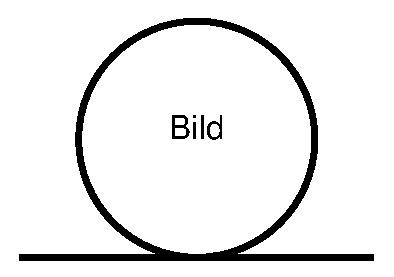
\includegraphics[width=\textwidth]{beispiel}
% \end{figure} 
% \clearpage
% 
% \chapter{Beispielanhang 2}
% Dies ist das Deckblatt. Es sollte die kurze Beschreibung der n�chsten Seite enthalten. Der Titel ist meist ausreichend.
% 
% % so gehts auch
% \clearpage
% \thispagestyle{empty}
% \begin{figure}[hp]
% 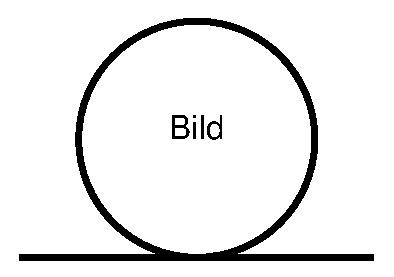
\includegraphics[height=\textwidth,angle=90]{beispiel}	% jetzt querformat
% \end{figure} 
% \clearpage
% 
% \addtocontents{toc}{\vspace{-1ex}}
% \chapter{Beispielanhang 3}
% Dies ist das Deckblatt. Es sollte die kurze Beschreibung der n�chsten Seite enthalten. Der Titel ist meist ausreichend.
% 
% 
% % Wenn der Anhang als PDF vorliegt kann man ihn einfach so einf�gen: (Paket pdfpages n�tig)
% \ifpdf % funktioniert leider nur mit pdfLaTeX 
% 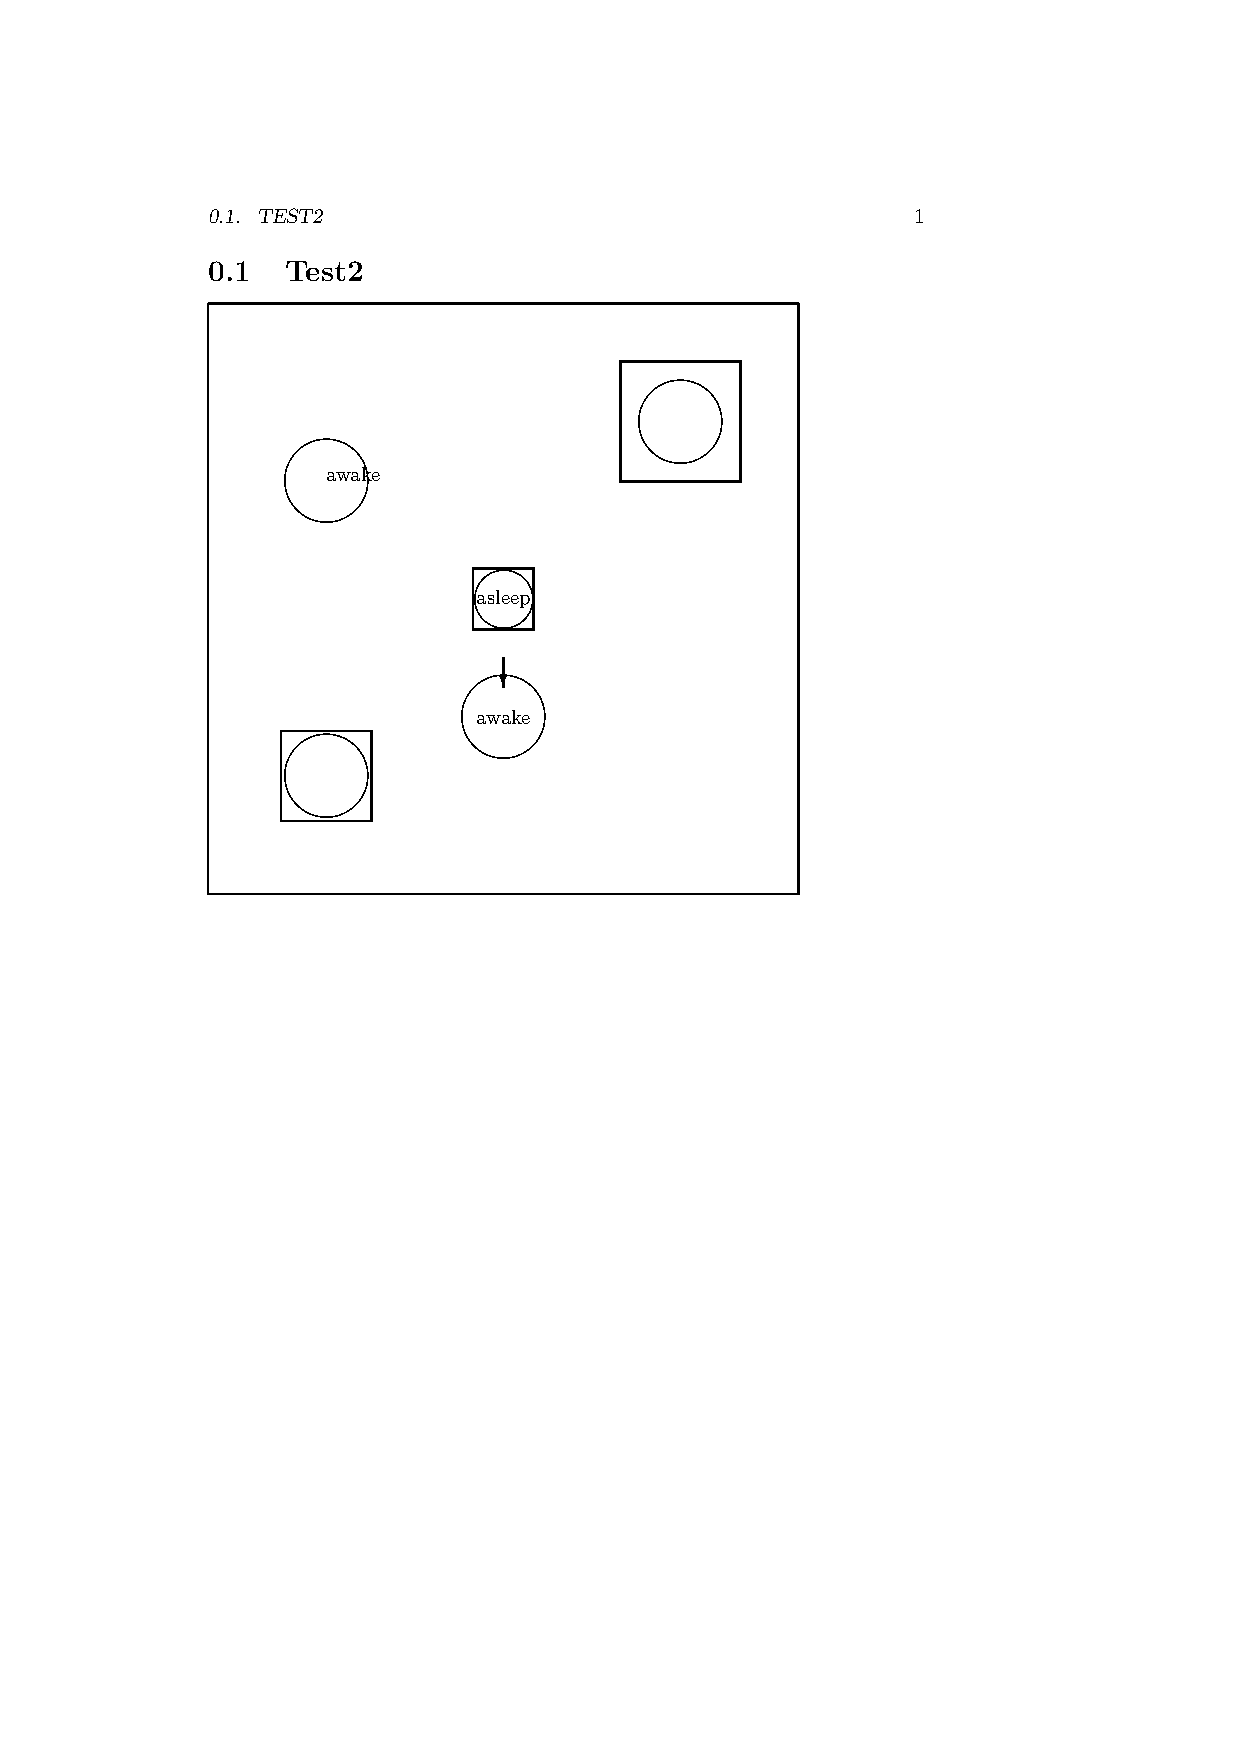
\includepdf[pages=-]{anhang/beispielanhang}	% pages=- bedeutet: alle Seiten | Wie bei Bilder die Dateierweiterung (.pdf) am besten weglassen
% % Weites Beispiel: Nur Seiten 1-2 und 4, Papier querformat mit 2 Seiten pro Seite
% %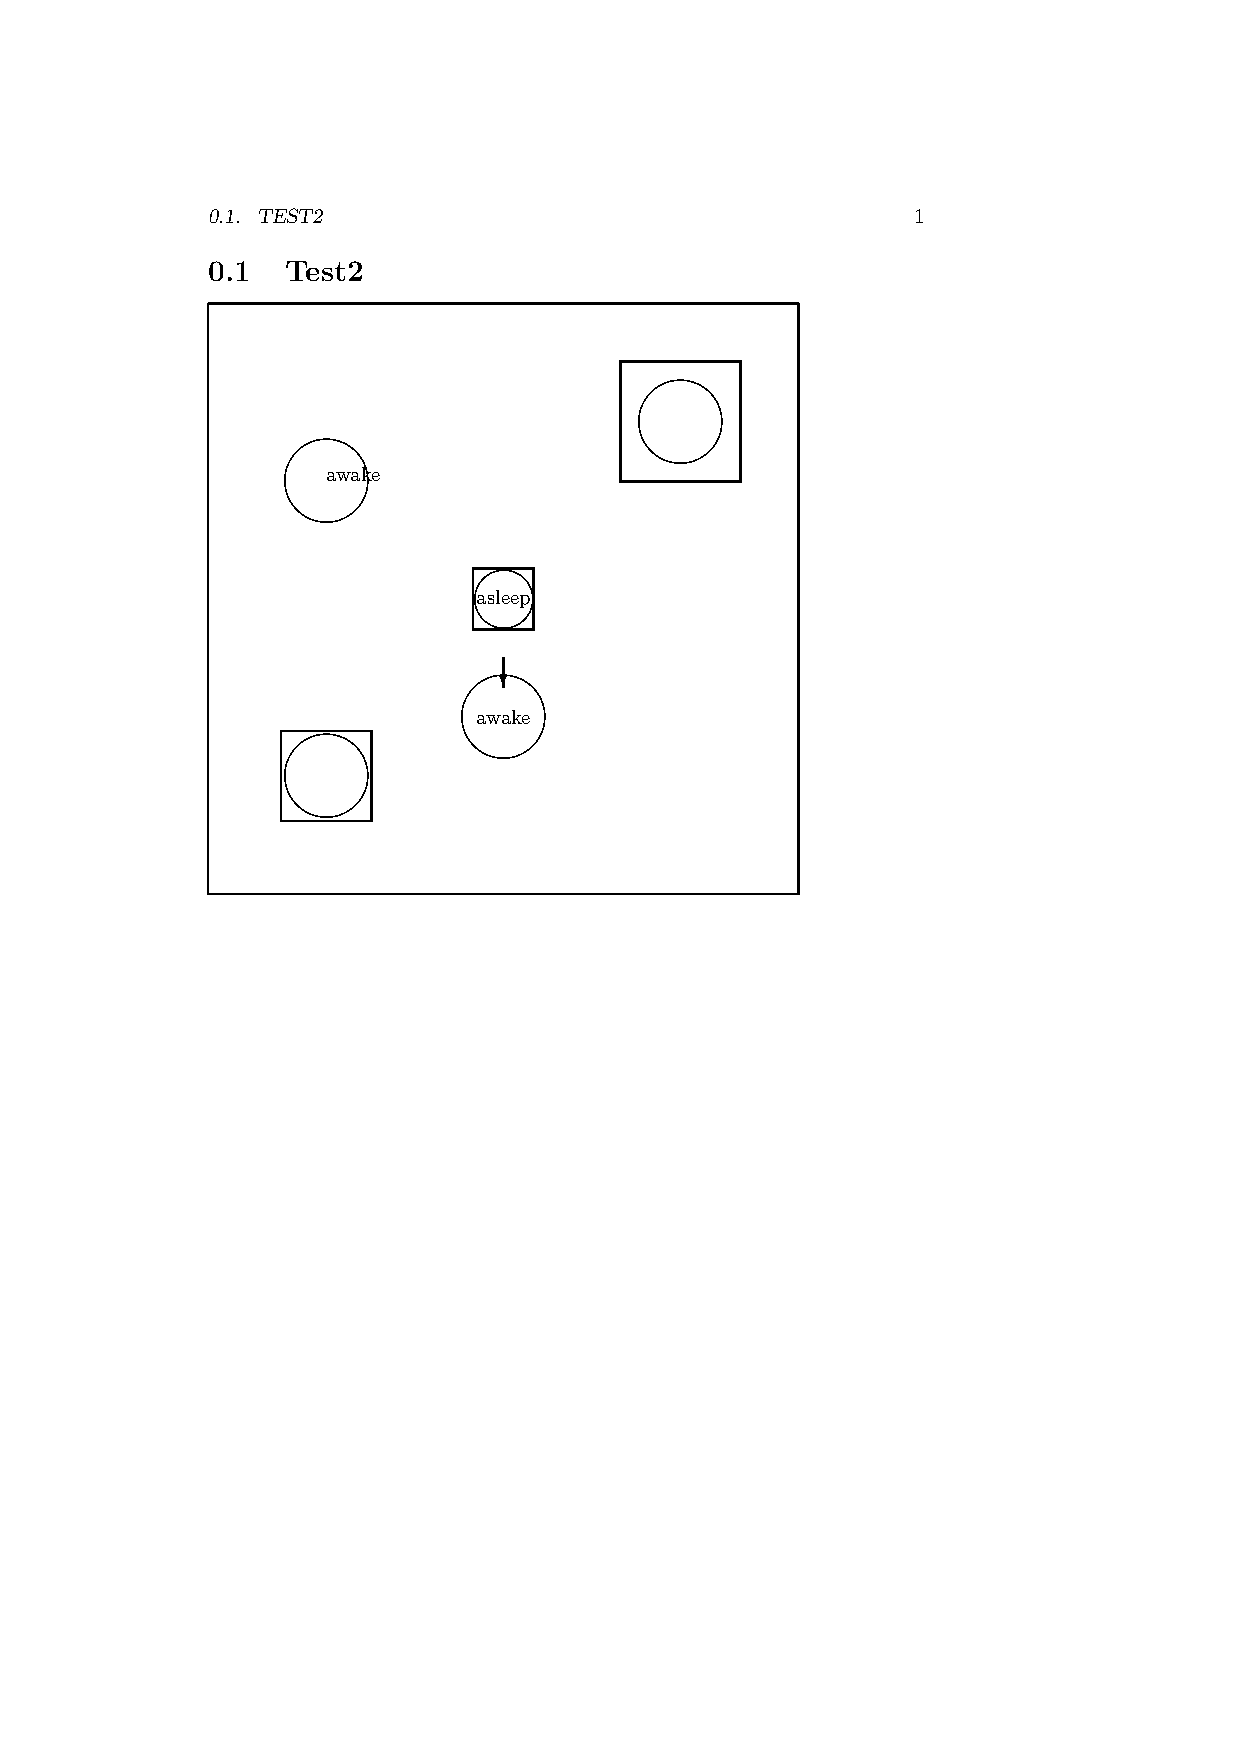
\includepdf[pages={1-2,4},landscape,nup=1x2]{anhang/beispielanhang}
% 
% \else  % bei der Verwendung vom normalen LaTeX:
% \newpage
% \addtocounter{page}{5}	% Seitenz�hler hochz�hlen und Anhang nach dem Drucken manuell hinzuf�gen
% % Hier wurde angenommen, dass der Anhang f�nf Seiten lang ist
% \fi
% 
% \chapter{Weiterer Anhang}

%ANHANG TODO: BUCHSTABEN statt Zahlen... aber wie??
\begin{appendix}
%Literaturverzeichnis
%try mit bibtex

\begin{thebibliography}{99}
\addcontentsline{toc}{chapter}{Literaturverzeichnis}

% \begin{flushleft}
% 	
% 	\bibliographystyle{alpha}
% 	\bibliography{referenzen}
%  	
% \end{flushleft}

\bibitem{Clark10} [Clark10] Josh Clark: Tapworthy - Designing Great iPhone
Apps, 1. Auflage, O'Reilly 2010

\bibitem{Broy10} [Broy10] Manfred Broy: CYBER-PHYSICAL SYSTEMS - Innovation
durch softwareintensive eingebettete Systeme, 1. Auflage, Springer 2010

\bibitem{KHS10} [KHS10] o.V.: Unternehmen, In: KHS GmbH, Stand: 2010, URL:
http://www.khs.com/de/unternehmen.html

\bibitem{Gartner10} [Gartner10] Gartner: Technology Research \& Business Leader
Insight, In: Gartner, Inc., Stand: November 2010, URL:
http://www.gartner.com/it/page.jsp?id=1466313 (letzter Abruf am 17.11.2010)

\bibitem{CHI99} [CHI99] Fukumoto Masaaki: Whisper  - A Wristwatch Style
Wearable Handset, o.V., USA 1999 

\bibitem{Schmalenbach05} [Schmalenbach05] Jenni Schmalenbach: Das Ph�nomen
Short Message Service (SMS) - Einf�hrung in eine neue Kommunikationsform, 1. Auflage,
Ludwig-Maximilians-Universit�t M�nchen 2005

\bibitem{BeckerPant10} [BeckerPant10] Arno Becker, Marcus Pant: Android 2 -
Grundlagen und Programmierung, 2. Auflage, dpunkt.verlag 2010

\bibitem{Petzold10} [Petzold10] Charles Petzold: Programming Windows Phone 7, 1.
Auflage, Microsoft Press 2010

\bibitem{ITU10} [ITU10] o.V.: International Telecommunication Union, Stand:
15. Februar 2010, URL:
http://www.itu.int/net/pressoffice/press\_releases/2010/06.aspx

\bibitem{Apple10} [Apple10] o.V.: Apple Special Event, Stand: 20. Oktober 2010,
URL: http://events.apple.com.edgesuite.net/1010qwoeiuryfg/event/index.html

\bibitem{AppleDev10} [AppleDev10] o.V.: Apple Developer, Stand: 2010, URL:
https://developer.apple.com

\bibitem{Fokus09} [Fokus09] o.V.: Fokus Report, Fachhochschule Nordwestschweiz,
250. Auflage, Verlag: Fachhochschule Nordwestschweiz FHNW Institut f�r Mobile und Verteilte
Systeme

\bibitem{Heise10} [Heise10] o.V.: Heise Online, Stand: 20.10.2010, URL:
http://www.heise.de/newsticker/meldung/Windows-Phone-7-startet-bei-T-Mobile-mit-Verzoegerung-1121952.html

\bibitem{CT10} [CT10] o.V.: c't - magazin f�r computer technik, Heft 16,
Heise Zeitschriften Verlag GmbH \& Co. KG, Stand 19.07.2010

\bibitem{CT10_2} [CT10\_2] o.V.: c't - magazin f�r computer technik, Heft 20,
Heise Zeitschriften Verlag GmbH \& Co. KG, Stand 13.09.2010

\bibitem{ANDEV10} [ANDEV10] o.V.: Android Developers, Stand: 02.11.2010, URL:
http://developer.android.com/guide/developing/other-ide.html

\bibitem{Symbian10} [Symbian10] o.V.: Symbian Foundation, Stand: 28.11.2010,
URL: http://developer.symbian.org/wiki/Symbian\_Foundation\_web\_sites\_to\_shut\_down

\bibitem{Koller10} [Koller10] Dr. Dirk Koller: iPhone-Apps entwickeln -
Applikationen f�r iPhone, iPad und iPod touch programmieren, 1. Auflage,
Franzis Verlag, Poing, 2010

\bibitem{Eren06} [Eren06] Evren Eren, Kai-Oliver Detken: Mobile Security -
Risiken Mobiler Kommunikation und L�sungen zur Mobilen Sicherheit, 1. Auflage,
Carl Hanser Verlag, M�nchen, 2006

\bibitem{Radius10} [Radius10] o.V.: freeRADIUS - The world's most popular RADIUS
Server, Stand: 28.09.2010, URL: http://freeradius.org/

\bibitem{Stahl07} [Stahl07] Thomas Stahl, Markus V�lter, Sven Efftinge, Arno
Haase: Modellgetriebene Softwareentwicklung - Techniken, Engineering,
Management, 2. Auflage, dpunkt.verlag, Heidelberg, 2007

\bibitem{Gruhn06} [Gruhn06] Volker Gruhn, Daniel Pieper, Carsten R�ttgers:
Effektives Software-Engineering Mit UML2 und Eclipse, 1. Auflage,
Springer Verlag, Berlin Heidelberg, 2006



\end{thebibliography}

% Empfohlende Alternative: BibTeX oder BibLaTeX!!

% \begin{thebibliography}{99}
% \addcontentsline{toc}{chapter}{Literaturverzeichnis}
% 
% \bibitem{ImageNation}
%   \textsc{Imagenation Corporation}:
%   \textsl{User's Guide for the PX510 and PX610}.
%   ImageNation Systems, September 1997
% 
% \bibitem{platt}
%   \textsc{Platt, David S.}:
%   \textsl{The essence of COM and ActiveX: a programmers workbook}.
%   2nd~Edition, Prentice Hall, 1998
% 
% \bibitem{isernhagen}
%   \textsc{Isernhagen, Rolf}:
%   \textsl{Softwaretechnik in C und C++}.
%   2.~Auflage, Carl-Hanser-Verlag, 2000
% 
% \bibitem{sphar}
%   \textsc{Sphar, Chuck}:
%   \textsl{Visual C++ 6}.
%   Microsoft Press Deutschland, 1999
% 
% \bibitem{zamperoni}
%   \textsc{Zamperoni, Piero}:
%   \textsl{Methoden der digitalen Bildsignalverarbeitung}.
%   5.~Auflage, Springer-Verlag, 2002
% 
% \bibitem{url_directx}
%   \url{http://www.microsoft.com/windows/directx}\\
%   Microsoft DirectX Homepage
% 
% 
% \end{thebibliography}

%Anhang (Quellcode...)
\newpage
\chapter{Anhang}
%\addcontentsline{toc}{chapter}{Anhang}

%	\section{Vom Telefon zum Smartphone}
% 		\subsection{Entstehungsgeschichte}
% 		
%  		Die Geschichte des Telefons beginnt mit Alexander Graham Bell im Jahre 1876,
% 		dem Jahr in dem er das von Ihm entwickelte elektromagnetische Telefon zum
% 		ersten Mal au�erhalb seines Labors, in Boston, auf einer Versuchsstrecke von
% 		8,5 Km L�nge angewandt hat. Bell stellt sein verbessertes Telefon vor. Er
% 		l�sst es am 08. M�rz patentieren. 
% 		
% 		Einige Zeit sp�ter begann die Entwicklung des Mobilfunks. 1926 stellt die
% 		Deutsche Reichsbahn und Reichspost einen Telefondienst auf der Strecke
% 		zwischen Hamburg und Berlin zur Verf�gung, der Reisenden der 1. Klasse
% 		angeboten wird.
% TODO: evtl. in den Anhang? oder ganz raus... eigentlich irrelevant!


\section{Jailbreak}
%TODO: ausf�rhlichere Erkl�rung + Bilder

\subsection{Wikipedia Eintrag}

Seit dem 27. Juli 2010 ist die Entsperrung in den USA legal, die Rechtslage in
Deutschland ist bisher nicht eindeutig gekl�rt. 

Im Juli 2007 beschrieb der Norweger Jon Lech Johansen in seinem Blog, wie man
die Funktionen des iPhones auch ohne AT\&T-Vertrag nutzen kann.

Im August 2007 berichtete das Technik-Blog Gizmodo, dass sich das iPhone mit
Hilfe einer sogenannten ``Turbo-SIM-Karte'' auch in anderen GSM-Netzen betreiben
lasse. Am 6. September 2007 ver�ffentlichte die Webseite des APC Magazine
eine Zehn-Schritte-Anleitung zur Nutzung des iPhones in weltweit allen
GSM-Netzen mit Hilfe einer Turbo-SIM-Karte.

Ebenfalls im August 2007 gelang es dem US-Amerikaner George Hotz, ohne den
Umweg �ber eine Turbo-SIM-Karte die Beschr�nkung der Nutzung seines iPhones
auf das AT\&T-Netz aufzuheben. In seinem Blog beschrieb er dazu ein Verfahren,
das komplizierte Eingriffe in die Hardware erfordert.

Im September 2007 stellte das iPhone Dev Team, eine freie Gruppe von
Programmierern, eine Software-Netlock-Entsperrung f�r das iPhone frei im
Internet zur Verf�gung. Damit war das iPhone weltweit in allen GSM-Netzen auch
f�r iPhone-Besitzer nutzbar, die den technischen Aufwand bislang verf�gbarer
komplizierter Hacks gescheut hatten.

Einen Tag nach Release des iPhones 3GS wurde ein Tool zur Entsperrung dieses
Ger�tes ver�ffentlicht.

Am 22. Juni 2009 hat das iPhone Dev-Team eine rein softwarebasierte
SIM-Entsperrung namens ultrasn0w f�r alle iPhones ab Firmware 3.0
ver�ffentlicht, mit der die Ger�te in allen Netzen betrieben werden k�nnen.
Mit vielen Firmwarereleases kommen neue Versionen der Netzkontrollsoftware,
wodurch neue Exploits gefunden werden m�ssen, um diese erneut freizuschalten.
Bisher ist dies f�r jedes Baseband gelungen. Im Mai 2010 wurde das Tool Spirit
ver�ffentlicht, das auch f�r das iPad mit iOS 3.2 funktioniert.

Am 1. August 2010 wurde ein webbasierter Jailbreak namens JailbreakMe
ver�ffentlicht, mit dem auch das iPhone 4 ge�ffnet werden kann. Hierf�r wurde
ein Programmfehler bei der PDF-Darstellung im Programm Mobile Safari genutzt.
Am Tag darauf warnte das BSI davor, mit dem iPhone PDFs zu �ffnen, da auch ein
sch�dlicher Code ausgef�hrt werden k�nnte. Eine Apple-Pressesprecherin
verk�ndete, dass Apple den Fehler bereits behoben habe und schnellstm�glich
ein Update herausbringen werde.

Apple gab daraufhin am 11. August 2010 ein Update (iOS 4.0.2) heraus, das zwei
Sicherheitsl�cken schloss. Die eine L�cke betraf eine Systembibliothek
(``Freetype'') - durch die zweite erreichte das ausf�hrende Programm
System-Rechte am Ger�t.

\subsection{Anwendung}

Die konkreten Zielplattformen f�r den Prototypen wurden auf Android und iOS
festgelegt. Das Android Ger�t musste f�r die Entwicklung nicht modifiziert
werden. Bei dem Apple iPad war es n�tig, dieses zu Jailbreaken, um Anwendungen
darauf testen zu k�nnen. Nach R�cksprache mit der KHS wegen Garantieverlust und
Haftung durfte ich mich ans Werk machen.

\url{http://www.theiloop.com/how-to-jailbreak-ipad-running-ios-4-2-1-using-redsn0w-windows/}

tutorial f�r windows

noch nicht untethered verf�gbar... mal kucken. hauptsache cydia store geht

evtl. noch warten? 

bzw. zum testen pc mit redsnow n�tig, sonst tethered... aber ipad kann ja
jederzeit �ber itunes zur�ckgesetzt werden...

erstes auftretendes problem: kein itunes bei khs. 

auf dem eigenen rechner jailbreaken...

annahme: redsnow hack ist auch in der firma ausf�hrbar, um den cydia store zu
testen

\section{Hackint0sh}
%TODO: ausf�rhlichere Erkl�rung + Bilder

\section{Model-View-Controller-Prinzip}
%TODO: Erkl�rung + Bilder





% \clearpage
% \thispagestyle{empty}
% \begin{figure}[hp]
% 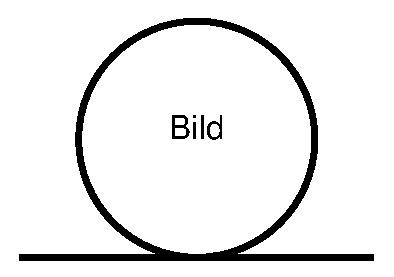
\includegraphics[width=\textwidth]{beispiel}
% \end{figure} 
% \clearpage
% 
% \chapter{Beispielanhang 2}
% Dies ist das Deckblatt. Es sollte die kurze Beschreibung der n�chsten Seite enthalten. Der Titel ist meist ausreichend.
% 
% % so gehts auch
% \clearpage
% \thispagestyle{empty}
% \begin{figure}[hp]
% 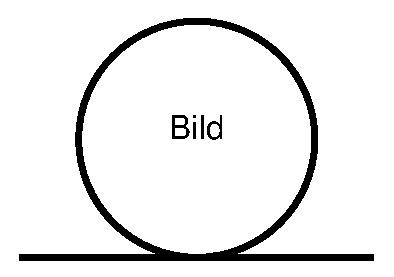
\includegraphics[height=\textwidth,angle=90]{beispiel}	% jetzt querformat
% \end{figure} 
% \clearpage
% 
% \addtocontents{toc}{\vspace{-1ex}}
% \chapter{Beispielanhang 3}
% Dies ist das Deckblatt. Es sollte die kurze Beschreibung der n�chsten Seite enthalten. Der Titel ist meist ausreichend.
% 
% 
% % Wenn der Anhang als PDF vorliegt kann man ihn einfach so einf�gen: (Paket pdfpages n�tig)
% \ifpdf % funktioniert leider nur mit pdfLaTeX 
% 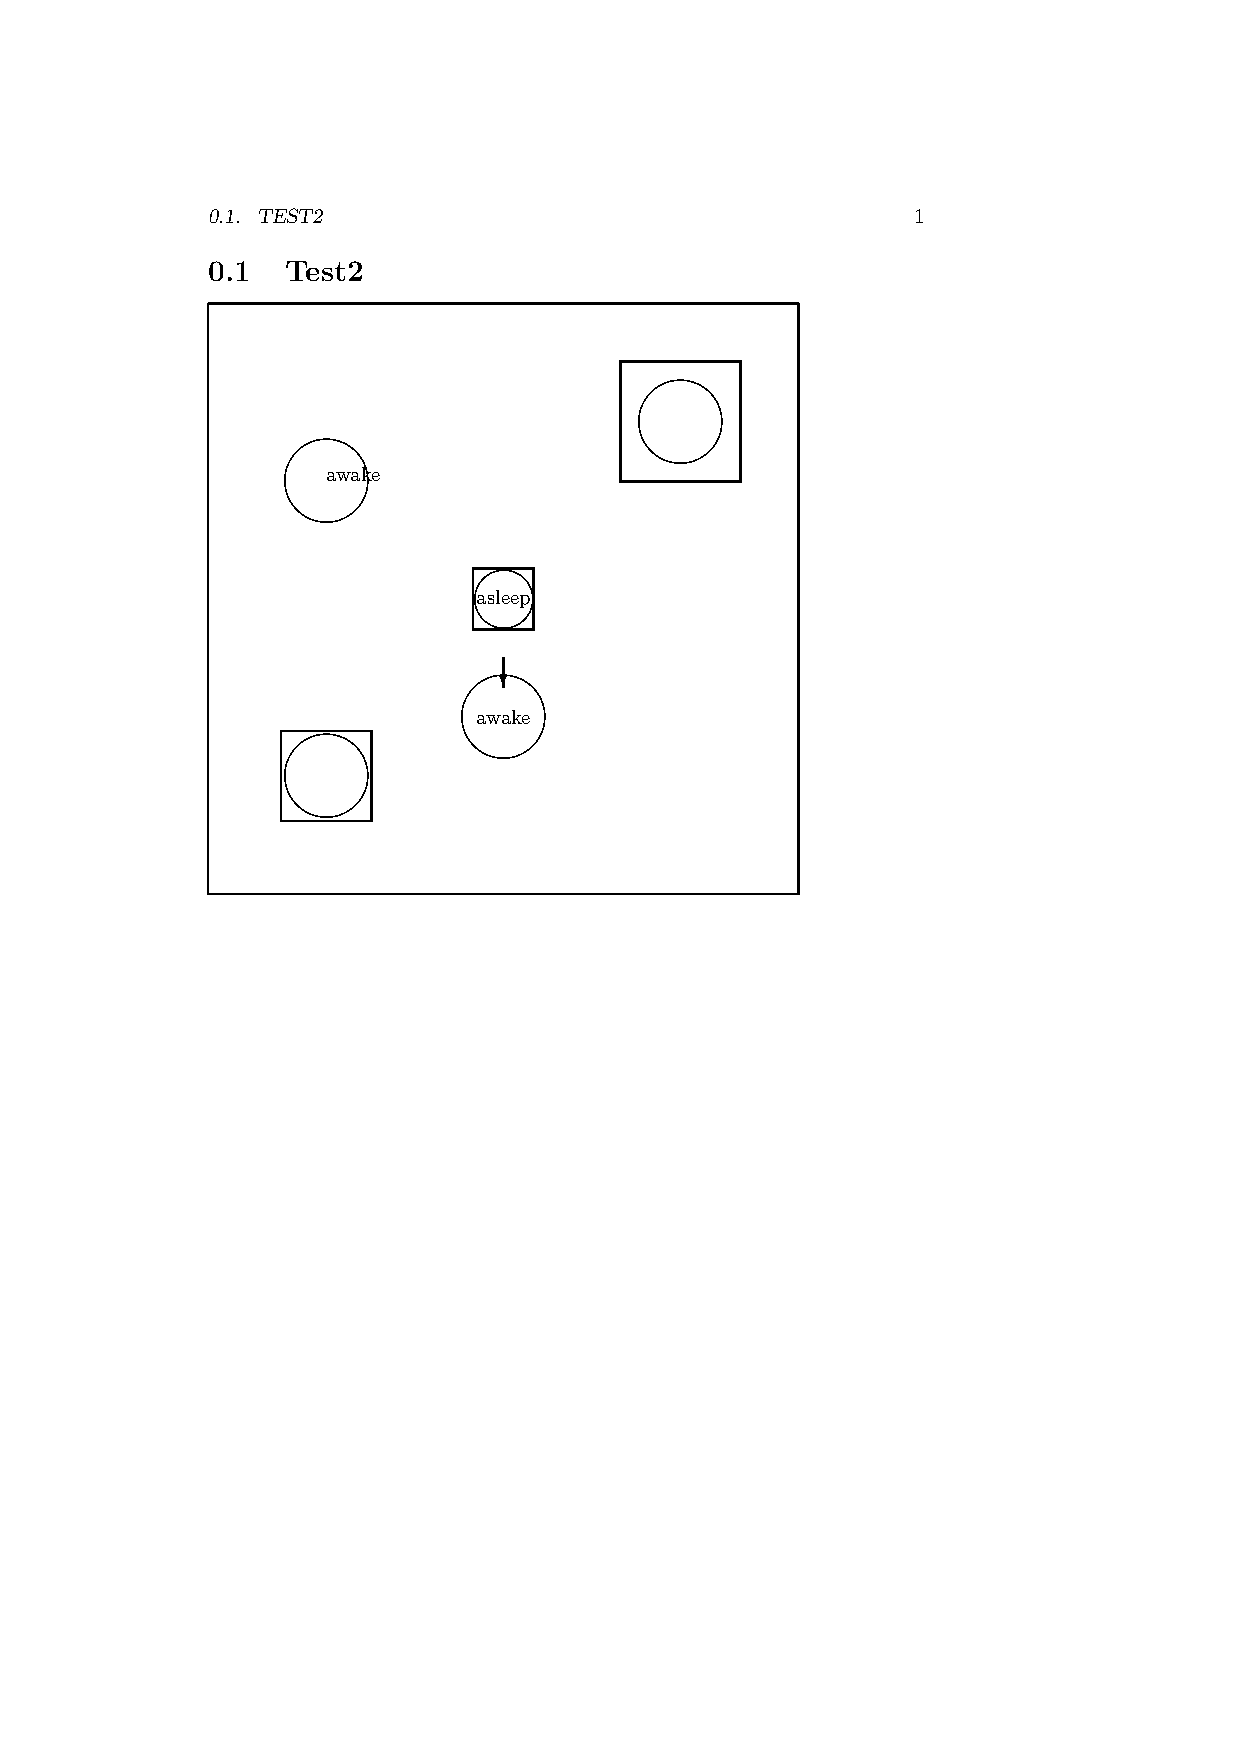
\includepdf[pages=-]{anhang/beispielanhang}	% pages=- bedeutet: alle Seiten | Wie bei Bilder die Dateierweiterung (.pdf) am besten weglassen
% % Weites Beispiel: Nur Seiten 1-2 und 4, Papier querformat mit 2 Seiten pro Seite
% %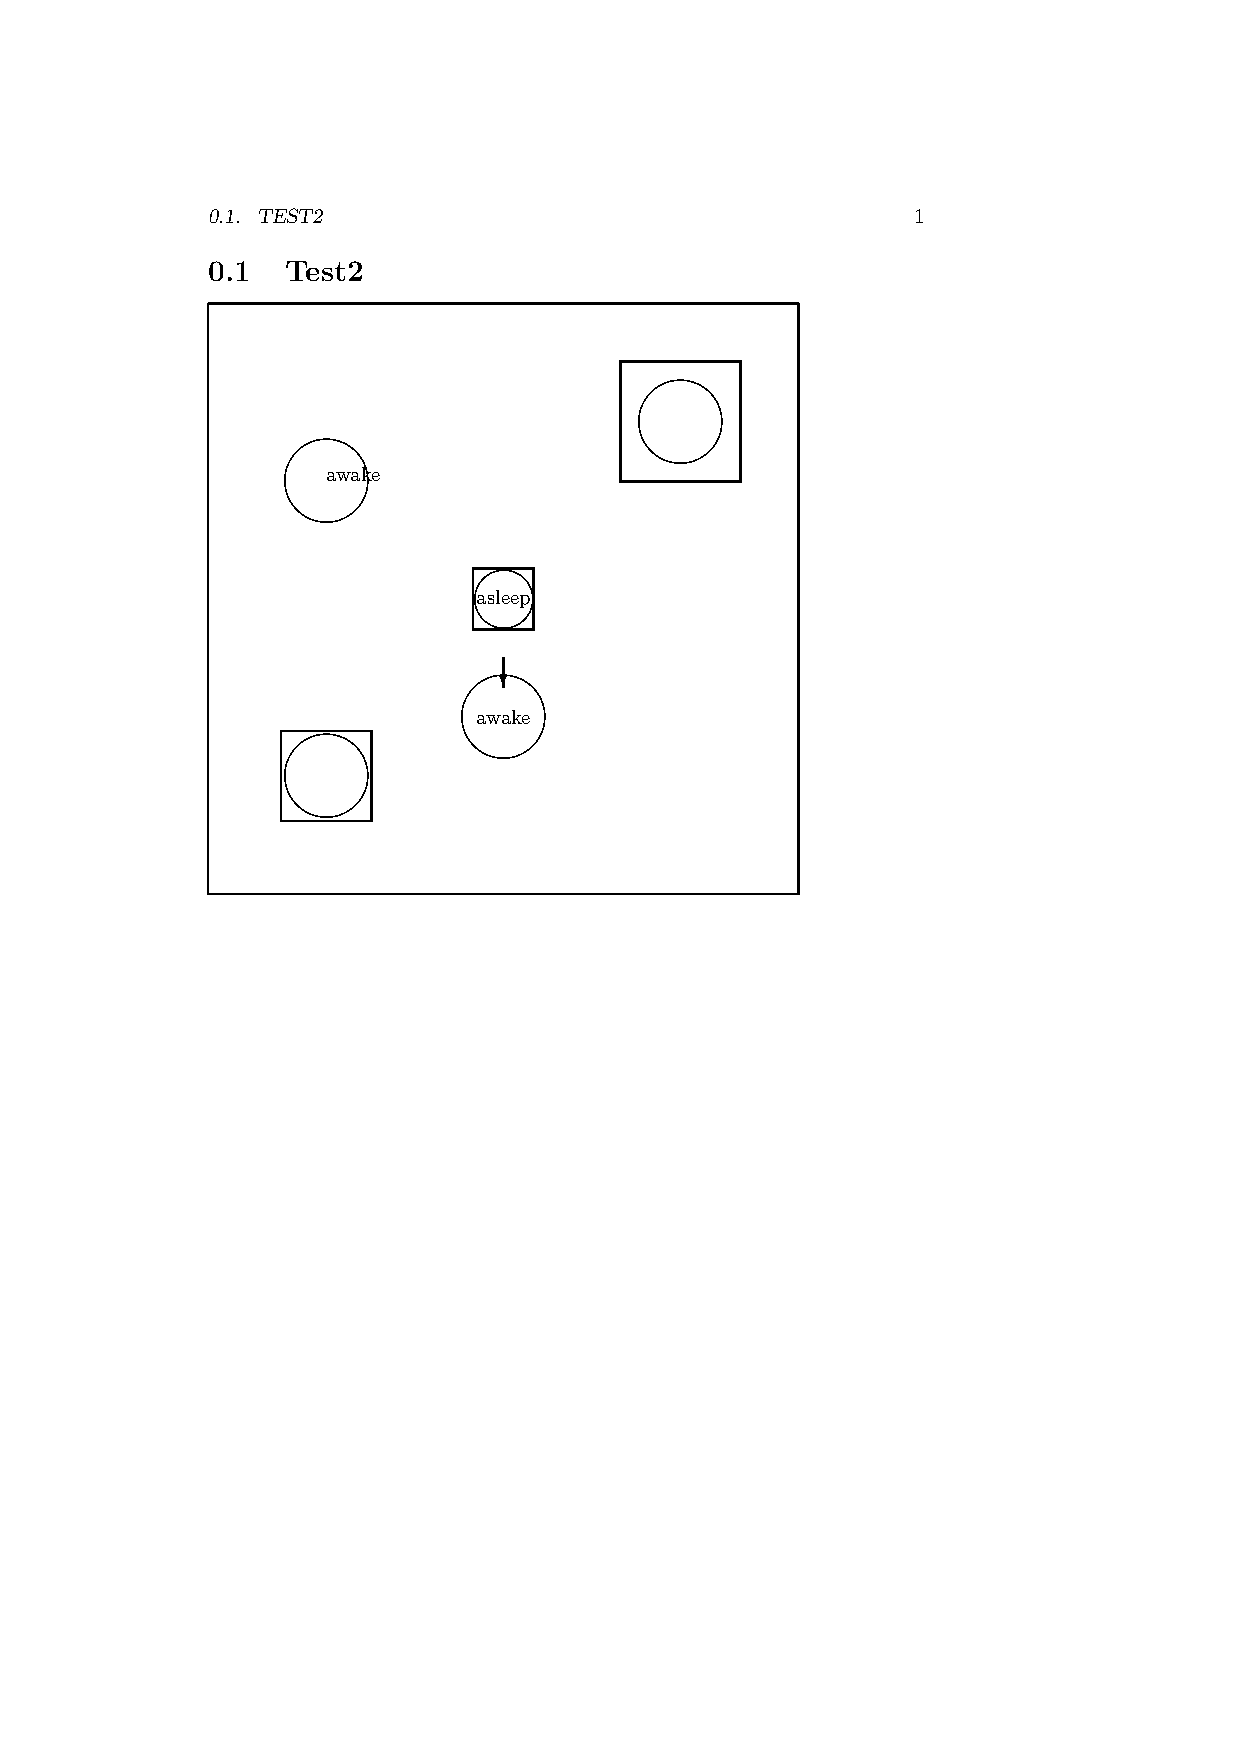
\includepdf[pages={1-2,4},landscape,nup=1x2]{anhang/beispielanhang}
% 
% \else  % bei der Verwendung vom normalen LaTeX:
% \newpage
% \addtocounter{page}{5}	% Seitenz�hler hochz�hlen und Anhang nach dem Drucken manuell hinzuf�gen
% % Hier wurde angenommen, dass der Anhang f�nf Seiten lang ist
% \fi
% 
% \chapter{Weiterer Anhang}

%Erkl�rung, dass man alles selbst verfasst hat und alle Quellen offen gelegt
% wurden
%von diplomarbeit vorlage herauskopiert. anscheinend so standard in
% gummersbach\ldots

\newpage
%\chapter{Ehrenw�rtliche Erkl�rung}
%\thispagestyle{empty}

\Huge Erhenw�rtliche Erkl�rung\\\\

\normalsize

Ich versichere, die von mir vorgelegte Arbeit selbst�ndig verfasst zu haben. Alle
Stellen, die w�rtlich oder sinngem�� aus ver�ffentlichten oder nicht ver�ffentlichten
Arbeiten anderer entnommen sind, habe ich als entnommen kenntlich gemacht.
S�mtliche Quellen und Hilfsmittel, die ich f�r die Arbeit benutzt habe, sind
angegeben. Die Arbeit hat mit gleichem Inhalt bzw. in wesentlichen Teilen noch
keiner anderen Pr�fungsbeh�rde vorgelegen.

\vspace{9cm}
Gummersbach, den \today\\\\

\_ \_ \_ \_ \_ \_ \_ \_ \_ \_ \_ \\
Georg Wolf

\end{appendix}
%Leere Seite am Ende
\newpage\thispagestyle{empty}~

\end{document}

